%%% Local Variables:
%%% mode: latex
%%% TeX-master: t
%%% End:

\documentclass[bachelor]{thuthesis}
% \documentclass[%
%   bachelor|master|doctor, % mandatory option
%   xetex|pdftex|dvips|dvipdfm, % optional
%   secret,
%   openany|openright,
%   arialtoc,arialtitle]{thuthesis}

% 所有其它可能用到的包都统一放到这里了,可以根据自己的实际添加或者删除。
\usepackage{thutils}
\usepackage{hyperref}

% 你可以在这里修改配置文件中的定义,导言区可以使用中文。
\def\myname{卿培}

\begin{document}

% 定义所有的eps文件在 figures 子目录下
\graphicspath{{figures/}}


%%% 封面部分
\frontmatter

%%% Local Variables:
%%% mode: latex
%%% TeX-master: t
%%% End:
%\secretlevel{绝密} \secretyear{2100}

\ctitle{多视点视频的并行实时解码}
% 根据自己的情况选,不用这样复杂
\makeatletter
\ifthu@bachelor\relax\else
  \ifthu@doctor
    \cdegree{工学博士}
  \else
    \ifthu@master
      \cdegree{工学硕士}
    \fi
  \fi
\fi
\makeatother

\cdepartment[计算机]{计算机科学与技术系}
\cmajor{计算机科学与技术}
\cauthor{卿培} 
\csupervisor{孙立峰\ 副教授}
% 如果没有副指导老师或者联合指导老师,把下面两行相应的删除即可。
%\cassosupervisor{陈文光教授}
%\ccosupervisor{某某某教授}
% 日期自动生成,如果你要自己写就改这个cdate
%\cdate{\CJKdigits{\the\year}年\CJKnumber{\the\month}月}
\cdate{2010年6月22日}

%\etitle{Parallel real-time decoding of Multi-view codec(MVC) 3D video} 
% \edegree{Doctor of Science} 
%\edegree{Doctor of Engineering} 
%\emajor{Computer Science and Technology} 
%\eauthor{Qing Pei	} 
%\esupervisor{Associate Professor Sun Lifeng} 
%\eassosupervisor{Chen Wenguang} 
% 这个日期也会自动生成,你要改么?
% \edate{December, 2005}

\cleardoublepage
% 定义中英文摘要和关键字
\begin{cabstract}

视频编解码的并行在近几年CPU向多核方向发展之后成为一个热门的研究领域。最近成为标准的多视点视频由于其数据量庞大、编解码运算复杂,很难依靠单核的处理器达到实用的解码速度。因此,多核并行解码多视点视频势在必行。

我们以现有的多视点视频解码器为基础,通过对解码器函数级的优化,包括函数逻辑、减少循环内部的计算量、使用汇编实现部分函数,以及一个可以稳定运行的并行解码框架的实现,最终使得多视点视频的解码可以在主流PC上实现两路标清的实时解码。

本文的主要贡献是:
\begin{itemize}
\item 首次实现了非商业化的解码器在PC上的两路多视点视频实时解码;
\item 使用庞一等在2009年提出的多视点视频编解码并行调度框架\cite{pang2009framework}在解码器中实现了稳定的调度器。
\end{itemize}

\end{cabstract}

\ckeywords{多视点, 并行, 实时, 解码}

\begin{eabstract} 

With the multi-core trend of processor design and production, research efforts on the parallelization of video coding have been strengthened. Multi-view coding (MVC), which has been standardized recently, demands massive space for storage and an enormous amount of computation to encode and decode and therefore is therefore almost impossible to be decoded in realtime with a single processor core. A parallel decoder for multi-view coding is highly in demand.

On the basis of an available decoder, we apply multiple ways of optimization on function level, including rewriting the logic structure, decreasing the amount of computations inside loops and replacing some of the function body with assembler code. Meanwhile, a stable parallel framework for scheduling and decoding is implemented. All the optimizations add up to reach the performance guideline of realtime decoding of dual-view standard definition (SD) video on mainstream PC platforms.

The main contributions of this paper are
\begin{itemize}
\item to realize the first noncommercial decoder capable of decoding dual-view MVC video in real-time;
\item to implement a stable version of scheduler and decoder with the framework\cite{pang2009framework} put forward by Pang, et.al, in 2009.
\end{itemize}

\end{eabstract}

\ekeywords{Multi-view Coding(MVC), Parallel, Realtime, Decoding}

\makecover

{\shuji[多视点(\hspace{0.2em}\raisebox{2pt}{Multi-view Coding}\hspace{-0.25em} )视频的并行实时解码]}

% 目录
\tableofcontents

% 符号对照表
\begin{denotation}

%\item[HPC] 高性能计算 (High Performance Computing)
%\item[cluster] 集群
%\item[Itanium] 安腾
%\item[SMP] 对称多处理
%\item[API] 应用程序编程接口
%\item[PI]	聚酰亚胺
%\item[MPI]	聚酰亚胺模型化合物,N-苯基邻苯酰亚胺
%\item[PBI]	聚苯并咪唑
%\item[MPBI]	聚苯并咪唑模型化合物,N-苯基苯并咪唑
%\item[PY]	聚吡咙
%\item[PMDA-BDA]	均苯四酸二酐与联苯四胺合成的聚吡咙薄膜
%\item[$\Delta G$]  	活化自由能~(Activation Free Energy)
%\item [$\chi$] 传输系数~(Transmission Coefficient)
%\item[$E$] 能量
%\item[$m$] 质量
%\item[$c$] 光速
%\item[$P$] 概率
%\item[$T$] 时间
%\item[$v$] 速度
%\item[劝  学] 君子曰:学不可以已。青,取之于蓝,而青于蓝;冰,水为之,而寒于水。
%  木直中绳。(车柔)以为轮,其曲中规。虽有槁暴,不复挺者,(车柔)使之然也。故木
%  受绳则直, 金就砺则利,君子博学而日参省乎己,则知明而行无过矣。吾尝终日而思
%  矣,  不如须臾之所学也;吾尝(足齐)而望矣,不如登高之博见也。登高而招,臂非加
%  长也,  而见者远;  顺风而呼,  声非加疾也,而闻者彰。假舆马者,非利足也,而致
%  千里;假舟楫者,非能水也,而绝江河,  君子生非异也,善假于物也。积土成山,风雨
%  兴焉;积水成渊,蛟龙生焉;积善成德,而神明自得,圣心备焉。故不积跬步,无以至千
%  里;不积小流,无以成江海。骐骥一跃,不能十步;驽马十驾,功在不舍。锲而舍之,朽
%  木不折;  锲而不舍,金石可镂。蚓无爪牙之利,筋骨之强,上食埃土,下饮黄泉,用心
%  一也。蟹六跪而二螯,非蛇鳝之穴无可寄托者,用心躁也。\pozhehao{} 荀况
\item[CABAC] 基于上下文的自适应二进制算数编码(context-based adaptive binary arithmetic coding):CABAC的设计概念对于发生机率 > 0.5 的事件有效地编码,改进了传统霍夫曼编码法需要大量的乘法运算的问题,而在效能与压缩效率上取得相当大的改善空间。。
\item[CAVLC] 基于上下文的自适应变长编码(context-based adaptive variable-length code):适用于DCT转换后的整系数矩阵,经过zig-zag顺序扫描之后,在最高层的系数通常为+1/-1;又取得以zig-zag顺序扫描时,连续出现的0,或非零系数的总数、最后一个非零系数前零的数目等参数,作为查表时的坐标。CAVLC针对不同的块大小设计了不同的查找表,对各种不同的上下文, 使用不同的查找表进行编码,有效缩短输出比特流长度。。

\item[GOP]	group of pictures:一个GOP中所有帧的参有固定的参考结构;下一个GOP中的帧与上一个GOP中的帧的参考结构一样。

\item[MB]	宏块 (macroblock):一个16$\times$16的亮度块采样和对应的两个色度块采样。

\item[MVC]	多视点视频编解码 (multi-view video coding)。

\item[NAL unit] 网络抽象层(network abstract layer)单元:一个语法结构,包含后续数据的类型指示和所包含的字节数,数据以RBSP形式出现,必要时其中还散布有防伪字节。

\item[RBSB] 原始字节序列载荷(raw byte sequence payload):一个语法结构,包含整数个封装于NAL单元中的字节。RBSP或为空,或包含具有数字比特串形式的语法元素,其后跟随RBSP截止位和零个或多个连续的0值比特。RBSP的截止位为值为1的比特,RBSP的数据比特串的结束位置可以通过搜索RBSP中最后一个非零比特(截止位)得到。

\item[SODB] 数据比特串(string of data bits):表示语法元素的若干比特位的序列,出现在RBSP截止位之前。在SODB中,最左边的比特位是第一位并且是最高位,最右边的则是最后一位且是最低位。

\item[语法元素] syntax element:比特流中表示数据的元素。

\item[语法结构] syntax structure:零个或多个语法元素按照规定顺序一起出现在比特流中。

\end{denotation}



%%% 正文部分
\mainmatter

%%% Local Variables:
%%% mode: latex
%%% TeX-master: t
%%% End:

\chapter{引言}
\label{cha:intro}


\section{选题背景}
\label{sec:background}

21世纪的最初十年是计算机技术与互联网应用发展极为迅速的时期。在此期间,人们见证了CPU主频步入GHz时代,内存的容量和吞吐率按部就班地翻番,硬盘容量进入了TB级,人们探索互联网的接入方式也从曾经的56kbps甚至更慢的modem换成了带宽以Mbps计的宽带接入。可以说,这些都为数字多媒体技术在计算机和互联网上的应用奠定了硬件基础。

我们从十年前看VCD,五年前看DVD,到现在拥有了720p到1080p的高清电影资源;从8bit的音频到24bit、192kHz采样的无损音乐格式,无不需要计算能力更强和存储容量更大的计算机来处理。信息化的大步跨越让多媒体技术在我们日常生活中扮演越来越重要的角色。各种新的应用也接踵而来。

%3D电视的发展
3D电视经过多年的发展,已经逐渐走向成熟。在CES(Consumer Electronics Show) 2010的展厅里,“3D”成了最大的赢家,备受关注。Panasonic的VT25平板3D电视也获得了这届CES的“Best in Show Award”。无论是各大家电厂商展台上的3D电视,还是可以用在现有系统上的nVidia 3D Vision套装,都令消费者们感受到了3D时代即将来临。其实,3D电视的起源并不比2D电视晚很长时间\cite{smolic2007coding},但是由于其对计算、存储和传输的资源消耗比普通2D电视高出一倍甚至数倍,所以一直以来未能普及。

%3D视频编码的发展
为了满足资源有限条件下的3D视频应用,各种编码技术陆续诞生,以一定量的比特率来描述多视频信号,达到一定的压缩率,同时尽可能减小失真。在这个过程中,国际标准化组织应运而生。目前国际上有两个音视频编码标准化组织:
\begin{itemize}
\item 一是国际电信联盟标准化组(ITU-T)下属的视频编码专家组(VCEG:Video Coding Expert Group)。制定了一系列视频通信协议和标准,包括H.261、H.263、H.263+、H.264等。主要应用在视频通信领域,如视频会议等。
\item 二是国际标准化组织(ISO)和国际电工委员会(IEC)下属的运动图像编码专家组(MEPG:Motion Picture Expert Group)。自1988年成立以来,研究和开发了多种多媒体压缩标准,包括MPEG-1、MPEG-2、MPEG-4、MPEG-7等。主要应用在存储媒介(DVD)、广播电视网、有流媒体传输等。
\end{itemize}
\begin{figure}[htbp]
\begin{center}
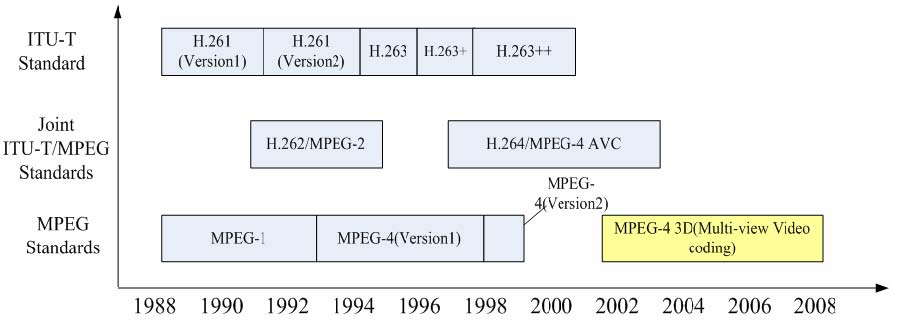
\includegraphics[width=\textwidth]{codecroadmap.png}
\caption{MPEG、VCEG、JVT视频编解码标准的发展}
\label{fig:codecroadmap}
\end{center}
\end{figure}

在2001年6月,经过评估发现,H.26L编码技术基本能够满足MPEG的标准需求,因此MPEG与VCEG的成员共同成立了一个新的工作组JVT(Joint Video Team),来推动和管理H.26L的最后标准化开发,并在2003年形成了视频标准,同时被MPEG和VCEG采纳:MPEG将其定为MEEG-4 part 10,VCEG将其定为H.264。MPEG和VCEG制定的主要标准见。H.264/MPEG-4 part 10标准称为高级视频编码(AVC:Advanced Video Coding),扩展性较好,用于3D视频的多视点视频编解码(MVC:Multi-view Video Coding)就是其一个扩展。MPEG与VCEG及JVT制定的主要视频标准如图\ref{fig:codecroadmap}所示。

\section{已有研究}
\label{sec:previouswork}

%MVC相关工作

在Multi-view Video Coding方向的研究在很久前就开始了。3D视频的一个特点是:传输给用户的各个视角的视频描述的是同一个场景。各个视角的视频在统计意义上的相关性很大,这些相关性就可以用来做预测,如图\ref{fig:mvcpredstruct}所示\footnote{http://mpeg.chiariglione.org/technologies/mpeg-4/mp04-mvc/image004.jpg}。综合利用时间序列以及视角间的图像预测结构,能够极大地提高编码效率\cite{merkle2005statistical}\cite{kaup2006analysis}。\onlinecite{magnor2003multi}中提及了多视点图像编码的一些前沿研究。
\begin{figure}[htbp]
\begin{center}
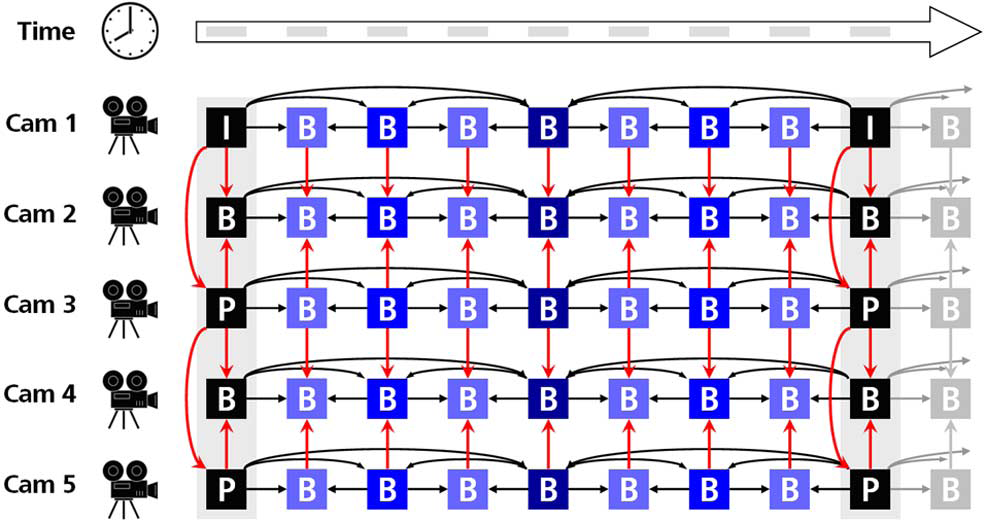
\includegraphics[width=\textwidth]{mvcpredstruct.png}
\caption{MVC的时间和视角间预测结构}
\label{fig:mvcpredstruct}
\end{center}
\end{figure}

对于视角间和时间序列上的图像预测结构,有不少文献提出了不同的方法。其中,H.264/AVC时间和视角间预测的基于B帧的算法\cite{kaup2006analysis}在MPEG标准测试下性能表现最好\cite{flierl2007motion}\cite{merkle2006efficient}\cite{mueller2006multi}\cite{merkle2007efficient}。在实验中,各种指标都显示MVC远远超越了独立压缩每个视角视频的方法。不过,能够获得的性能提升对参数有一定依赖,如相机间距、帧率、内容复杂度(运动和纹理)等属性。对于一些数据集,信噪比峰值(PSNR)的增益在0.5dB以下,而最大的增益能达到3dB。

这个方法在提高视频编码压缩率的同时,增加了编解码的复杂度,要求处理更大量的数据和进行更多的计算。对于MVC编解码的研究大多使用参考软件JMVC进行\footnote{由Heiko Schwarz、Tobias Hinz、Karsten Suehring等人开发。}。参考软件的编写比较注重对应多视点视频编码的原理,对于学习MVC编解码很有帮助,但也因此损失了极大的性能。在实验所使用的机器上对720$\times$576的两路视频进行编码,19帧需要大约半个小时,这远远不够实际应用的需求。诺基亚研究中心(Nokia Research Center)针对其运行Maemo的平台开发了一款MVC实时解码器\footnote{http://research.nokia.com/research/mobile3D},针对单核心做了不少优化。由于其主要利用汇编优化,而处理器并不是x86兼容的,所以不易移植到PC上。

至此,我们认为有必要进行一个能够在PC上进行两路到更多路MVC视频的解码器,进行客户端的实时解码。这样的解码器是3D视频应用普及的一个重要前提。

由于MVC是H.264/AVC的一个扩展,所以我们首先想到H.264的并行编解码问题。这个方向近几年有一些文献:\onlinecite{li2005design}提出的算法使用一个处理器进行动量估计以外的运算,其余处理器进行运动向量的估计。\onlinecite{seitner2007macroblock}做了H.264解码器的宏块并行分析,\onlinecite{mesa2009scalability}给出了H.264解码器宏块并行算法。而更进一步针对多视点视频的并行解码的研究相对较少:\onlinecite{yang2006parallel}提出了一种超空间(hyper-space)的方法,\onlinecite{ugur2007parallel}通过对参考帧施加一定限制条件使得解码器等待参考帧传入的时间大幅降低,从而提升并行解码速度。

%庞一等 论文
庞一等在2009年提出了一种多核架构上并行处理多视点视频的启发式调度框架\cite{pang2009framework}。不同于以往的帧并行或宏块并行的研究,提出了通过优化解码任务调度来提高解码器并行性能的观点,并通过实验证明性能的大幅提升。该方法对多视点视频的调度如图\ref{fig:gopschedulinginmvc}所示,通过重新安排帧解码顺序,最小化多路视频解码时因为等待参考帧传入和其解码结果的等待时间,从而加快解码速度。
\begin{figure}[htbp]
\begin{center}
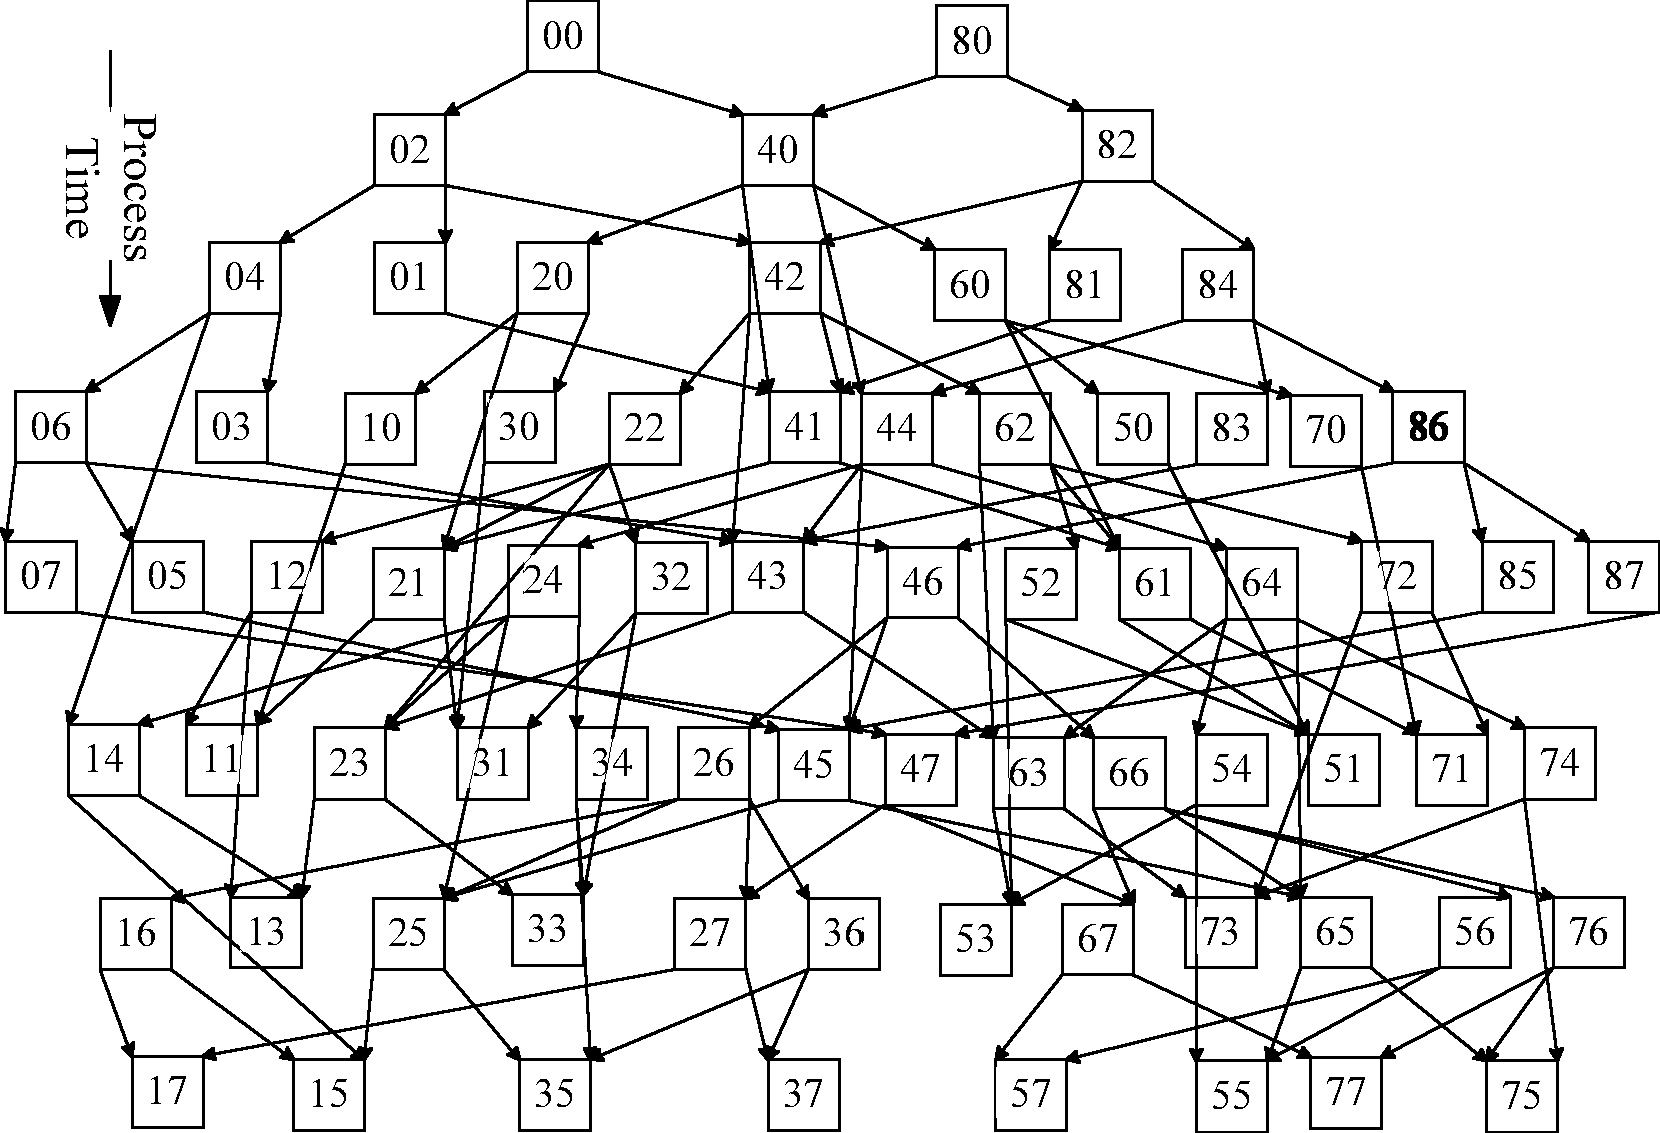
\includegraphics[width=\textwidth]{gopschedulinginmvc.png}
\caption{多视点视频种的GOP调度}
\label{fig:gopschedulinginmvc}
\end{center}
\end{figure}


%MVC Decoder工作
在此基础上,我们已经实现了一个成型的多视点视频编解码系统,包括编码器和解码器。编码器将若干YUV格式的视频编码为一个MVC视频。解码器将一个MVC视频解码为N个独立的YUV视频,N为该MVC视频包含的视角数量。编解码结果符合MVC的标准\cite{iso2009mvc}。

在第\ref{cha:decoderprincipleandrealization}章中将进一步介绍解码器部分。

\section{本文的任务}
\label{sec:workbrief}

目前已有的MVC Decoder工程速度较慢,不能满足实时解码播放的要求。本文主要通过针对单核和多核结构的优化,是现有的MVC解码器能够在CPU上做到至少两路分辨率为720$\times$576的视频的实时解码。

此外,由于MVC视频的标准尚未确定,硬件也尚未普及,还没有一种播放器能够支持各种硬件平台上的MVC视频播放。我们的实验环境有Bolod的3D平板电视和nVidia的3D Vision眼镜套装,为了实现一个从采集到播放的完整系统,除了解码器的优化以外,我还需要设计实现一个3D播放器,让用户能够看到三维的播放效果。

\section{本文的结构}
\label{sec:thesisstructure}

本文第\ref{cha:decoderprincipleandrealization}章介绍需要优化的多视点视频解码器的原理和实现。第\ref{cha:optapproach}章说明我进行解码器性能优化的基本思路。第\ref{cha:singlecoreopt}章和第\ref{cha:parallelopt}章分别详述单核心性能优化和多核处理的并行优化过程。第\ref{cha:optresultandanalysis}章介绍实验结果并进行了一定的分析。第\ref{cha:conclusionandforesight}章总结优化工作并对下一步的工作有所展望。

同时进行的3D播放器设计与实现部分与解码器优化不相关,所以不列在章节中,单独作为附录\ref{cha:3Dplayerdesignandrealization}附在正文之后。

%%% Local Variables: 
%%% mode: latex
%%% TeX-master: t
%%% End: 

\chapter{MVC解码器原理与实现}
\label{cha:decoderprincipleandrealization}

%参见胡伟栋论文和张凤研论文
自2006年起,胡伟栋等开始着手编写一套视频编解码系统。至2010年初基本完成,编解码的过程基本符合MVC标准\cite{iso2009mvc}的描述。编写过程中,主要参考了《H.264 and MPEG-4 video compression, video coding for next-generation multimedia》\cite{richardson2003h}、T264项目\footnote{\href{http://sourceforge.net/projects/t264/}{http://sourceforge.net/projects/t264/}}和JMVC参考软件。代码参考了JMVC的框架设置。

\section{参考软件JMVC介绍}
\label{sec:introtojmvc}
JVT在发布MVC草案的同时还发布了MVC编解码的参考软件JMVM(Joint Multi-view Video Model)。MVC标准确立之后,JMVM改名为JMVC(Joint Multi-view Video Coding),陆续有新版本发布。我们的编解码器起初参考的是JMVC 4.2版,今年由于新发布的JMVC 7.2编解码结果与旧版并不兼容,我们又针对新版做了更正。

JMVC包括以下几个工程:
\begin{itemize}
\item H264AVCCommonLibStatic
\item H264AVCDecoderLibStatic
\item H264AVCEncoderLibStatic
\item H264AVCVideoIoLibStatic
\item MVCBitStreamAssembler
\item MVCBitStreamExtractor
\item DownConvertStatic
\item PSNRStatic
\item H264AVCDecoderLibTestStatic
\item H264AVCEncoderLibTestStatic
\end{itemize}

其中,DownConvertStatic是为了前向兼容;PSNRStatic是进行编码质量分析,与MVC编解码实现无关,不做介绍。

H264AVCCommonLibStatic包含编解码时都需要的一些函数,例如对读取一帧的属性、各类Filter函数、量化与反量化函数、宏块的变换与反变换操作等等。H264AVCDecoderLibStatic就是解码器的函数库,H264AVCEncoderLibStatic则是编码器函数库。H264AVCVideoIoLibStatic是进行视频文件读写操作的函数库。

由于MVC视频文件可能包含多路H.264视频,所以需要对码流进行打包,MVCBitStreamAssembler就是这个模块;相应的,MVCBitStreamExtractor就是从码流中抽取各路视频的模块。

除了函数库之外,JMVC还提供了两个工程演示调用库函数进行MVC编码和解码的过程,分别在H264AVCEncoderLibTestStatic和H264AVCDecoderLibTestStatic中。

\begin{figure}[htbp]
\begin{center}
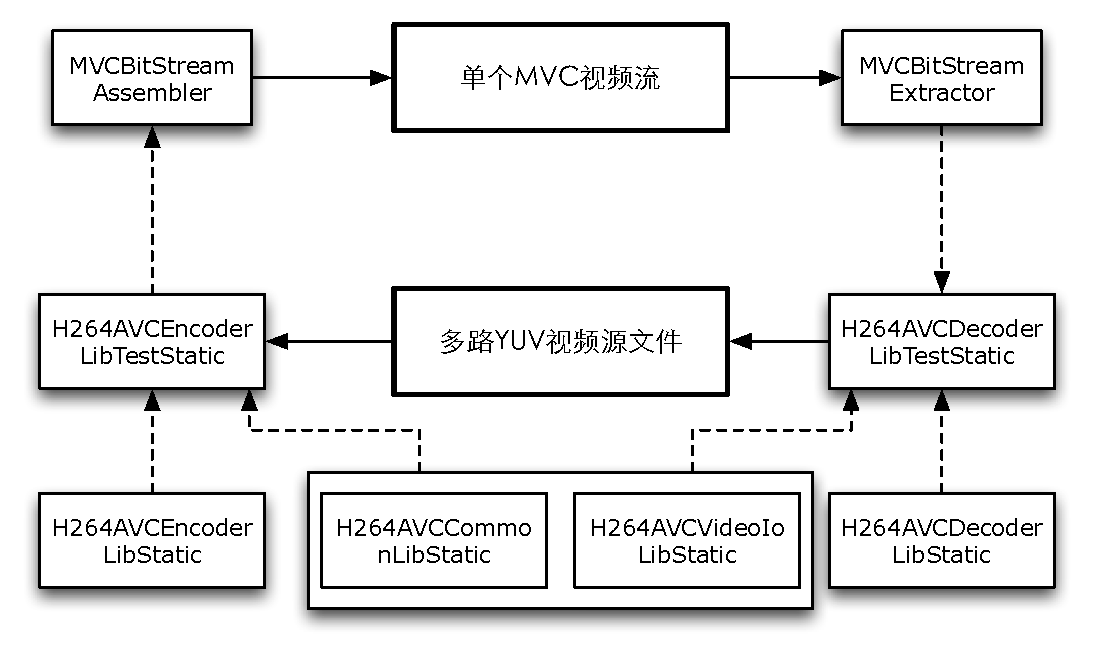
\includegraphics[width=\textwidth]{JMVCstructure}
\caption{JMVC编解码框架}
\label{fig:JMVCstructure}
\end{center}
\end{figure}

利用JMVC进行编解码的框架如图\ref{fig:JMVCstructure}所示。

编码器的输入为若干路YUV视频,一般是同一场景从若干不同角度拍摄的视频,有相同的分辨率并且经过时间同步和校准。YUV文件要求是4:2:0格式,每$2\times2=4$个像素由一个$2\times2$的亮度矩阵和两个$1\times1$的色度矩阵。亮度矩阵顾名思义表示了4个像素的亮度,两个色度矩阵表示像素红蓝两色的平均色度,如图\ref{fig:Barn-yuv}所示。
在编解码器开发期间,庞一、胡伟栋、张凤研等对编解码在帧级别的并行性进行了深入研究\cite{pang2009adaptive,yi2008parallelized},并在编码器和解码器中都采用了帧并行的算法。

\begin{figure}[htbp]
\begin{center}
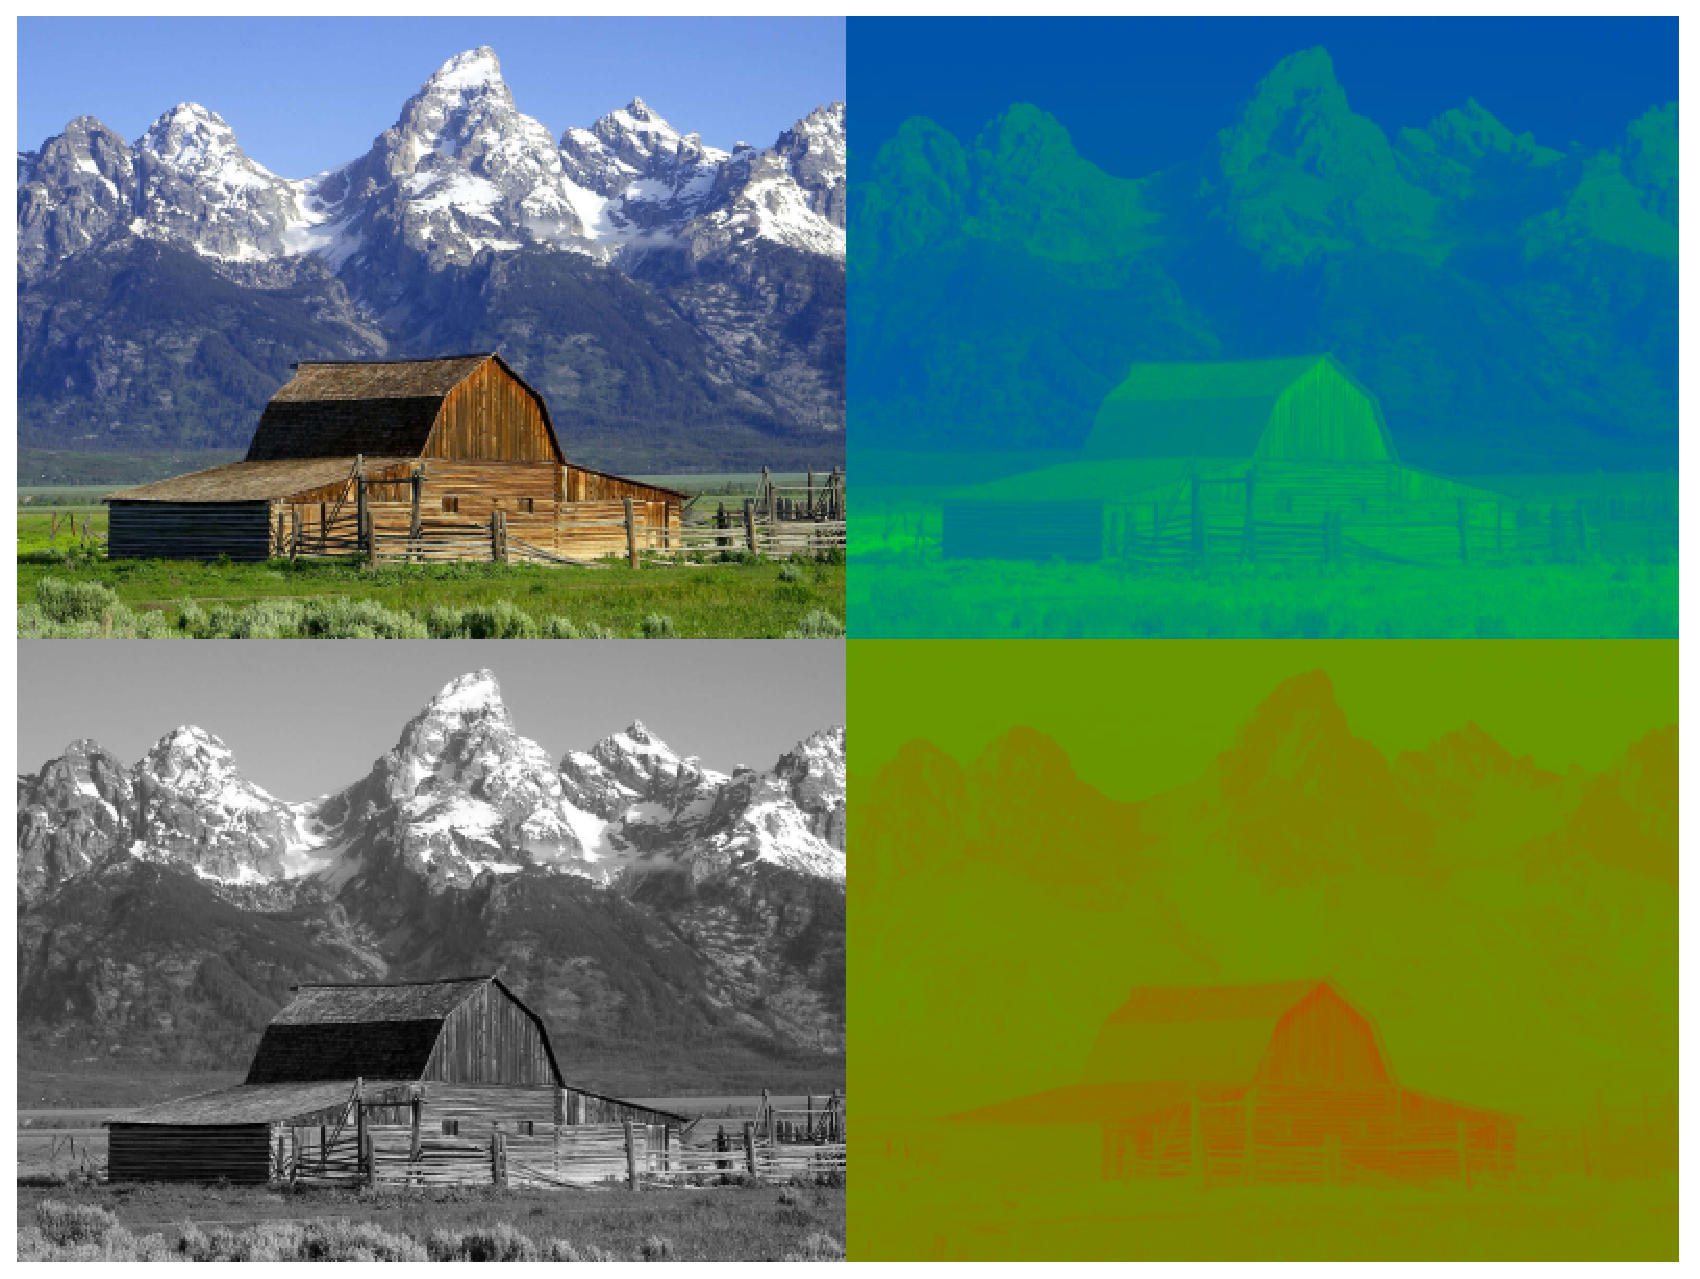
\includegraphics[scale=0.4]{Barn-yuv.eps}
\caption{原始图像(左上)和其Y'(左下)、U(右上)、V(右下)分量}
\label{fig:Barn-yuv}
\end{center}
\end{figure}

\section{自主开发的MVC解码器}
\label{sec:mvcdecoder}
%TODO 解码流程图
%TODO 解码器行为描述

%%% Local Variables: 
%%% mode: latex
%%% TeX-master: t
%%% End: 

\chapter{解码器性能优化方案}
\label{cha:optapproach}

毕设工作的主体是解码器性能优化,本章主要介绍性能优化的一些准备工作并提出优化方案。

\refsec{sec:platformdesc}介绍了实验所用的软硬件平台。\refsec{sec:decoderprofiling}介绍了对解码器进行性能分析的方法与结果,\refsec{sec:optapproach}以此为基础给出了性能优化的基本方案,最后在\refsec{sec:optaim}中说明了优化的目标。

\section{软硬件平台说明}
\label{sec:platformdesc}

我们的解码器支持多种硬件平台,包括x86、CELL等处理器;多种操作系统,包括Linux和Windows。本文所做的优化如无特殊说明,皆与软硬件平台无关,可以直接在其他平台上应用。为了方便实验,实验主要在以下环境下进行:

\begin{itemize}
\item {硬件平台}

\begin{itemize}
\item Intel Core2 Quad Q9400 @ 2.66GHz
	\footnote{禁止了SpeedStep功能}
\item 4GB DDR2/800 Memory
\item NVIDIA GeForce GTS 250 with 512MB
\end{itemize}

\item {软件平台}

\begin{itemize}
\item Microsoft Windows XP Professional SP3
	\footnote{Lenovo ThinkCenter M6100T预装操作系统}
\item NVIDIA WHQL Driver v197.13
\item DirectX 9.0c
\item Microsoft Visual Studio 2008 SP1
	\footnote{获取自:\href{http://helpdesk.tsinghua.edu.cn/yhfw/yhfw_zbrj_tz.jsp}{清华大学校园正版软件服务}}
\item CUDA SDK 3.0
\item Intel VTune Performance Analyzer 9.1 Build 385
	\footnote{30天评估版,序列号为VVVC-BDGCWFJC}
\item Intel C++ Compiler Professional 11.1.038
	\footnote{授权同VTune}
\end{itemize}

\end{itemize}


\section{解码器性能分析}
\label{sec:decoderprofiling}

对解码器进行优化的过程中,首先需要对其现有的性能表现有一个细致的了解。对于每一个函数的被调用次数、运行时间、运行时间百分比等指标都需要有较为精确的测量,才能更好地进行接下来的优化。

对此,我使用了两个性能分析工具来分析MVC Decoder工程。分别在接下来两节中说明。

\subsection{VS2008内置性能分析}
\label{subsec:vsprofiling}
Visual Studio 2008 Team System版内置了一个Analyze功能,可以对目标程序进行性能分析。性能分析有两种:
\begin{itemize}
\item 一种是不改变编译结果,通过运行时采样,得到每个采样时刻正在运行的函数,经过汇总后得到函数在采样上的分布情况,由此估计每个函数运行时间占总运行时间的百分比。这种方式称为Sampling方式。
\item 另一种是在编译时加入一些辅助代码,运行时通过这部分代码来标志进入和推出一个函数的时间,借助这些隐藏的输出信息得到总运行时间在各个函数内部的分布。这种方式称为Instrumental Code方式。
\end{itemize}

\subsubsection{性能分析步骤}
\label{subsubsec:profilingprocess}

在VS2008的菜单中有一个“Analyze”项,选择“New Performance Wizzard”打开一个性能分析向导。

选择要分析的项目、分析的方式之后就可以开始分析了。

成功执行植入了instrumental code的可执行程序之后,profiling工具收集到大量的数据。经过一段时间(在我的机器上大约两分钟)的处理,会给出一个性能分析报告。

\subsubsection{性能分析结果}
\label{subsubsec:reportexerpt}

性能分析报告中的FunctionList视图给出了各个函数(包括系统调用)占用的时间、时间的百分比以及被调用次数等等数据。我们关心的是其中的“Exclusive Time”、“Number of Calls”两列。当然,“Exclusive Time \%”也被我们选中,因为百分比相对于毫秒数能让我们更直观地了解函数占用的时间。

% Table generated by Excel2LaTeX from sheet 'MVCDecoder100611_FunctionSummar'
\begin{table}[htbp]
  \centering
  \begin{minipage}[t]{\linewidth}
  \caption{VS2008性能分析报告(前10项记录)}
  \label{tab:vs10}
	\rowcolors[]{1}{white}{gray!15}
    \begin{tabular}{lrrr}
    \addlinespace
    \toprule[1.5pt]
    \textbf{Function Name} & \textbf{Exclusive Time\footnote{不包括函数体内调用其他函数的净运行时间}} & \textbf{Exclusive Time} \% & \textbf{Number of Calls\footnote{函数被调用次数}} \\
    \midrule[1pt]
    macroblockPredGetDataUV & 341.01 & 14.41 & 2,632,478 \\
    macroblockPredGetDataY & 321.37 & 13.58 & 1,316,239 \\
    idct4x4\_c & 316.86 & 13.39 & 5,028,960 \\
    macroblockGetPred\_axb & 181.29 & 7.66  & 1,316,239 \\
    macroblockGetPred\_axb\_Bi & 133.42 & 5.64  & 571,944 \\
    macroblockGetHalfPel & 132.47 & 5.6   & 148,552 \\
    Filter & 101.92 & 4.31  & 6,215,308 \\
    addMacroblockdata & 85.36 & 3.61  & 184,171 \\
    iquant4x4\_c & 84.48 & 3.57  & 5,028,960 \\
    macroblockPBPrediction & 70.95 & 3     & 184,171 \\
    \bottomrule[1.5pt]
    \end{tabular}
  \end{minipage}
\end{table}


分析报告中仅仅MVCDecoder.exe自身的函数就有近200条记录,而大部分都占用不足$0.05\%$的时间,优化价值不大。在\autoref{tab:vs10}中我们给出了时间占用排在前10的记录。更详细的记录参见\autoref{cha:expdatatable}中的\autoref{tab:vs50}。

\subsection{VTune分析}
\label{subsec:vtuneprofiling}

在实验过程中,我们发现大部分函数运行总时间没有明显差别,与我们进行项目合作的北京世纪鼎点软件有限公司的罗翰先生指出,VS2008的性能分析可能不够准确,使用Intel的VTune或许能够得到更准确的性能分析结果。

关于Intel VTune如何精确地进行性能分析,文\onlinecite{levinthal2007,levinthal2006,levinthal2008,levinthal2008a}中有介绍。

\subsubsection{性能分析步骤}
\label{subsubsec:profilingprocess}

打开VTune Performance Analyzer之后,我们新建一个工程,选择采集call graph数据。配置好要运行的可执行文件和执行路径就可以开始分析了。与VS2008的分析一样,经过一段时间的执行和数据处理,我们获得一个性能分析报告。

\subsubsection{性能分析结果}
\label{subsubsec:reportexerpt}

% Table generated by Excel2LaTeX from sheet 'VTune_FunctionSummary'
\begin{table}[htbp]
  \centering
  \caption{VTune性能分析报告(前10项记录)}
  \label{tab:vtune10}
  	\rowcolors[]{1}{white}{gray!15}
    \begin{tabular}{lrrr}
    \addlinespace
    \toprule[1.5pt]
    \textbf{Function Name} & \textbf{Number of Calls} & \textbf{Exclusive Time (ms)} & \textbf{\% in Function} \\
    \midrule[1pt]
    macroblockPredGetDataUV & 2632478 & 774863 & 0.61 \\
    macroblockPredGetDataY & 1316239 & 702575 & 0.58 \\
    idct4x4\_c & 5028960 & 398076 & 1 \\
    macroblockInterDecode16x16\_y & 184171 & 328834 & 0.46 \\
    macroblockGetPred\_axb & 1316239 & 311730 & 0.11 \\
    FilterMB & 210600 & 203506 & 0.21 \\
    Filter & 6215308 & 191937 & 1 \\
    iquant4x4\_c & 5028960 & 157459 & 1 \\
    macroblockInterDecode\_uv & 184171 & 154697 & 0.48 \\
    macroblockPBPrediction & 184171 & 150609 & 0.05 \\
    \bottomrule[1.5pt]
    \end{tabular}
\end{table}


性能分析报告包含一个函数调用关系图以及函数运行时间表,我们关注的是后者。表中大部分列与VS2008的分析结果是公共的,比如函数名、总时间、净时间等等。我们采集了与此前同样意义的几列数据,包括“Function”,“Calls”,“Self Time”和“\% in function”。我们在\autoref{tab:vtune10}中给出前10条记录。更详细的记录参见\autoref{tab:vtune50}。


\subsection{性能分析结果说明}
\label{subsec:commentonreport}

我们观察两个分析结果\autoref{tab:vs10}和\autoref{tab:vtune10}可以发现:虽然两个性能分析工具在结果上存在一些差别,但函数运行时间的排序大体上是一致的,耗时多的函数都排在表格靠上的位置,表中列出的前10位的函数有7个在两个表中都出现了。我们认为,可以根据性能分析的结果来确定函数优化的大体方向,优化的主要对象就是表中排在前列的函数。

对这些函数进行进一步观察,我们可以将它们分类:
\begin{description}
\item[简单函数多次调用] 典型的例子是idct4x4\_c和iquant4x4\_c。这两个函数的调用次数都在5028960次,这仅仅是解码65帧两路视频所需要的次数。对于这类函数,哪怕是性能上的一点点提升,都会因为巨大的调用次数而对总解码时间产生较大的影响。
\item[复杂函数] 典型的例子是macroblockGetHalfPel,这个函数仅仅执行148552次,单次执行时间是idct4x4c的14倍,iquant4x4c的53倍。这样的函数需要有很大幅度的优化才会在总时间中有所体现。
\end{description}

同时,我咨询了对整个系统十分熟悉的胡伟栋,他指出:耗时排在前列的函数大多是根据JMVC参考软件的逻辑来编写的,其考虑了一些工程上扩展的需要而非性能优先,因此有一定的提升空间。

\section{优化方案}
\label{sec:optapproach}

在经过几次组会讨论之后,我们确定了如下的几个优化方案,分别对不同类型的函数进行重写逻辑、优化循环、汇编优化和CUDA优化。从重写逻辑开始,一步步优化解码器性能,直到符合优化目标(见\refsec{sec:optaim})为止。

\begin{description}
\item[重写函数逻辑] 解码器中有一些函数的逻辑判断有多处重复,降低了性能。如果能够理清楚函数逻辑,修改函数内部执行的顺序,就能够加快一些速度。\\这样的优化在\refsec{sec:singlecorelogicopt}中有例子及说明。
\item[循环的优化] 对帧和宏块的处理常常有两层for循环便利一个$width\times height$的像素矩阵,逐像素进行操作。对于这样的函数,首先考虑是否能够将多次循环内的操作合并到少量循环,再考虑循环结构对cache的友好程度。\\这样的优化在\refsec{sec:singlecoreloopopt}中有例子及说明。
\item[汇编优化] 在项目讨论中,罗翰先生提出ffmpeg等开源的视频项目中可能会有一些变换的汇编优化版本,如果能够应用汇编优化,那么这些函数的性能将会有大幅度的提升。就此,我们考虑对一些函数进行汇编优化。\\ \refsec{sec:singlecoreasmopt}中进一步说明了汇编优化。
\item[CUDA优化] 视频处理中很常见的就是并行性无处不在,解码器的调度器保证了帧解码具有一定的并行性,而对帧和宏块内部的处理往往还有可以并行的for循环逐像素操作,利用GPU的大量核心进行简单操作可以加快这类操作的速度。
\end{description}

\section{优化目标}
\label{sec:optaim}

我们进行MVC解码器优化的目标是为了能让普通用户使用PC作为终端能够收看3D视频。在显卡尚未内置MVC硬解码器的情况下,目前所有的解码任务都交给CPU来完成。我们将优化的目标设定在用户使用主流CPU能够进行两路标清视频\footnote{关于视频分辨率,有标清\href{http://en.wikipedia.org/wiki/Standard-definition_television}{SDTV}、增强型标清\href{http://en.wikipedia.org/wiki/Enhanced-definition_television}{EDTV}和高清\href{http://en.wikipedia.org/wiki/High-definition_television}{HDTV}等制式,我们所说的标清指的是国内广泛使用的\href{http://en.wikipedia.org/wiki/Enhanced-definition_television}{EDTV}中的\href{http://en.wikipedia.org/wiki/Phase_Alternating_Line}{PAL}制式视频,分辨率为$720\times576$。}的实时解码。

量化的指标就是,用CPU进行两路分辨率为$720\times576$的视频,每一路都能达到30帧/秒,总计60fps的解码速率。

达到上述目标之后,我们的解码器就能够用来在双目3D显示平台下开展实际应用了。如果想要使用我们同时拥有的Bolod生产的裸眼观看的3D电视,则需要输出8路信号。这在目前的CPU软解码算法上较难实现,目前有两种解决方案,一种是直接利用GPU加速解码过程,软解8路信号;另一种是CPU解码出2路信号,再用GPU通过2路立体信号合成出8路需要的信号。前一种方式已经在NVIDIA的蓝光播放器中应用了,不过其解决方案并不开源;后一种两路信号合成八路信号的项目,清华大学媒体所的李化常师兄正在进行中。在2010年3月已经实现了合成算法,将两帧画面合成出八帧大约耗时1秒,目前正在进行算法的优化工作。

\section{小结}
\label{sec:sum3}
本章主要介绍了用Visual Studio内置的profiler以及Intel VTune对解码器进行性能分析的过程,给出了分析结果,列举了耗时最长的10个函数并对这些结果进行了一定的说明。针对性能分析结果,提出了优化方案,并明确了性能优化要达到的目标。

\cleardoublepage

%%% Local Variables: 
%%% mode: latex
%%% TeX-master: t
%%% End: 

\cleardoublepage

\chapter{解码器单核性能优化}
\label{cha:singlecoreopt}

按照\refsec{sec:optapproach}中提到的优化方案,我们对解码器的单核性能进行了若干优化。本章中列举其中具代表意义的部分。

\refsec{sec:singlecorelogicopt}详细介绍了对函数逻辑的优化,\refsec{sec:singlecoreloopopt}介绍了对循环的优化并举例说明,\refsec{sec:singlecoreasmopt}介绍了汇编优化,\refsec{sec:singlecoreothers}提及了其它一些优化。

\section{函数逻辑优化}
\label{sec:singlecorelogicopt}

在MVCCommonLib模块中,PBPridict.cpp文件中包含了一些宏块预测相关的函数。此前的性能分析结果\autoref{tab:vs10}中显示,其中的macroblockGetHalfPel()函数耗时较多。这是一个使用Finite Impulse Response(FIR)计算一个Luma块的half-pel的函数。具体算法参考了《H.264 and MPEG-4 video compression, video coding for next-generation multimedia》\cite{richardson2003h}第173页起的描述。

函数内的一部分源代码如下:
\begin{lstlisting}[caption = {macroblockGetHalfPel()函数片段(优化前)}, label = lst:macroblockGetHalfPelorig]
`\dots`
for (int i = 0; i < hw; ++i){
	for (int j = 2; j < hh - 3; ++j){
		pif->vdata_half[0][i][j] = `\dots`; //some expression of vdata_half[][][]
		                              //                  and vdata[][]
	}
}
for (int i = 0; i < hw; ++i){
	for (int j = 2; j < hh - 3; ++j){
		tmp[i][j] = `\dots`; //some expression of vdata[][]
	}
}
`\dots`
\end{lstlisting}

检查两次循环中对变量的访问,第二次循环需要访问vdata数组,而第一次循环只修改vdata\_half数组,对vdata没有做任何改动,所以两个循环可以合并成一个。

最后形成的代码如下:

\begin{lstlisting}[caption = {macroblockGetHalfPel()函数片段(优化后)}, label = lst:macroblockGetHalfPelopt]
`\dots`
for (int i = 0; i < hw; ++i)
	for (int j = 2; j < hh - 3; ++j){
		pif->vdata_half[0][i][j] = `\dots`; //some expression of vdata_half[][][] and vdata[][]
		tmp[i][j] = `\dots`; //some expression of vdata[][]
	}
`\dots`
\end{lstlisting}

这个优化使程序运行时间\footnote{这里所说的程序运行时间是指用release版本的解码器解码一个长度为65帧,分辨率为$720\times576$,路数为2的Multi-view视频所耗费的时间。下同。}缩短了1016ms\footnote{原始的版本总运行时间为26344ms。}。

同样在MVCCommonLib模块中的PBPridict.cpp里,macroblockPredGetDataY()和macroblockPredGetDataUV()函数也是运行耗时很多的函数,事实上,不论是Visual Studio还是VTune的分析结果,这两个函数都是占用时间最多的(见\autoref{tab:vs10}和\autoref{tab:vtune10})。

这两个函数大部分的时间耗费在memset和memcpy上。对于这些系统api的调用,我们无法作修改,但是仔细观察其逻辑,我们发现函数的逻辑判断结构可以做一定优化。

源代码如下:

\begin{lstlisting}[caption = {macroblockPredGetDataY()函数片段(优化前)}, label = lst:macroblockPredGetDataYorig]
`\dots`
if (x<0) x = 0;
if (x >= pif->sizeh) x = pif->sizeh - 1;
`\dots`
if (le < 0) le = 0;
if (le > 0)
	memcpy(pif->vdata[i]+dl, linef + sl, le);`\label{line:memcpy}`
`\dots`
\end{lstlisting}

由于pif->sizeh的物理意义决定了它必然是非负的,当x=0的时候不可能出现x>=pif->sizeh的情况,所以每次调用macroblockPredGetDataY()的时候,如果x<0,都做了多余判断。

le是int类型,所以当le<0时,顺序执行语句不可能出现le>0的情况,也存在多余判断问题。事实上,第\ref{line:memcpy}行的memcpy语句只有在le>=1的情况下才会执行,而当le<1时,le都会被赋值为0。

经过优化后的代码如下:

\begin{lstlisting}[caption = {macroblockPredGetDataY()函数片段(优化后)}, label = lst:macroblockPredGetDataYopt]
`\dots`
if (x<0) x = 0;
else if (x >= pif->sizeh) x = pif->sizeh - 1;
`\dots`
if (le < 1) le = 0;
else
	memcpy(pif->vdata[i]+dl, linef + sl, le);
`\dots`
\end{lstlisting}

对macroblockPredGetDataUV()的优化同理。这两个函数优化后,程序运行时间再次减少了437ms。

在macroblockGetPred\_axb()中,原始的程序一共用了超过20个if语句来决定如何进行预测。根据我在《数字逻辑设计》以及《计算机组成原理》课程中的实验经验,这样的多重if语句用switch语句替换不但能使代码逻辑更加清晰,而且能提高性能。这相当于是把许多串联的2位的MUX改写成一个多位的MUX。

此处优化使程序运行时间缩短了47ms。

\section{循环优化}
\label{sec:singlecoreloopopt}

% macroblockGetPred_axb 1031ms
macroblockGetPred\_axb()函数耗时在\autoref{tab:vs10}和\autoref{tab:vtune10}中分别列在第4和第5位,也是耗时极多的函数。除了上一节提到的if语句改写成switch语句之外,我们还对其进行了循环内部的优化。
\begin{lstlisting}[caption = {macroblockGetPred\_axb()函数片段(优化前)}, label = lst: macroblockGetPred_axborig]
`\dots`
for (i = 0; i < sizex; ++i)
	for (j = 0; j < sizey; ++j)
		pred->y[i+off_in_x][j+off_in_y] = pif->vdata_half[halfid][i+borderT][j+borderL];`\label{line:index}`
`\dots`
\end{lstlisting}

% 循环变量的声明
首先是循环变量的声明,根据我们的经验,编译器会对循环变量的声明放在循环体内部的写法做优化,至少在linux平台下的gcc会这样做。再加上将循环变量的声明放在循环内部可以避免变量在作用域之外被使用,所以我们将所有的循环变量声明全部移到循环体内部。

其次,我们观察代码发现有多处如\autoref{lst: macroblockGetPred_axborig}所示的循环。


这些循环内的操作有一个特点:使用包含循环变量的表达式作为数组访问的下标。

以\autoref{lst: macroblockGetPred_axborig}中第\ref{line:index}行为例,在整个循环中,计算了$sizex\times sizey$次$i+off\_in\_x$和$i+borderT$。实际上可以在内层循环外就进行计算,这样就只用计算$sizex$次,极大地减少了加法操作,同时大幅减少了变量访问次数:本来要访问两个变量,放在寄存器中,再做加法;现在只用访问一个计算好的变量即可。

优化后的代码如下:
\begin{lstlisting}[caption = {macroblockGetPred\_axb()函数片段(优化后)}, label = lst: macroblockGetPred_axbopt]
`\dots`
for (int i = 0; i < sizex; ++i){
	int ioffinx = i+off_in_x;
	int iboarterT = i+borderT;
	for (int j = 0; j < sizey; ++j)
		pred->y[ioffinx][j+off_in_y] = pif->vdata_half[halfid][iboarterT][j+borderL];
}
`\dots`
\end{lstlisting}

经过上述优化,程序运行时间缩短了1031ms。

% 循环内外层对cache的优化

\section{汇编优化}
\label{sec:singlecoreasmopt}

%此处说idct8x8
我们查找了一些文献,发现可以用MMX和SSE等扩展指令集来加速一些矩阵变换函数,例如idct8x8。
Intel Application Note AP-922\cite{intel-ap922}说明了如何用MMX和SSE加速DCT变换。AP-945\cite{intel-ap945}说明了如何用SSE2加速IDCT变换。

实际操作中,我们采用了Laurent Aimar、Loren Merritt、Holger Lubitz和Min Chen编写的SSE2-optimized H.264 iDCT代码替换C++实现的iDCT代码。

由于我们测试用的样例视频对idct8x8的使用远不及idct4x4频繁,所以这部分优化在程序运行时间上并没有明显的体现。这是由于我们目前主要测试的是H.264的Base Profile,当我们的解码器将来支持High Profile的时候,就会大量调用8x8的变换了。

\section{其它优化}
\label{sec:singlecoreothers}

% 内容相关的判断顺序微调
除了以上优化之外,我们还进行了一些细微的优化。

在每一路H.264码流的解码过程中,我们经常需要判断一些标志位的值,根据这些标志位来选择做什么样的操作。这往往是通过一系列的if-else判断实现的。这就出现了很多的选择分支,进入每个分支的概率是不同的。我们通过解码大量不同的视频文件,记录这些分支的选择情况,对判断的顺序进行了微调。将大概率的事件优先判断,执行相应的操作,省去了一些在进入分支之前的无效判断。

这样的优化对所有的测试样例平均提高1\%的性能。

% 编译器ICC
我们还尝试了更换编译器,使用Intel C++ Compiler Professional(见\refsec{sec:platformdesc})来替换Visual Studio包含的编译器。

用ICC编译的代码比VS默认编译器编译出来的代码快5\%到6\%。

\section{小结}
\label{sec:sum4}
本章主要介绍了对解码器进行优化,包括逻辑重构、循环优化、汇编优化以及其它(例如编译器)的优化。这些优化主要提高了单核解码性能。尽管有了这些优化,解码器的单核性能仍然不能满足需求,所以还需要做并行化,这一部分在下一章中展开。




%%% Local Variables: 
%%% mode: latex
%%% TeX-master: t
%%% End: 

\chapter{解码器并行优化}
\label{cha:parallelopt}

\section{对解码器并行性的分析}
\label{sec:parallelpossibility}

\section{并行框架介绍}
\label{sec:parallelstructurebrief}

\section{问题与解决}
\label{sec:parallelbuganddebug}

%%% Local Variables: 
%%% mode: latex
%%% TeX-master: t
%%% End: 

\chapter{解码器性能优化实验结果}
\label{cha:optresultandanalysis}

本章主要介绍对解码器优化结果的测试方法及结果。首先说明了生成测试数据的过程,然后使用这些数据对优化前后的解码器进行测试,对比结果。

\section{测试数据的生成}
\label{sec:optresultsgeneration}

测试数据采用\refsec{sec:introtojmvc}中提到的参考软件JMVC和ffmpeg\footnote{\url{http://www.ffmpeg.org/}}配合生成。ffmpeg用来将多种格式(如AVI、MP4)的视频转换为YUV格式。JMVC中的H264AVCEncoderLibTestStatic用来对N路YUV视频压缩成H.264流,MVCBitStreamAssemblerStatic用来将多路H.264打包成一个MVC视频流。我们测试的视频分为3类:一路、两路和八路的多视点视频。他们的生成方法较为类似,我们以八路视频为例,说明生成的具体方法:
\begin{enumerate}
\item 首先要编写一个描述视频压缩参数的配置文件,我们实际使用的配置文件之一见\autoref{lst:mvccfg}。其中比较关键的项为
\begin{description}
\item[InputFile] 输入的文件名格式,golf1表示输入的各路视频为golf1\_0.yuv、golf1\_1.yuv、\dots、golf1\_7.yuv。
\item[OutputFile] 输出的文件名格式,与InputFile类似。输出的文件扩展名为.264。
\item[SourceWidth] 待编码视频的水平分辨率\footnote{由于YUV视频的内容只是视频每一帧的实际数据,不像我们常使用的一些被包装在容器中的视频格式,并没有存储视频的分辨率、帧率等参数。},如320。
\item[SourceHeight] 待编码视频的垂直分辨率,如240。
\item[FrameRate] 待编码视频的帧率,如30.0。
\item[FramesToBeEncoded] 从YUV文件的第一帧算起,一共需要编码的帧数,如623。
\item[GOPSize] 参考结构中的GOP大小的上限,如4。对这个参数的设置影响参考结构的复杂程度。
\item[NumViewsMinusOne] 编码视频的路数减1,如7。
\item[ViewOrder] 各路视频的编码顺序,如0-2-1-4-3-6-5-7。
\end{description}
其它还有一些对每一路视频的参考结构的限定,我们采用与JMVC的demo中相同的参考结构。
\item 有了上述的配置文件MVC.cfg\footnote{文件名可以取任意合法的文件名,对扩展名没有要求。}之后就可以使用如下的命令来编码了\\H264AVCEncoderLibTestStatic.exe -vf MVC.cfg 0\\这个命令使用MVC.cfg中定义的参数对View 0进行编码。想要编码全部8路视频需要严格按照MVC.cfg中ViewOrder定义的顺序进行编码。
\item 编码生成了8个H.264码流之后,我们需要将其打包成一个文件。MVCBitStreamAssemblerStatic就是这样的一个packer,它也需要一个配置文件,样例见\autoref{lst:assemblercfg}。其中定义了输入输出的文件名以及视频的路数。这里对输入文件的列举顺序没有要求,只要文件与视角对应即可。使用如下命令可以将码流打包:\\MVCBitStreamAssemblerStatic.exe -vf assembler.cfg
\item 由于JMVC的编码器性能极其低下\footnote{我们编码这个分辨率为$320\times 240$,一共623帧的golf623.mvc总共耗费了近四个小时。},我们推荐使用批处理来依次执行这些编码命令,免去每隔十几或几十分钟需要人工进行下一步编码命令的输入操作。一个批处理的样例见\autoref{lst:batchEncode}。
\end{enumerate}

我们能够在网上获取的用于研究的YUV格式多视点样例视频片段大多是QVGA的分辨率,这一方面由于在我们进行多视点视频解码器优化之前,已有的编解码器性能很差;另一方面是由于YUV格式对数据几乎没有压缩,需要大量的存储空间\footnote{我们测试用的$1280\times 720$的两路视频,仅仅两秒左右(65帧)就需要$85.7$MB$\times2$的空间。}。我们的测试目标针对的是分辨率至少为$720\times 576$的视频,这样的YUV源很难获得,需要自己生成。

值得庆幸的是,NVIDIA为了推广其3D产品,在网站上提供了几段高清的两路视频片段。我们使用ffmpeg将其中分辨率为$1440\times 1080$的一个WMV视频转换成两路独立的YUV文件。
\begin{enumerate}
\item 我们首先使用了MPEG Streamclip\footnote{\url{http://www.squared5.com/}}将这个$2880\times 1080$的WMV裁剪成左右两个$1440\times 1080$的部分。分别存为left\_1440x1080.mp4和right\_1440x1080.mp4。
\item 使用如下命令将视频转为目标分辨率(如$1280\times 720$)的YUV视频:\\
ffmpeg.exe -y -i left\_1440x1080.mp4 -ss 41 -vframes 65 -s 1280x720 dualtest\_1280x720\_65f\_0.yuv\\
ffmpeg.exe -y -i right\_1440x1080.mp4 -ss 41 -vframes 65 -s 1280x720 dualtest\_1280x720\_65f\_1.yuv\\
这里我们转换了从第41帧起的65帧画面。
\item 对这两个生成的YUV视频用前文提到的JMVC编码的方法就可以编码并打包成两路的MVC测试视频了。
\end{enumerate}

我们还使用了一段电影$\mathit{Avatar}$的花絮$\mathit{The\ World\ of\ Pandora}$中的片段生成一路的测试视频。

使用如下命令生成YUV文件:

ffmpeg.exe -y -i The\_World\_of\_Pandora.mov -ss 15 -vframes 65 -s 1280x720 singletest\_1280x720\_65f\_0.yuv

再用JMVC编码打包成一路MVC视频。

至此我们生成了全部用于测试的MVC视频,进行测试用到的所有视频的属性如\autoref{tab:testclips}所示:

\begin{table}[htbp]
  \centering
  \begin{minipage}[t]{\linewidth}
  \caption{性能测试中使用的所有视频一览}
  \label{tab:testclips}
  \centering
    \begin{tabular}{lrrr}
    \addlinespace
    \toprule[1.5pt]
    \textbf{Clip Name} & \textbf{Resolution} & \textbf{Num of Frames} & \textbf{Num of Ways} \\
    \midrule[1pt]
    dual144		& $176\times 144$	& 65	& 2 \\
    dual288		& $352\times 288$	& 65	& 2 \\
    dual576		& $720\times 576$	& 65	& 2 \\
    dual720		& $1280\times 720$	& 65	& 2 \\
    golf25		& $320\times 240$	& 25	& 8 \\
    golf25dual	& $320\times 240$	& 25	& 2 \\
    golf623		& $320\times 240$	& 623	& 8 \\
    race81		& $320\times 240$	& 81	& 8 \\
    single144	& $176\times 144$	& 65	& 1 \\
    single288	& $352\times 288$	& 65	& 1 \\
    single576	& $720\times 576$	& 65	& 1 \\
    single720	& $1280\times 720$	& 65	& 1 \\
    \bottomrule[1.5pt]
    \end{tabular}
  \end{minipage}
\end{table}

\section{实验结果及说明}
\label{sec:optresult}

我们用解码器解码\autoref{tab:testclips}中的每一个视频。优化前的基准性能见\autoref{tab:desktopBaseline},Visual Studio自带的编译器编译出的解码器的性能见\autoref{tab:desktopMS},ICC编译出来的解码器性能见\autoref{tab:desktopICC}。

参考《$\LaTeX$ and and the GNUPLOT Plotting Program》\cite{kotz1991latex}和《gnuplot 4.4: An Interactive Plotting Program》\cite{williams2009interactive},用gnuplot\footnote{\url{http://www.gnuplot.info/}}对其中部分数据制图。
% 对比
% 8-way golf25 golf623 race81
% 2-way golf25dual Prof_Bullinger_720x576_65f_dual

% 单核优化结果,对不同分辨率和路数
% singletest dualtest

% 多核优化结果,对不同分辨率和路数
% singletest dualtest golf25dual golf25 golf623 race81 Prof_Bullinger_720x576_65f_dual

% 不同平台cpu上的测试 intel core 2 duo T7200
% singletest dualtest golf25dual golf25 golf623 race81 Prof_Bullinger_720x576_65f_dual

\begin{figure}[htbp]
\begin{center}
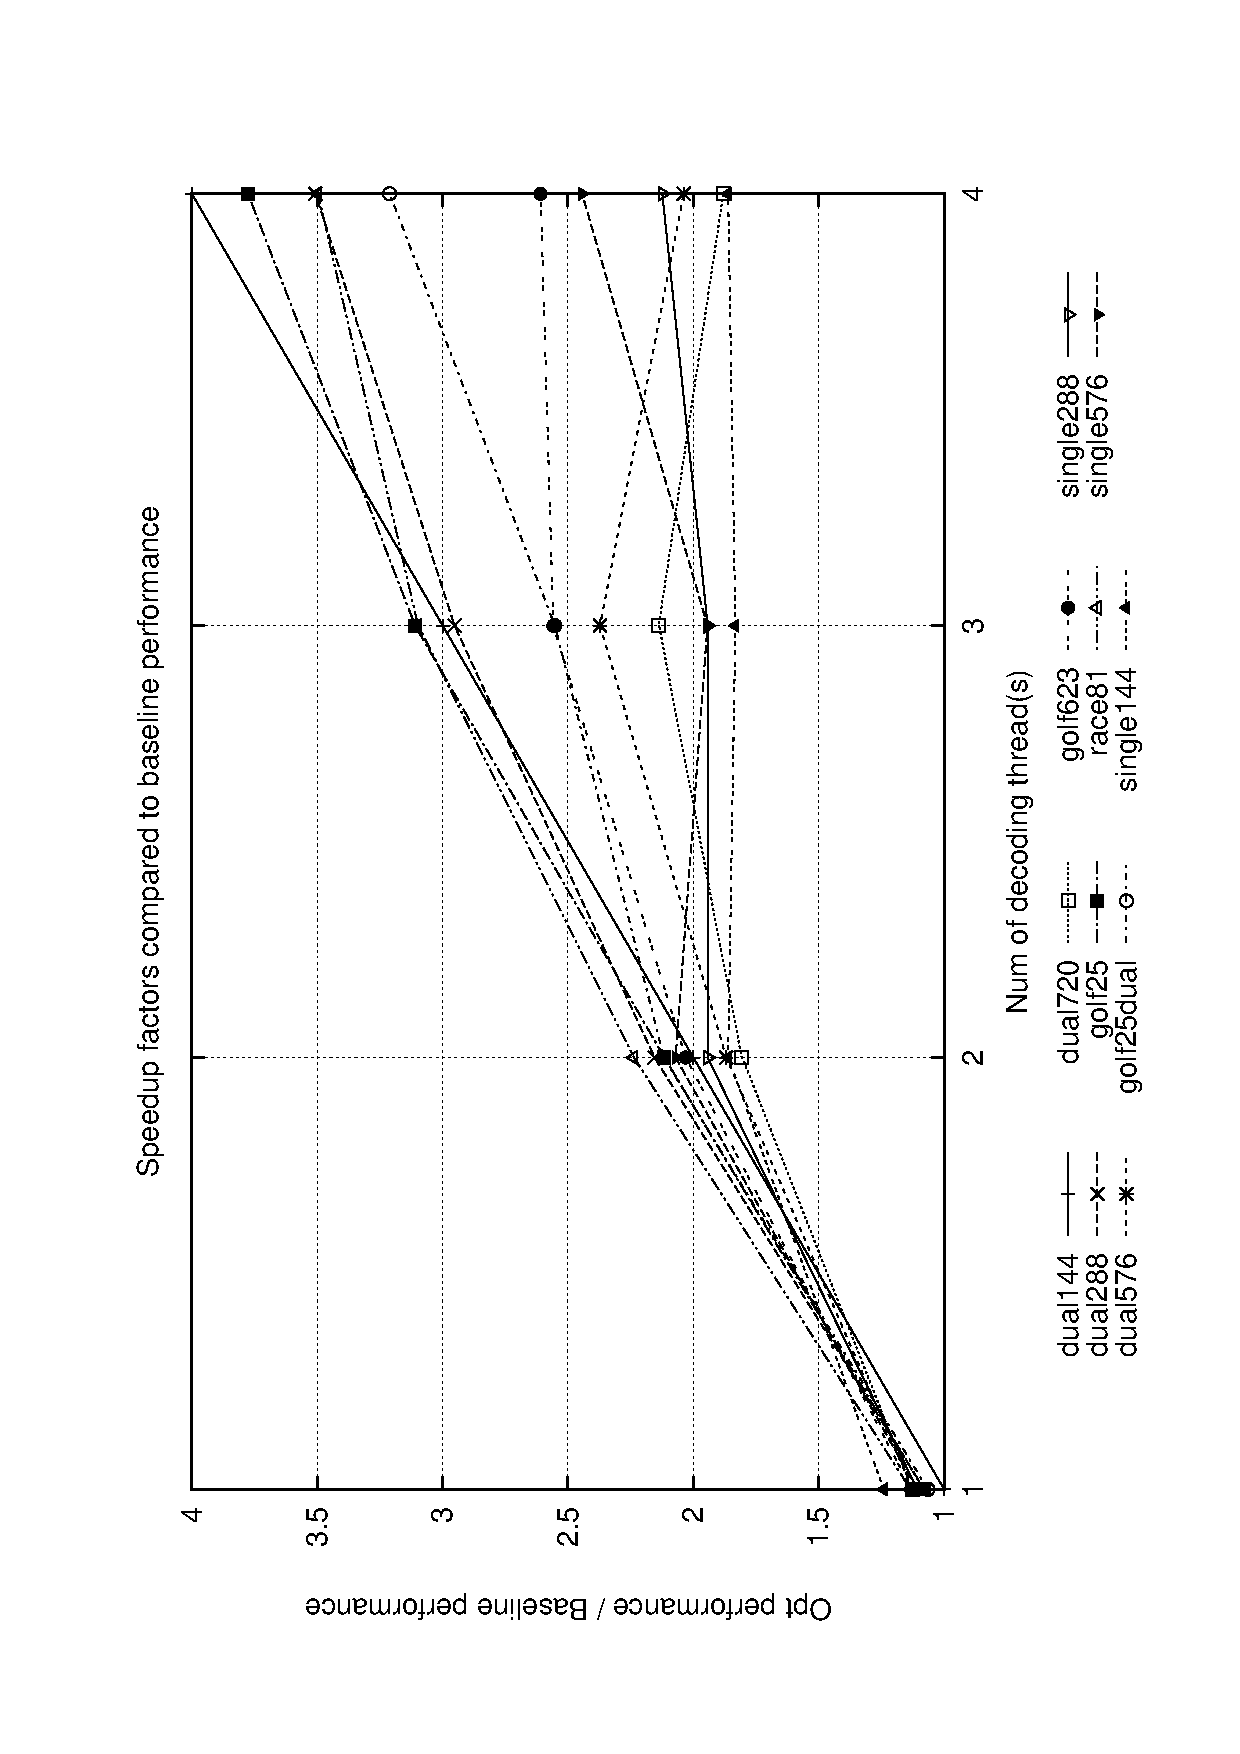
\includegraphics[height=\textwidth,angle=-90]{speedupMS}
\caption{解码不同视频的加速比(使用MS编译器)}
\label{fig:speedupMS}
\end{center}
\end{figure}


\begin{figure}[htbp]
\begin{center}
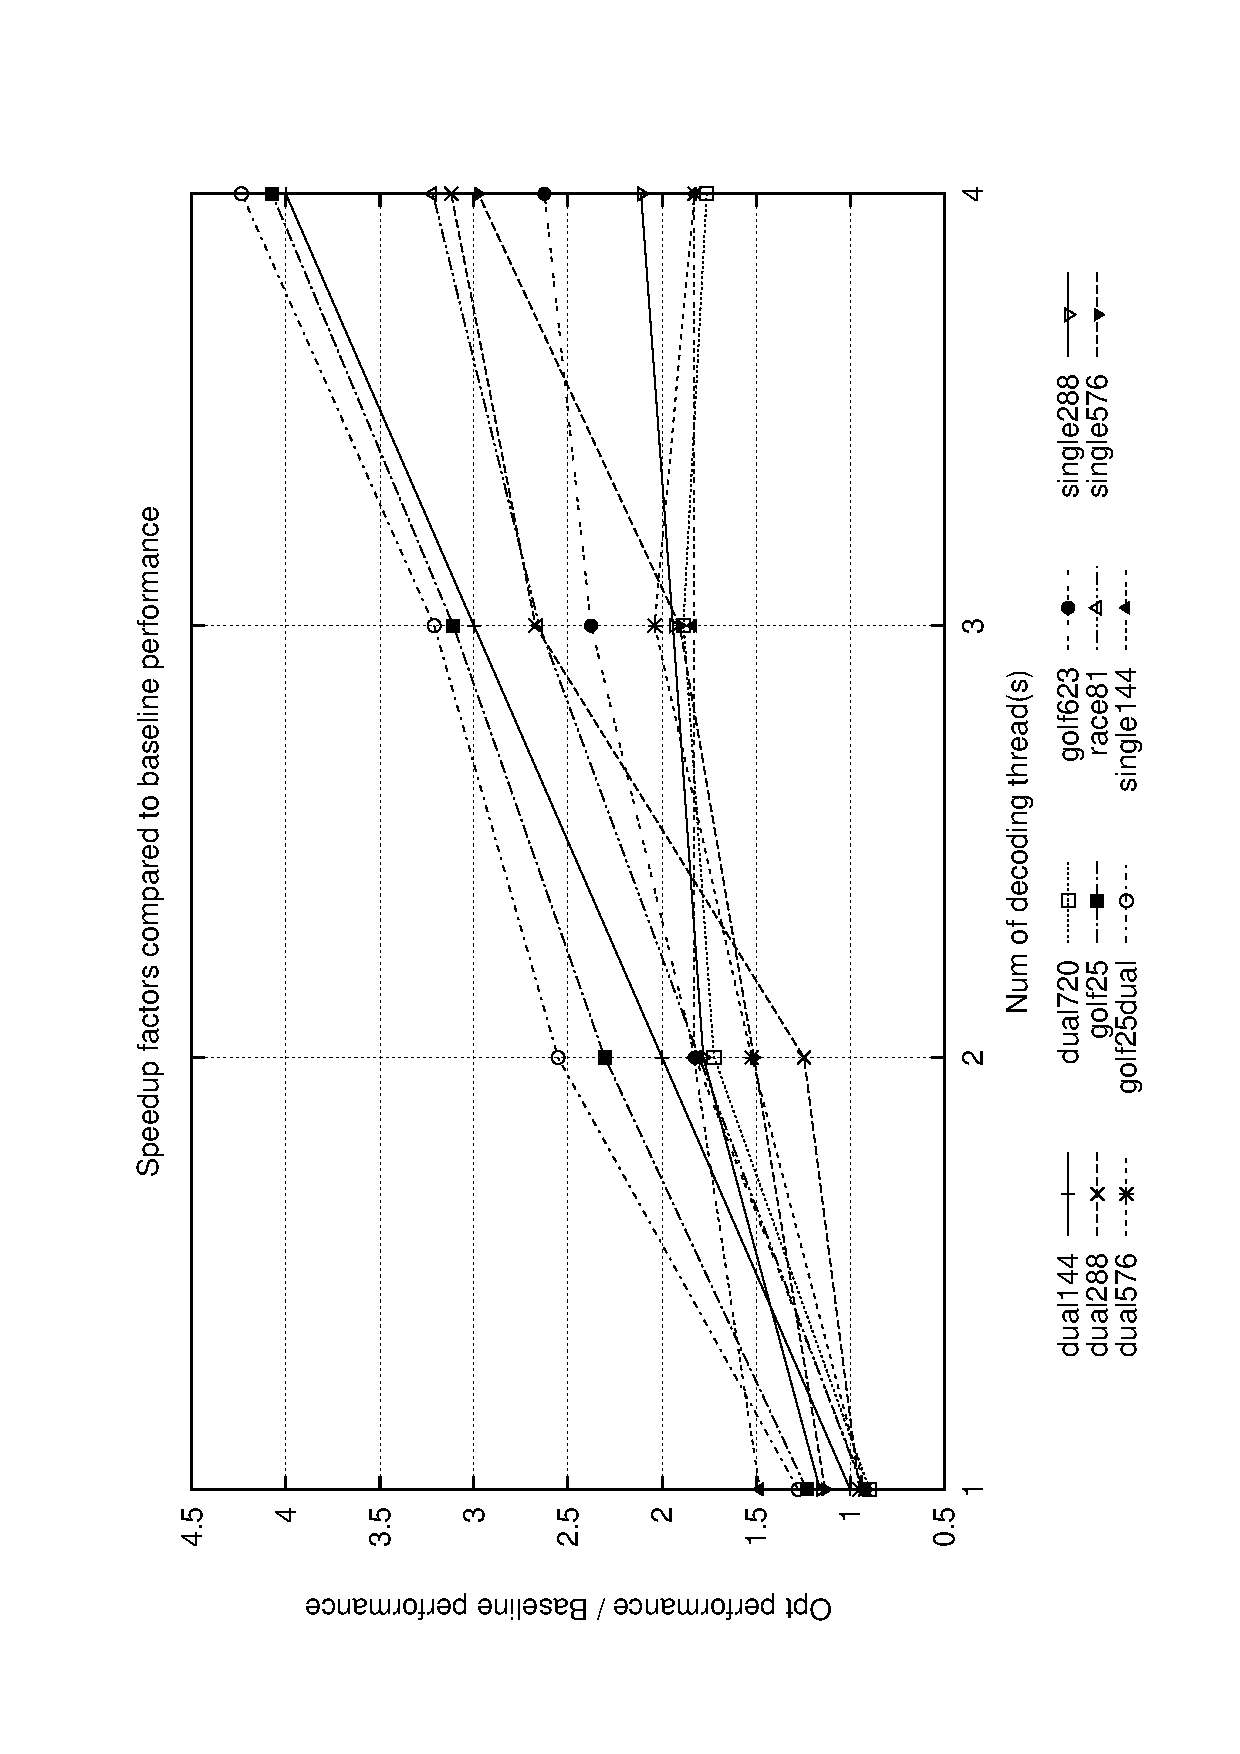
\includegraphics[height=\textwidth,angle=-90]{speedupICC}
\caption{解码不同视频的加速比(使用ICC编译器)}
\label{fig:speedupICC}
\end{center}
\end{figure}

经过优化后的解码器支持大于1的解码线程数。用Visual Studio内置的微软编译器编译的解码器用1到4个线程解码各个测试样例的性能与优化前的基准性能相比的加速比如\autoref{fig:speedupMS}所示。用ICC编译器编译的解码器的加速比如\autoref{fig:speedupICC}所示。更清晰的版本附在本章末尾的\autoref{fig:speedupMS2}和\autoref{fig:speedupICC2}。

可以看出,几条折线的趋势都证明增加线程数能够加快解码速度,而几条折线在线程数为3和4时的变化又有所不同:
\begin{itemize}
\item dual144的加速比正好为线程数,这是一个巧合。不过也能部分说明当视频的并行性足够时,增加的线程资源能够被充分利用。
\item golf25、golf25dual、dual288和race81这四个视频也能充分利用额外的资源。
\item single144、single288、single576、single720这些单路的视频加速比都没有超过2.6,这是由于一路视频的参考结构比较简单,没有视角间的参考。调度器很难安排出能够并行处理的大于2个任务。
\item golf623的加速比低于预期,我们推测原因在于编码时的GOPSize设成4对于8路视频偏小了,造成并行程度不够。
\end{itemize}


对部分测试视频的解码帧率如\autoref{fig:viewerfps}。这里计算的帧率是同时解码N路时的帧率,也就是观看者实际看到的等效帧率。对两路视频而言,要达到30fps的等效帧率,必须能够实际解码速率达到60fps。

从图中可以看到,对于实验目标针对的$720\times 576$的两路视频,只要线程数超过一个,就已经达到并超过了设定的实验目标。

\autoref{fig:viewerfps}也暴露了一个问题:当解码线程数增加时,解码性能并不是单调上升的。例如single576$_{MS}$(图中黑色实底纹数据)的测试结果在三线程时的解码性能反而低于两线程。其中的原因结合\autoref{fig:speedupMS}的相应数据可以做出如下解释:

single576$_{MS}$这段测试视频的预测结构蕴含的并行性不高,多线程解码的加速比最高仅仅达到2.2左右。这样一来,帧并行解码在线程数为3较线程数为2时增加的线程切换开销带来的性能损失大于多线程的性能提升,最终使得实际性能下降。对于四线程的情形,更多的线程使得宏块并行更加彻底,性能提升反过来超过了线程切换损失,体现为实际性能上升。

\begin{figure}[htbp]
\begin{center}
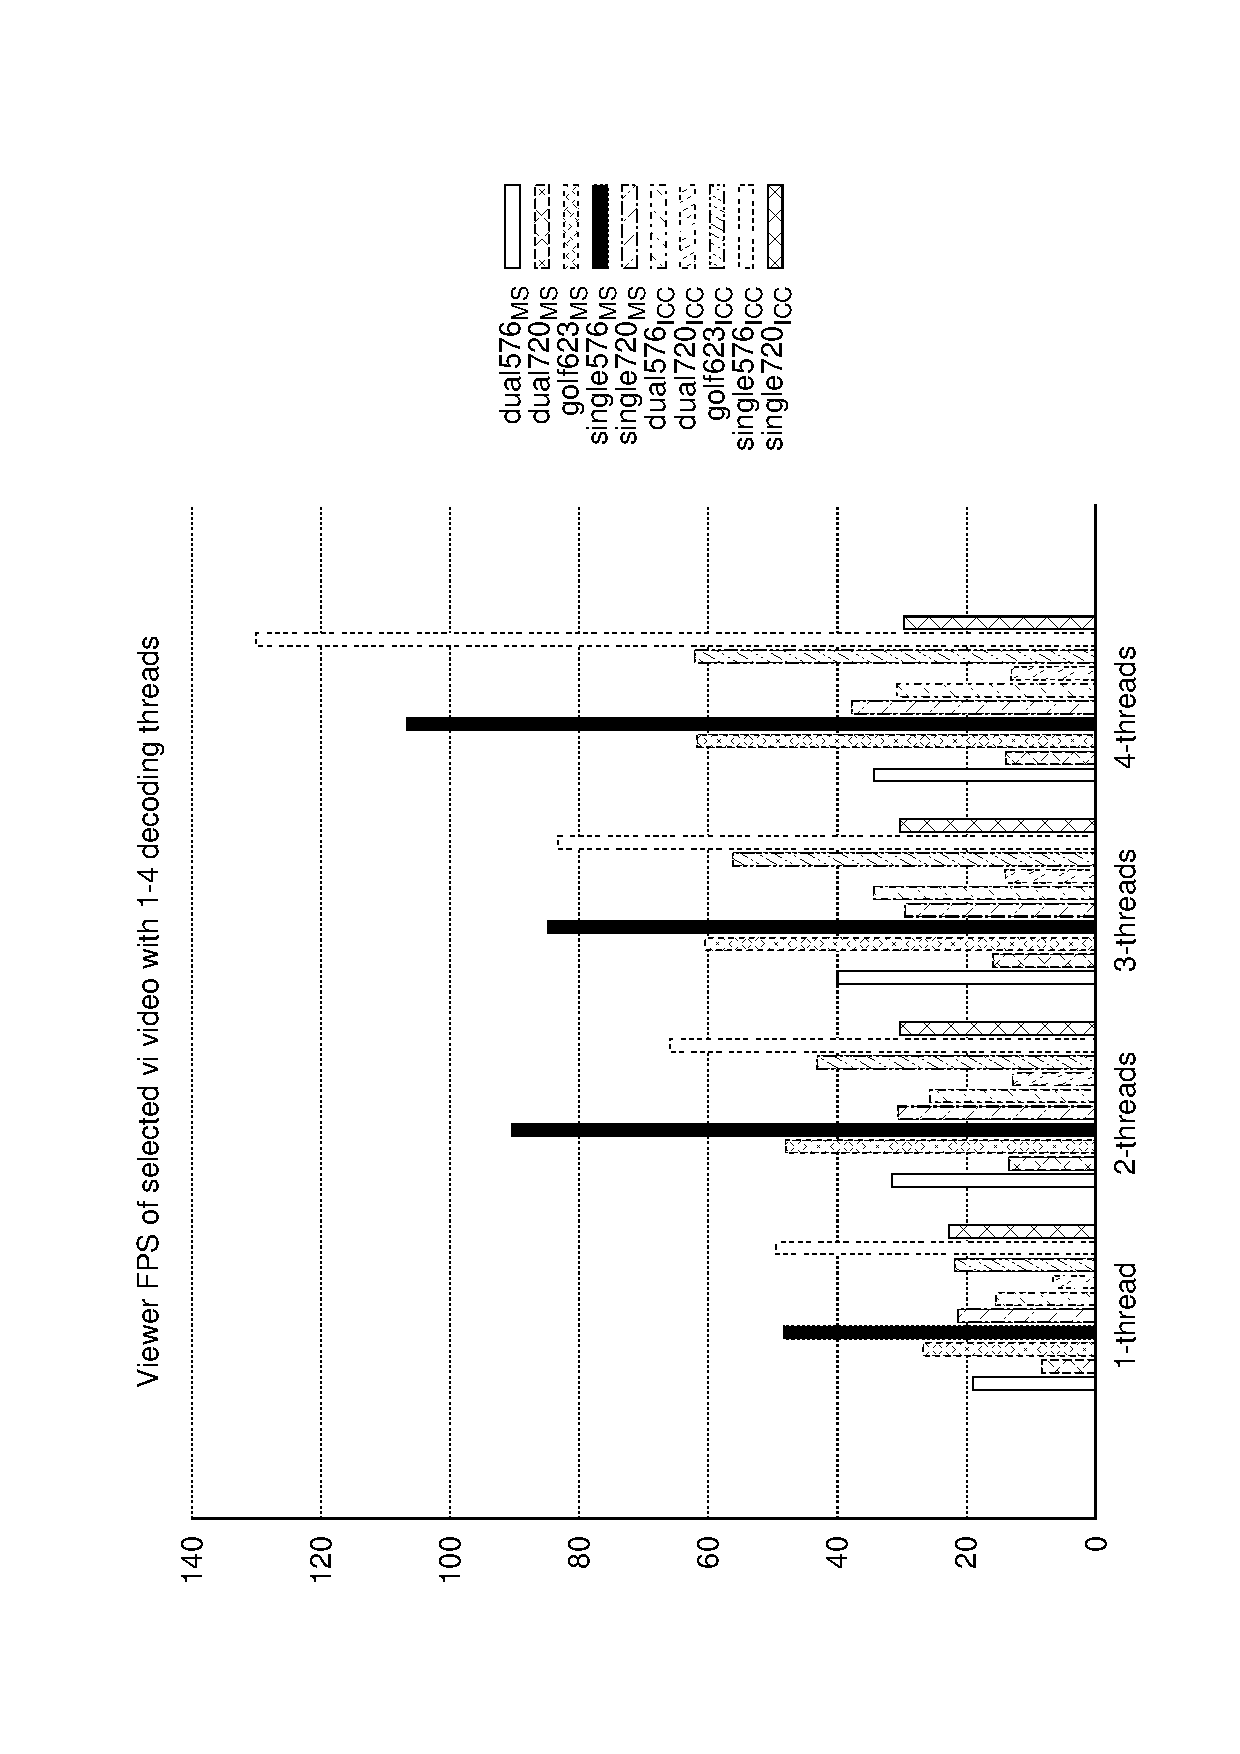
\includegraphics[width=\textwidth]{viewerfps}
\caption{部分视频解码的等效帧率}
\label{fig:viewerfps}
\end{center}
\end{figure}

\section{小结}
\label{sec:sum6}

本章详细介绍了测试解码器性能的视频准备工作,利用ffmpeg和JMVC生成了用于测试的单路、两路和八路的视频片段;利用解码器对这些视频片段进行解码,记录解码耗时,得到解码器的性能;对比了优化后与优化前的解码器性能,解码不同的测试视频得到了不同的结果,但是总的趋势是符合逻辑的{\pozhehao}当测试视频的预测结构蕴含更大的并行性时,多线程解码就能获得更高的加速比;测试数据还证明了优化后的解码器达到了先前设定的实时解码$720\times576$两路立体视频的优化目标。


\begin{figure}[htbp]
\begin{center}
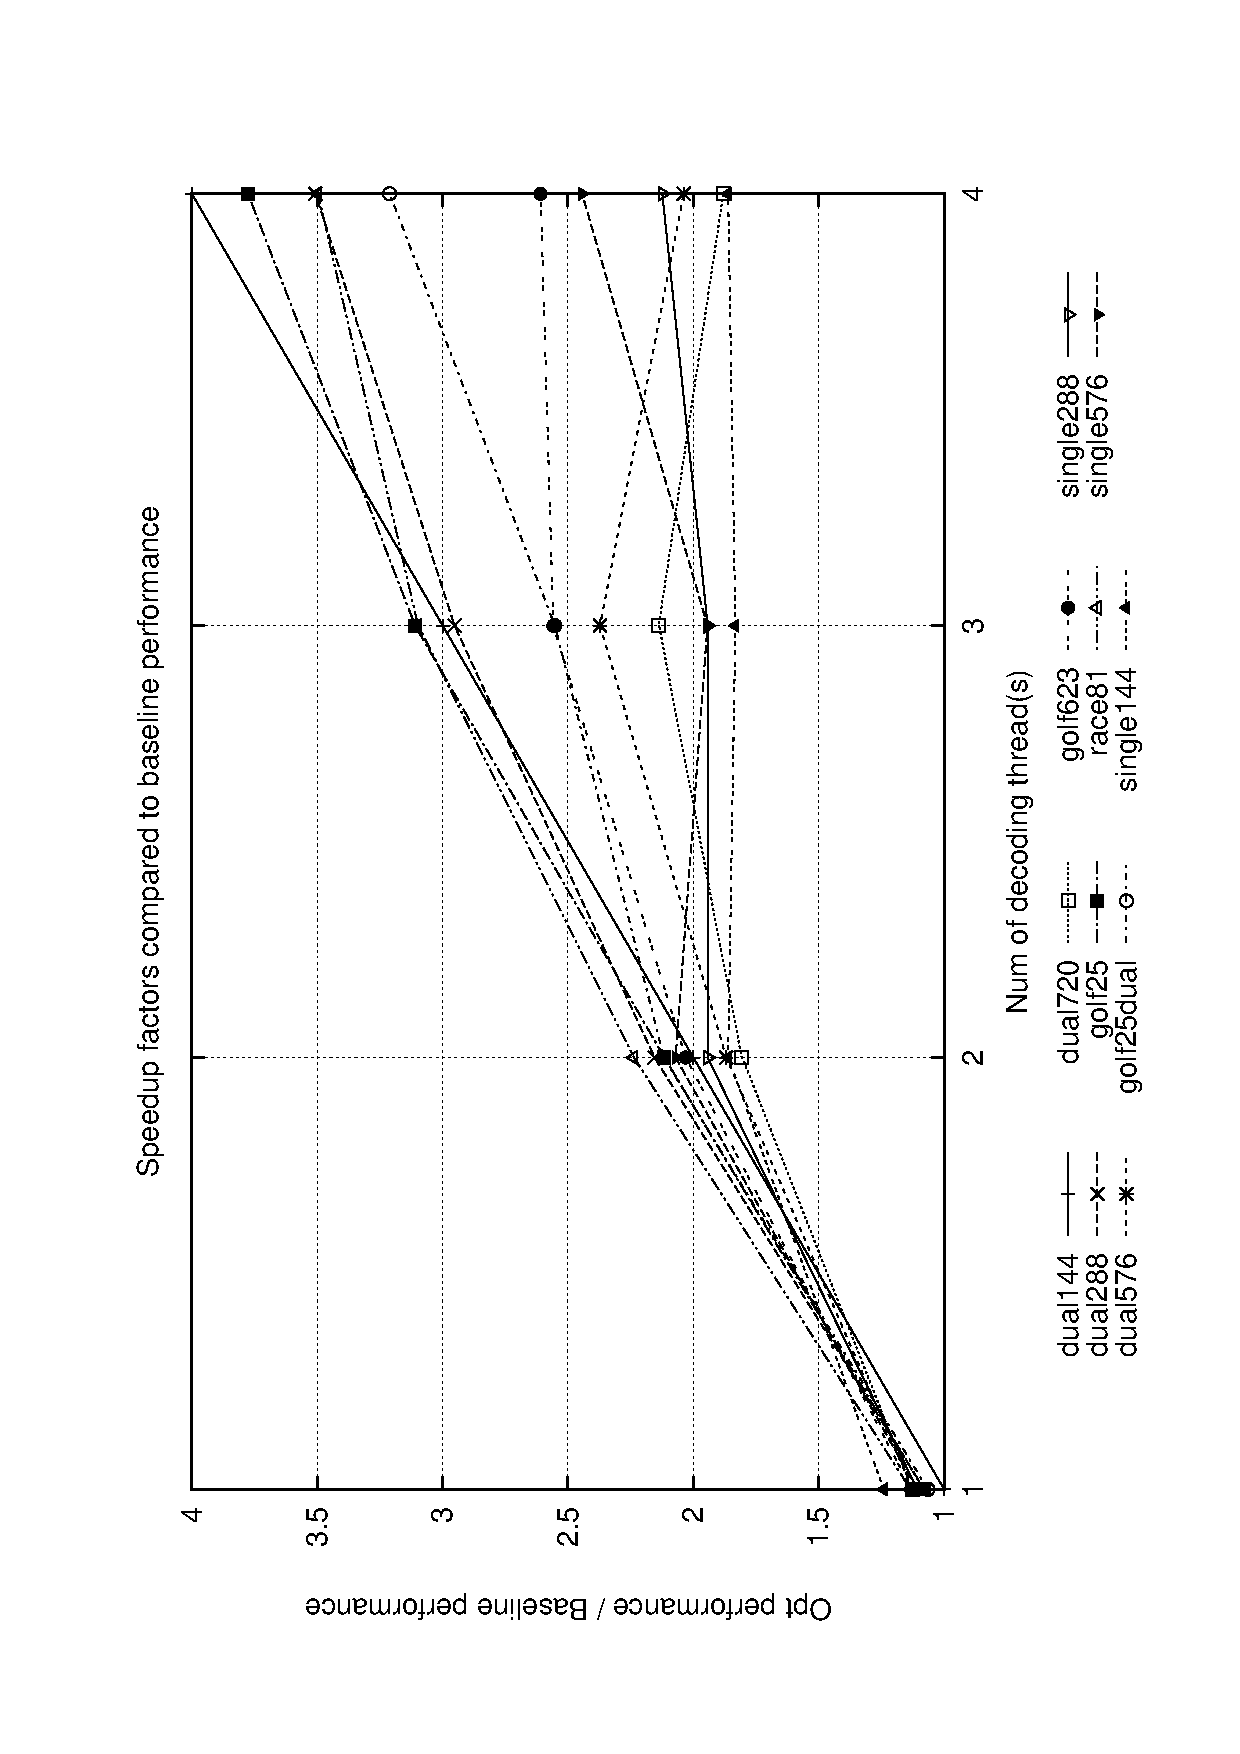
\includegraphics[width=\textwidth]{speedupMS}
\caption{解码不同视频的加速比(使用MS编译器)}
\label{fig:speedupMS2}
\end{center}
\end{figure}


\begin{figure}[htbp]
\begin{center}
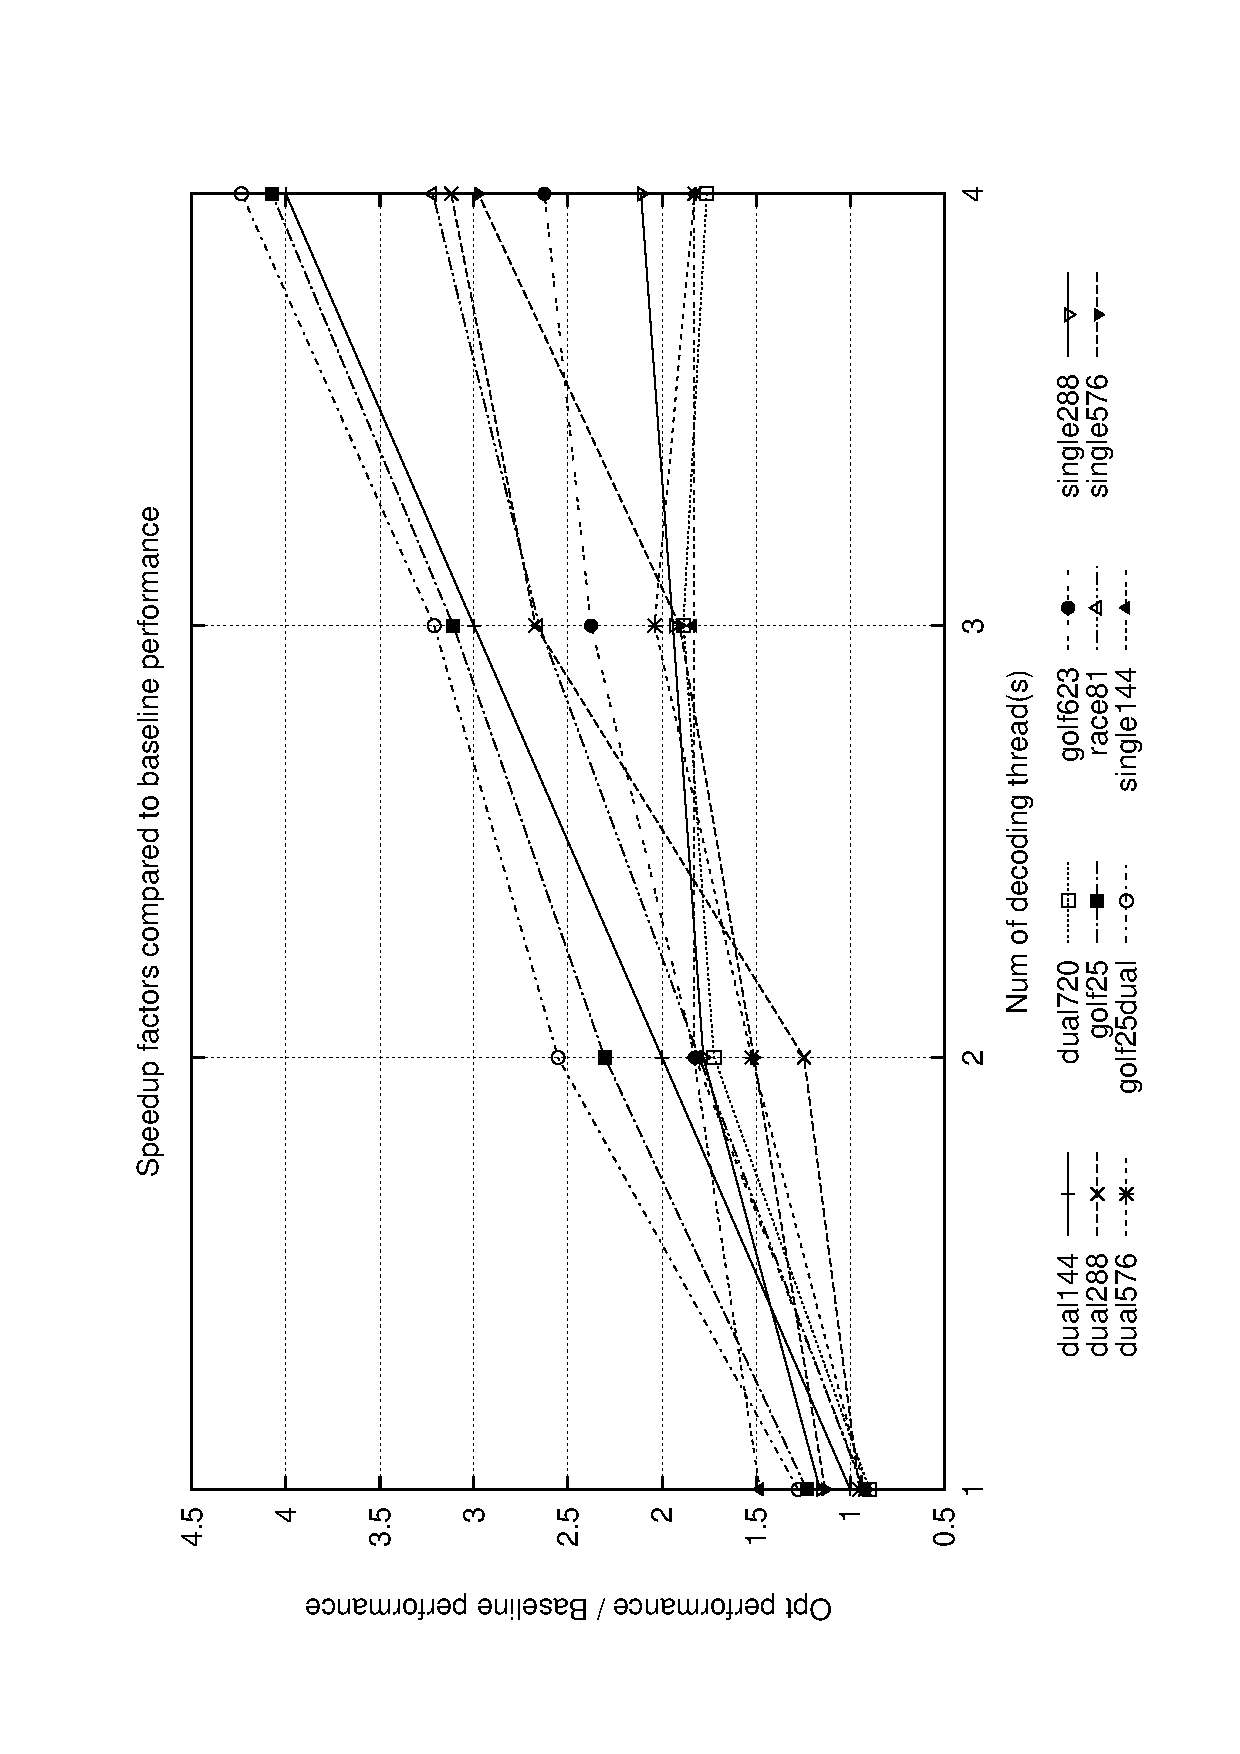
\includegraphics[width=\textwidth]{speedupICC}
\caption{解码不同视频的加速比(使用ICC编译器)}
\label{fig:speedupICC2}
\end{center}
\end{figure}


\cleardoublepage

%%% Local Variables: 
%%% mode: latex
%%% TeX-master: t
%%% End: 

\cleardoublepage

\chapter{3D播放器设计与实现}
\label{cha:3Dplayerdesignandrealization}

\section{实验平台}
\label{sec:3dplayerhardwareplatform}

%\subsection{NVIDIA 3D Vision套装介绍}
%\label{subsec:nvidia3dvisionbrief}

% 此处可以插入一段介绍以及图片

%\subsection{实验平台}
%\label{subsec:3dplayerplatform}
% 平台的介绍
我们希望利用NVIDIA 3D Vision套装进行3D播放器的立体显示。由于3D Vision只支持Windows Vista和Windows 7,所以实验的操作系统有限制。实验主要在以下环境下进行:

\begin{itemize}
\item {硬件平台}

\begin{itemize}
\item Intel Core2 Quad Q9400 @ 2.66GHz
	\footnote{SpeedStep功能关闭}
\item 4GB DDR2/800 Memory
\item NVIDIA GeForce GTS 250 with 512MB
\end{itemize}

\item {软件平台}

\begin{itemize}
\item Microsoft Windows 7 Enterprise
	\footnote{获取自:\href{http://helpdesk.tsinghua.edu.cn/yhfw/yhfw_zbrj_tz.jsp}{清华大学校园正版软件服务}}
\item NVIDIA 3D Vision Driver v1.23
\item DirectX 11.0
\item Microsoft Visual Studio 2008 SP1
	\footnote{获取自:\href{http://helpdesk.tsinghua.edu.cn/yhfw/yhfw_zbrj_tz.jsp}{清华大学校园正版软件服务}}
\end{itemize}

\end{itemize}


\section{调研阶段}
\label{sec:3Dplayersurvey}

想要实现3D播放器就需要调用硬件资源,至少要能让3D Vision的眼镜工作起来。对此,我们进行了一段时间的调研,希望找到一些资料,了解如何调用这些资源。

%nvapi

NVIDIA的3D Vision驱动盘上有一个3D播放器程序,可以用来播放NVIDIA官方网站上提供下载的一些3D视频片段。可惜这个播放器不是开源的,我们猜想其内部是利用了NVIDIA提供的API函数的,于是去NVIDIA的开发站点上下载了NVAPI\footnote{\url{http://developer.download.nvidia.com/NVAPI/NVAPI_May2009.zip}}。在NVAPI中,我们找到了和立体显示相关的部分接口函数如\autoref{lst:NVAPI}:

% 此处插入NVAPI截图
\begin{lstlisting}[caption = {NVAPI中立体显示的部分函数}, label = lst:NVAPI]
`\dots`
NVAPI_INTERFACE NvAPI_Stereo_Enable(void);
NVAPI_INTERFACE NvAPI_Stereo_Disable(void);
NVAPI_INTERFACE NvAPI_Stereo_CreateHandleFromIUnknown(IUnknown *pDevice, StereoHandle *pStereoHandle);
NVAPI_INTERFACE NvAPI_Stereo_Activate(StereoHandle stereoHandle);
NVAPI_INTERFACE NvAPI_Stereo_Deactivate(StereoHandle stereoHandle);
NVAPI_INTERFACE NvAPI_Stereo_CaptureJpegImage(StereoHandle stereoHandle, NvU32 quality);
`\dots`
\end{lstlisting}

其中的确有Stereoscopic3D子项,但是只有一些状态查询、保存当前图像等函数,并没有我们所需要的能够实现在显示图像或图形时能控制3D眼镜开启的接口。对此,我们认为是public版本的NVAPI不完整,没有包含这部分比较新的接口。我们尝试了注册NVIDIA的注册开发人员\footnote{\url{http://developer.nvidia.com/page/registered_developer_program.html}}(registered developer),期望能够获得完整版的NVAPI,但是申请一直没有得到答复。这个方向的调研到此中断。

%manual inter-view display

由于3D Vision的原理是将左右两个视点的图像交替显示,然后通过同步器控制眼镜快门使得每个时刻都只有一只眼睛能看到为其显示的图像,以此来实现双目立体显示。而在NVAPI中,我们又发现了名为NvAPI\_Stereo\_Enable()和NvAPI\_Stereo\_Activate()的两个函数,继而提出了一个问题:如果我们人工地控制程序交替显示两个视点的视频,显式地调用这两个函数(或其中之一),NVIDIA的驱动能否自动地让3D眼镜工作?

我们为此写了一个测试程序,可惜结果并不令人满意,我们看到的就是交替渲染的有重影的图像,而3D眼镜根本没有工作。

%d3d - cube demo

我们一直在NVIDIA的开发人员论坛以及各类3D相关的开发论坛上不断寻找关于3D Vision调用的尝试。尽管NVIDIA的开发人员论坛上有十几个活跃的thread是与此相关的,但是长期以来没有人回复可行的解决方案。经过一段时间的搜索,我们终于在mtbs3d.com上找到了一个帖子\footnote{\href{http://www.mtbs3d.com/phpBB/viewtopic.php?f=7&t=5072}{http://www.mtbs3d.com/phpBB/viewtopic.php?f=7\&t=5072}}声称成功地调用3D Vision显示了立体图像。有人根据该贴的说明进行了尝试表示同样获得成功,并给出了一个Demo,显示一些在屏幕上进行XYZ三个方向上平移的立方体。我们下载了该Demo程序编译运行证实可行。这个Demo是基于Direct3D的,其中没有明文调用NVIDIA的API,所以我们认为:NVIDIA的驱动对Direct3D程序能够自动启用3D眼镜。

\section{3D播放器设计}
\label{sec:3dplayerdesign}

\subsection{静态3D图像的显示}
\label{subsec:static3dimgdisp}

\begin{figure}
\begin{minipage}{0.5\textwidth}
	\centering
	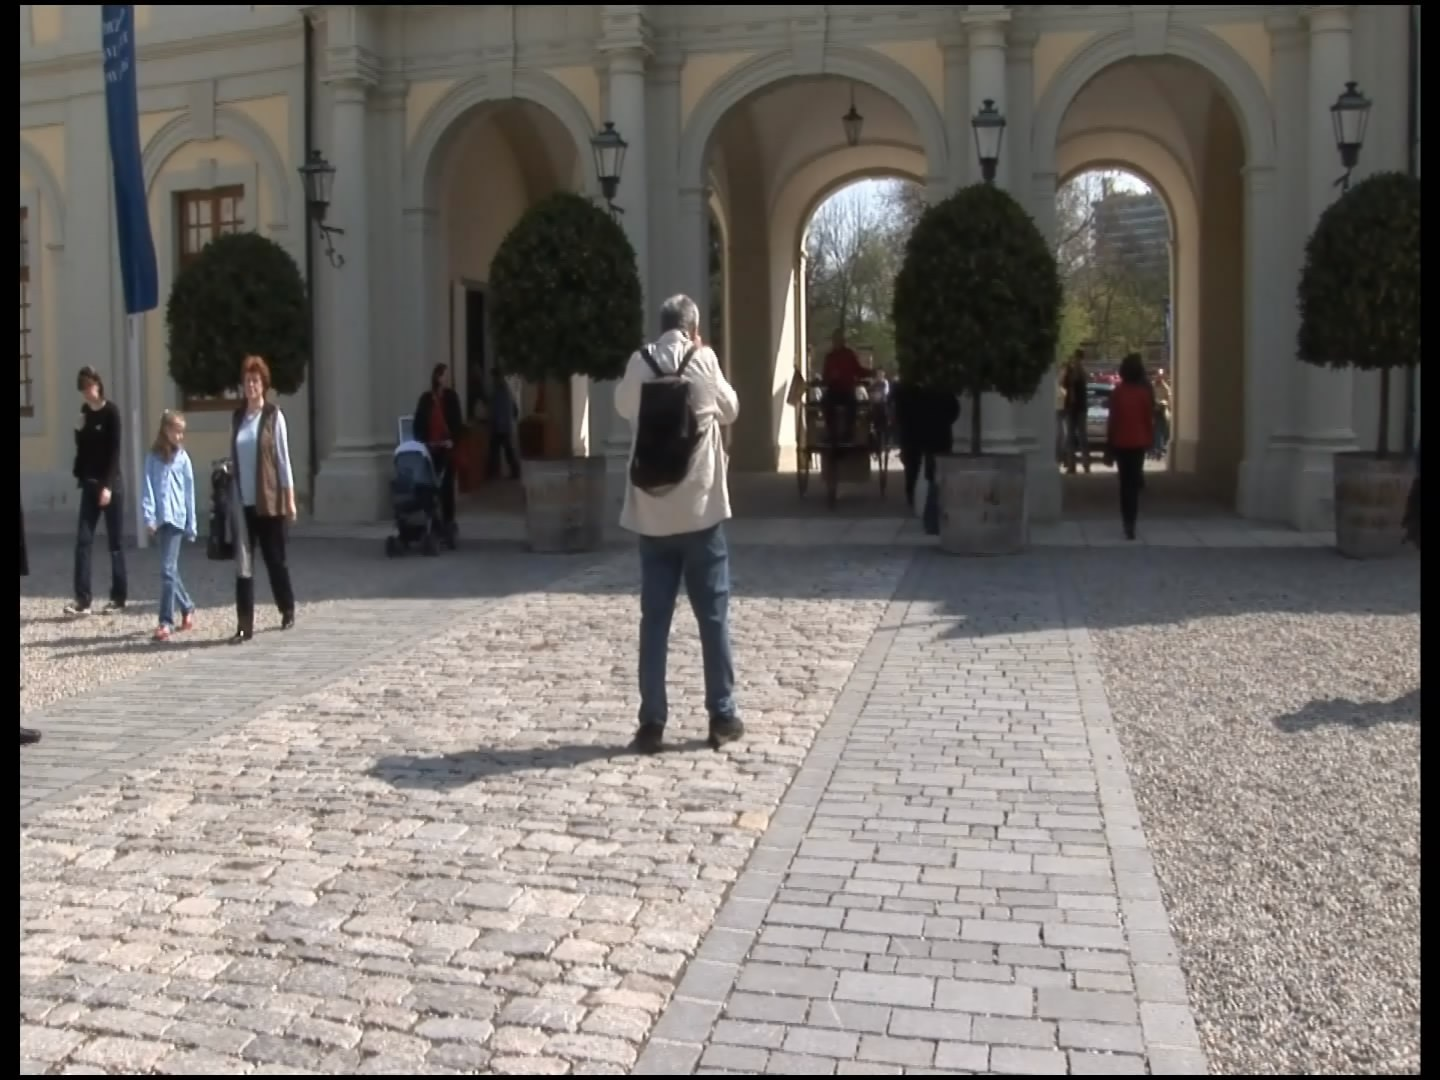
\includegraphics[width=0.95\textwidth]{staticLeftView.jpg}
	\caption{静态3D显示测试的左眼图像}
	\label{fig:staticleftview}
\end{minipage}\hfill
\begin{minipage}{0.5\textwidth}
	\centering
	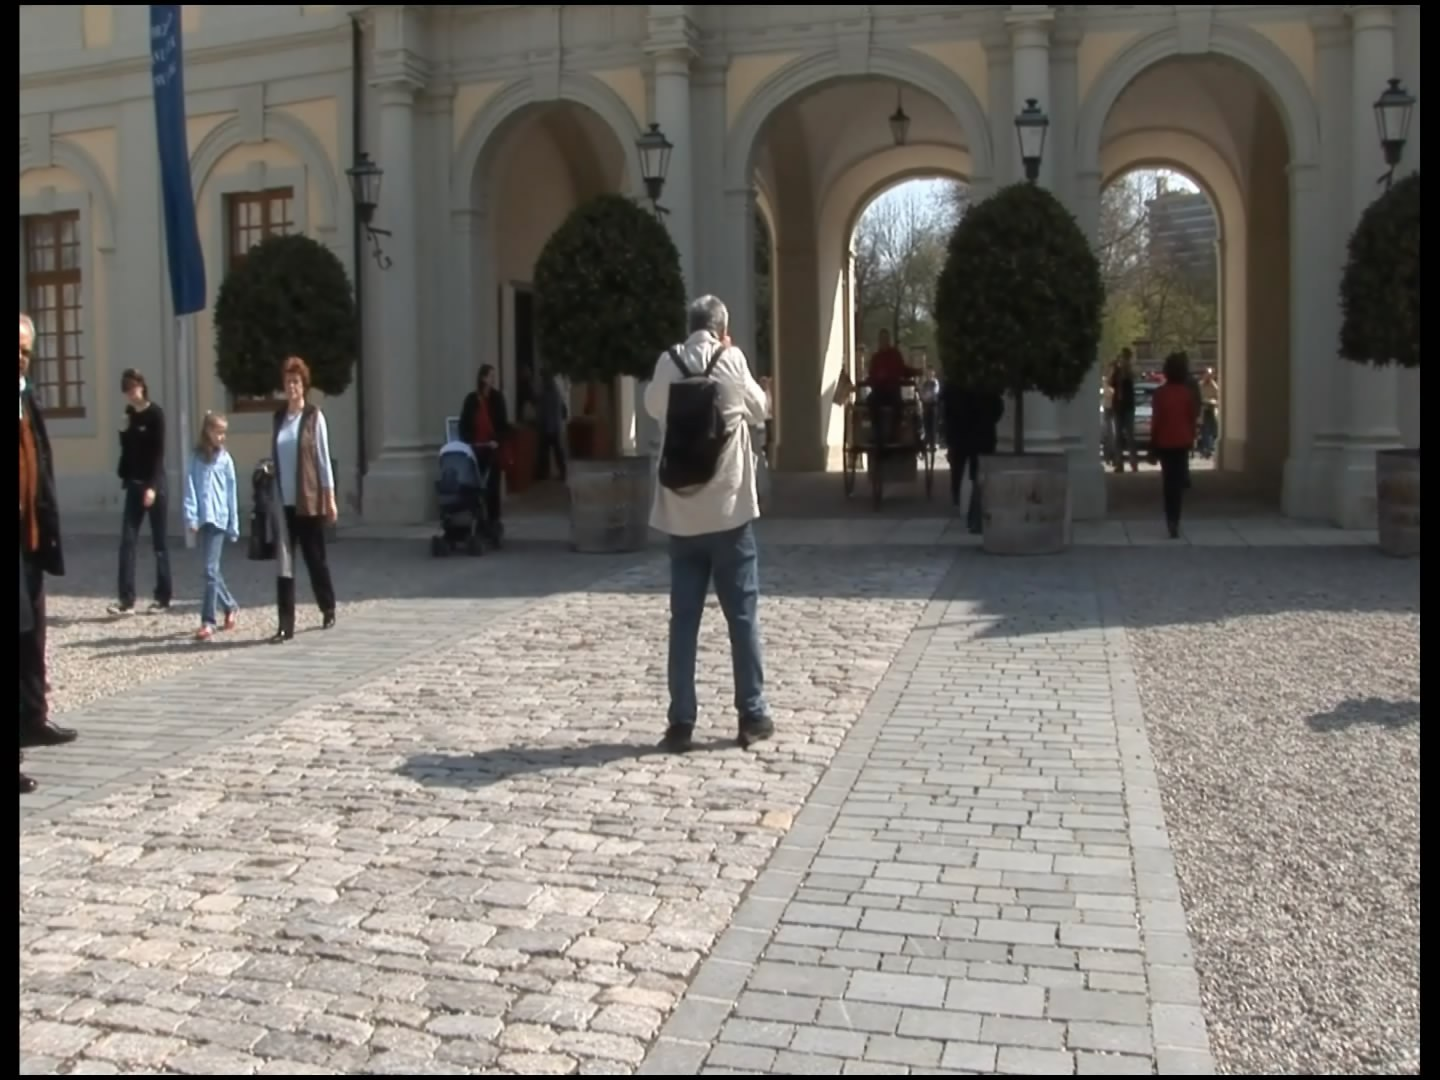
\includegraphics[width=0.95\textwidth]{staticRightView.jpg}
	\caption{静态3D显示测试的右眼图像}
	\label{fig:staticrightview}
\end{minipage}
%\caption{用于静态3D显示测试的图像}
%\label{fig:staticview}
\end{figure}

有了一次成功调用3D眼镜的经历,我们找到了一些头绪,并就此开始设计3D播放器。

我们希望3D播放器能够接收一系列的图像,这些图像分为两个序列,分别是左眼和右眼视角的图像。然后播放器以一个预设的帧率交替播放这两个序列中的图像。如果NVIDIA的驱动能够成功开启3D眼镜,此时我们通过3D眼镜就能看到立体图像了。

经过不断尝试,我们终于实现了一帧静态3D图像的显示。做法如下:

\begin{enumerate}
\item 首先我们创建一个IDirect3DSurface9,这是Direct3D中用于渲染的表面。假设我们要显示的图像的宽度和高度分别为$imgWidth$和$imgHeight$。这个表面的宽度就应该是$2\times imgWidth$,这一点较容易理解,因为有左右两个视角的图像。但是这个表面的高度必须设为$imgHeight+1$,这个多出来的1像素是上文提及的帖子中指出的关键点之一,算是一个magic number。实验中我们把高度设为$imgHeight$得到的就不是立体图,而是两幅横向并列显示的拉伸过的图像。
\item 有了这个表面之后,我们需要为其添加内容。以左上角$(0,0)$为原点,调用D3DXLoadSurfaceFromFile()读入左眼图像(\autoref{fig:staticleftview}),再以$(imgWidth,0)$为原点再次调用函数读入右眼图像(\autoref{fig:staticrightview})。
\item 在渲染之前,我们还要为这个待显示的结构写一个头,叫做$LPNVSTEREOIMAGEHEADER$,其中要指定宽度、高度、颜色深度以及一个singature,这个名为$NVSTEREO\_IMAGE\_SIGNATURE$的signature需要赋一个特定的值0x4433564e。见\autoref{lst:LPNVSTEREOIMAGEHEADER}。
\begin{lstlisting}[caption = {LPNVSTEREOIMAGEHEADER的结构}, label = lst:LPNVSTEREOIMAGEHEADER]
// Stereo Blitdefines
#define NVSTEREO_IMAGE_SIGNATURE 0x4433564e //NV3D
typedef struct _Nv_Stereo_Image_Header {
    unsigned int dwSignature;
    unsigned int dwWidth;
    unsigned int dwHeight;
    unsigned int dwBPP;
    unsigned int dwFlags;
} NVSTEREOIMAGEHEADER, *LPNVSTEREOIMAGEHEADER;
\end{lstlisting}
\item 经过如上的操作,利用Direct3D的renderer渲染输出到显示器的图像就是立体图了(\autoref{fig:staticdualview})。注意实际透过眼镜是看不到重影的,两帧图像交替显示,眼镜快门相应地轮流遮挡视线,只能看到各自视角的图像。
\end{enumerate}


\begin{figure}[htbp]
\begin{center}
\includegraphics[width=0.9\textwidth]{staticDualView.pdf}
\caption{渲染后输出的3D图像}
\label{fig:staticdualview}
\end{center}
\end{figure}

实现了一帧静态立体图的显示,就有了显示立体视频的基础,显示动态图像的部分在下一节阐述。

\subsection{立体视频(图像序列)的显示}
\label{subsec:motion3dimgdisp}

视频的显示可以看做以一个预设的帧率FPS(frames per second)显示一个图像序列中的一张张图像。这里的帧率根据视频的制式不同而改变,一般都在24或30左右。

视频中的FPS与游戏中的FPS有所不同。在游戏中,往往追求硬件所能处理的最高的FPS,尽可能使画面更加流畅。而在视频回放的时候,有一个固定的帧率,必须要尽可能让实际帧率接近这个预设的帧率,才能满足视频的每一帧出现在时间轴的正确位置上。然而,视频播放和游戏的渲染又有一个共同点,当硬件资源很有限的情况下,会将帧率降到很低,出现跳帧,这也是为了保证画面的时间正确性,避免出现像“慢动作回放”一样的效果。

综合以上的特点,我们就需要有一个控制帧率上限的机制,保证帧率在资源足够的时候不会超过预设值;同时要支持在资源受限时自动跳帧。

为了实现这样的机制,我们需要获得较为精确的时间,来控制每一帧持续的时长。ANSI C++中提供的getTicker()函数是ms级的,比较粗糙,无法满足一些常见的(如23.97)标准帧率的控制需要。对此,我们查阅了MSDN的文档后选用了Windows API中提供的QueryPerformanceCounter()和QueryPerformanceFrequency()配合实现us级的计时器。

我们实现的帧率上限控制的机制如下:在开始播放第0帧的时刻记下当前时间$t_{0}$。在渲染完第$i$帧$F_{i}$之后,获得当前时间$t_{n}$,然后准备进行第$(t_{n}-t_{0})\times FPS$的渲染。通过比较当前已渲染的帧$F_{i}$和待渲染的帧$F_{n}$是否一致来决定是否进行渲染操作。这个机制的核心就是\autoref{eqn:Fn}。
\begin{equation}\label{eqn:Fn}
F_{n}=(t_{n}-t_{0})\times FPS
\end{equation}
其中$FPS$为根据播放内容而预设的一个帧率,$t_{n}$为当前时刻,$t_{0}$为播放视频第0帧的起始时刻,$F_{n}$为当前时刻应该渲染的帧的序号。

帧率上限控制算法的伪代码见\autoref{algo:frameratecap}。

\begin{algorithm}
\caption{Frame rate cap}
\label{algo:frameratecap}
\begin{algorithmic}[1]
	\STATE $\_start \Leftarrow initialTime$ %\COMMENT{store the initial time}
	\STATE $bufferd = FALSE$
	\STATE $lastRenderedFrame \Leftarrow -1$
	\WHILE{$TRUE$}
		\STATE $\_current \Leftarrow currentTime - \_start$ %\COMMENT{get elapsed time}
		\STATE $frameToRender \Leftarrow \_current * FPS$ %\COMMENT{calc the frame to render}
		\IF{$frameToRender + 1> totalFrames$}
			\STATE $break$ \COMMENT{break when reaching the last frame}
		\ENDIF
		\IF{$buffered = FALSE$}
			\STATE load $Frame_{frameToRender+1}$ to memory
			\STATE $buffered \Leftarrow TRUE$
		\ENDIF
		\IF{$frameToRender \neq lastRenderedFrame$}
			\STATE render $Frame_{frameToRender}$
			\STATE $lastRendered \Leftarrow frameToRender$
			\STATE $buffered \Leftarrow FALSE$
		\ENDIF
	\ENDWHILE
\end{algorithmic}
\end{algorithm}

\section{播放器测试}
\label{sec:3dplayerdemo}

%功能
我们实现的播放器具有如下功能:
\begin{description}
\item[输入] 左右两个视点的图像序列文件名格式。实验中采用了“前缀+序号+后缀”的方式。前缀为文件相对路径,图像的文件名包含其对应的帧序号,后缀为文件扩展名。\\
	图像序列的总帧数$totalFrames$,见\autoref{algo:frameratecap}的第7行。\\
	播放时的帧率$FPS$,见\autoref{algo:frameratecap}的第6行。
\item[输出] 在显示器上输出如\autoref{fig:staticdualview}效果的立体图序列,帧率为$FPS$。通过3D眼镜可以看到立体视频。
\end{description}

%瓶颈

我们使用$720\times576$的分辨率对播放器进行测试,选用了几段不同的图像序列。在不断测试过程中,我们发现在图像包含告诉运动的物体时能够看出跳帧现象。于是我们输出了每一帧的load和render情况,发现实际帧率在19fps到21fps不等。我们希望寻找性能瓶颈所在,进行了以下排查:
\begin{itemize}
\item 我们首先考虑是否因为图像序列的格式为JPEG,在读取的时候需要时间解码。于是将图像序列转化为BMP格式的位图,测试发现帧率进一步降至14fps左右。测试用图存为JPEG时每帧平均大小50KB,BMP则超过300KB。
\item 有了JPEG和BMP的对比,我们认为磁盘I/O可能是一个瓶颈。对此,我们划分了500MB的内存作为一个RAMDISK。用HD Tune测试这个分区的读写速度和随机访问时间等指标如下:
\begin{description}
\item[Transfer Rate (Min)] 2751.7MB/sec
\item[Transfer Rate (Max)] 3363.2MB/sec
\item[Transfer Rate (Avg)] 3239.8MB/sec
\item[Access Time (Avg)] 0.0ms
%\item[Burst Rate] 3670.7MB/sec
%\item[CPU Usage] 0.0\%
\end{description}
将图像序列存放在该RAMDISK分区上再次进行测试,帧率依然在21fps左右。所以磁盘IO被排除在瓶颈之外。
\item 此时我们决定用性能分析工具分析我们的程序,找出其中时间耗费最多的部分,将该部分打散成多个小的函数再次分析。如此循环了几次,终于找到性能瓶颈所在:我们调用D3D中的D3DXLoadSurfaceFromFile()函数两次,分别将左右眼的图像绘制到渲染的表面上。而这两个函数调用占用了整个程序运行总时间的95\%以上。
\end{itemize}
这个API的性能我们暂时未解决,尚在寻找可行的替代方法。


\section{小结}
\label{sec:sum7}

本章介绍了3D播放器设计实现的全部过程,从调研阶段遇到的各种问题、种种尝试,到发现一种可能的解决方案,然后经过一些尝试,最终借助Direct3D实现了支持3D Vision套装的立体视频播放器。不过依然存在一定的性能瓶颈,有待进一步解决。




%%% Local Variables: 
%%% mode: latex
%%% TeX-master: t
%%% End: 

\chapter{结论和展望}
\label{cha:conclusionandforesight}

\section{本文工作总结}
\label{sec:conclusion}
视频编解码的并行在近几年CPU向多核方向发展之后成为一个热门的研究领域。最近成为标准的多视点视频由于其数据量庞大、解码运算复杂,很难依靠单核的处理器达到实用的解码速度。多核并行解码多视点视频势在必行。我们以现有的多视点视频解码器为基础,希望通过一定的优化和并行处理,使普通的PC能够进行立体视频的实时解码。

%优化结果评价
总体来说,目前达到了实验初期预定的性能优化目标。通过对解码器函数级的优化,包括函数逻辑、减少循环内部的计算量、使用汇编实现部分函数,以及一个可以稳定运行的并行解码框架的实现,最终使得多视点视频的解码可以在主流PC上实现两路标清的实时解码。

%应用价值
在解码器达到性能要求之后,我们着手设计实现了一个基于NVIDIA 3D Vision套装的立体视频播放器,播放两路立体视频时能够通过3D眼镜看到立体效果。

\section{存在的问题}
\label{sec:probremained}

目前的解码器主要存在以下问题:
\begin{enumerate}
\item 多线程解码视频时的加速比不够稳定。对于部分视频会出先增加线程反而降低解码性能的情形。
\item 对MVC标准的支持尚不完整。
\item 对一些裸眼立体显示设备要求的八路视频解码性能还达不到实时。
\end{enumerate}

3D播放器主要存在以下问题:
\begin{enumerate}
\item 播放的图像序列以磁盘文件而非内存中一段数据的形式存在,将来可能成为性能瓶颈。
\item 播放时的帧率达不到流畅观看的要求,这主要是使用的一个D3D API函数调用造成的瓶颈。
\end{enumerate}


\section{未来工作}
\label{sec:futurework}

%未来继续优化方案
针对前文提出的问题,解码器在将来还需要进行以下工作:
\begin{enumerate}
\item 对于加速比反常下降的视频,我们希望实现一个智能的判断机制,在不超过线程上限的范围内,自动使用性能最优的线程数进行解码,避免性能损失。
\item 增加对MVC标准中Main Profile和Stereo High Profile的支持,增强解码器的通用性。
\item 借助GPU进行部分计算,实现两路高清视频的实时解码和八路视频的实时解码。
\end{enumerate}

3D播放器尚需要实现以下改进:
%性能提升
%接口标准
\begin{enumerate}
\item 自行实现对渲染表面的填充函数,替换D3D API调用,突破现有的性能瓶颈,保证播放的画面流畅。
\item 对播放器的输入进行修改,使其满足一个自定义的接口,方便将播放器和解码器的输出对接,做到实时解码并播放。
\end{enumerate}

\cleardoublepage
%
%%% Local Variables:
%%% mode: latex
%%% TeX-master: t
%%% End:

\chapter{带 English 的标题}
\label{cha:sampleintro}

这是 \thuthesis{} 的示例文档,基本上覆盖了模板中所有格式的设置。建议大家在使用模
板之前,除了阅读《\thuthesis{}用户手册》,这个示例文档也最好能看一看。

小老鼠偷吃热凉粉;短长虫环绕矮高粱。\footnote{韩愈(768-824),字退之,河南河阳(
  今河南孟县)人,自称郡望昌黎,世称韩昌黎。幼孤贫刻苦好学,德宗贞元八年进士。曾
  任监察御史,因上疏请免关中赋役,贬为阳山县令。后随宰相裴度平定淮西迁刑部侍郎,
  又因上表谏迎佛骨,贬潮州刺史。做过吏部侍郎,死谥文公,故世称韩吏部、韩文公。是
  唐代古文运动领袖,与柳宗元合称韩柳。诗力求险怪新奇,雄浑重气势。}


\section{封面相关}
封面的例子请参看 cover.tex。主要符号表参看 denation.tex,附录和个人简历分别参看 appendix01.tex
和 resume.tex。里面的命令都非常简单,一看即会。\footnote{你说还是看不懂?怎么会呢?}

\section{字体命令}
\label{sec:first}

苏轼(1037-1101),北宋文学家、书画家。字子瞻,号东坡居士,眉州眉山(今属四川)人
。苏洵子。嘉佑进士。神宗时曾任祠部员外郎,因反对王安石新法而求外职,任杭州通判,
知密州、徐州、湖州。后以作诗“谤讪朝廷”罪贬黄州。哲宗时任翰林学士,曾出知杭州、
颖州等,官至礼部尚书。后又贬谪惠州、儋州。北还后第二年病死常州。南宋时追谥文忠。
与父洵弟辙,合称“三苏”。在政治上属于旧党,但也有改革弊政的要求。其文汪洋恣肆,
明白畅达,为“唐宋八大家”之一。  其诗清新豪健,善用夸张比喻,在艺术表现方面独具
风格。少数诗篇也能反映民间疾苦,指责统治者的奢侈骄纵。词开豪放一派,对后代很有影
响。《念奴娇·赤壁怀古》、《水调歌头·丙辰中秋》传诵甚广。

{\kai 坡仙擅长行书、楷书,取法李邕、徐浩、颜真卿、杨凝式,而能自创新意。用笔丰腴
  跌宕,有天真烂漫之趣。与蔡襄、黄庭坚、米芾并称“宋四家”。能画竹,学文同,也喜
  作枯木怪石。论画主张“神似”,认为“论画以形似,见与儿童邻”;高度评价“诗中有
  画,画中有诗”的艺术造诣。诗文有《东坡七集》等。存世书迹有《答谢民师论文帖》、
  《祭黄几道文》、《前赤壁赋》、《黄州寒食诗帖》等。  画迹有《枯木怪石图》、《
  竹石图》等。}

{\fs 易与天地准,故能弥纶天地之道。仰以观於天文,俯以察於地理,是故知幽明之故。原
  始反终,故知死生之说。精气为物,游魂为变,是故知鬼神之情状。与天地相似,故不违。
  知周乎万物,而道济天下,故不过。旁行而不流,乐天知命,故不忧。安土敦乎仁,故
  能爱。范围天地之化而不过,曲成万物而不遗,通乎昼夜之道而知,故神无方而易无体。}

{\you 有天地,然后万物生焉。盈天地之间者,唯万物,故受之以屯;屯者盈也,屯者物之
  始生也。物生必蒙,故受之以蒙;蒙者蒙也,物之穉也。物穉不可不养也,故受之以需;
  需者饮食之道也。饮食必有讼,故受之以讼。讼必有众起,故受之以师;师者众也。众必
  有所比,故受之以比;比者比也。比必有所畜也,故受之以小畜。物畜然后有礼,故受之
  以履。}

{\hei 履而泰,然后安,故受之以泰;泰者通也。物不可以终通,故受之以否。物不可以终
  否,故受之以同人。与人同者,物必归焉,故受之以大有。有大者不可以盈,故受之以谦。
  有大而能谦,必豫,故受之以豫。豫必有随,故受之以随。以喜随人者,必有事,故受
  之以蛊;蛊者事也。}

{\li 有事而后可大,故受之以临;临者大也。物大然后可观,故受之以观。可观而后有所合
  ,故受之以噬嗑;嗑者合也。物不可以苟合而已,故受之以贲;贲者饰也。致饰然后亨
  ,则尽矣,故受之以剥;剥者剥也。物不可以终尽,剥穷上反下,故受之以复。复则不
  妄矣,故受之以无妄。}

{\song 有无妄然后可畜,故受之以大畜。物畜然后可养,故受之以颐;颐者养也。不养则不
  可动,故受之以大过。物不可以终过,故受之以坎;坎者陷也。陷必有所丽,故受之以
  离;离者丽也。}

\section{表格样本}
\label{chap1:sample:table} 

\subsection{基本表格}
\label{sec:basictable}

模板中关于表格的宏包有三个: \textsf{booktabs}、\textsf{array} 和
\textsf{longtabular},命令有一个 \verb|\hlinewd|。三线表可以用 \textsf{booktabs}
提供的 \verb|\toprule|、\verb|\midrule| 和 \verb|\bottomrule|。它们与
\textsf{longtable} 能很好的配合使用。如果表格比较简单的话可以直接用命令
\verb|hlinewd{xpt}| 控制。
\begin{table}[htb]
  \centering
  \begin{minipage}[t]{0.8\linewidth} % 如果想在表格中使用脚注,minipage是个不错的办法
  \caption[模板文件]{模板文件。如果表格的标题很长,那么在表格索引中就会很不美
    观,所以要像 chapter 那样在前面用中括号写一个简短的标题。这个标题会出现在索
    引中。}
  \label{tab:template-files}
    \begin{tabular*}{\linewidth}{lp{10cm}}
      \toprule[1.5pt]
      {\hei 文件名} & {\hei 描述} \\\midrule[1pt]
      thuthesis.ins & \LaTeX{} 安装文件,docstrip\footnote{表格中的脚注} \\
      thuthesis.dtx & 所有的一切都在这里面\footnote{再来一个}。\\
      thuthesis.cls & 模板类文件。\\
      thuthesis.cfg & 模板配置文。cls 和 cfg 由前两个文件生成。\\
      thubib.bst    & 参考文献 Bibtex 样式文件。\\
      thutils.sty   & 常用的包和命令写在这里,减轻主文件的负担。\\
      \bottomrule[1.5pt]
    \end{tabular*}
  \end{minipage}
\end{table}

首先来看一个最简单的表格。表 \ref{tab:template-files} 列举了本模板主要文件及其功
能。请大家注意三线表中各条线对应的命令。这个例子还展示了如何在表格中正确使用脚注。
由于 \LaTeX{} 本身不支持在表格中使用 \verb|\footnote|,所以我们不得不将表格放在
小页中,而且最好将表格的宽度设置为小页的宽度,这样脚注看起来才更美观。

\subsection{复杂表格}
\label{sec:complicatedtable}

我们经常会在表格下方标注数据来源,或者对表格里面的条目进行解释。前面的脚注是一种
不错的方法,如果你不喜欢脚注。那么完全可以在表格后面自己写注释,比如表~\ref{tab:tabexamp1}。
\begin{table}[h]
  \centering
  \caption{复杂表格示例 1}
  \label{tab:tabexamp1}
  \begin{minipage}[t]{0.8\textwidth} 
    \begin{tabularx}{\linewidth}{|l|X|X|X|X|}
      \hline
 \multirow{2}*{\backslashbox{x}{y}}  & \multicolumn{2}{c|}{First Half} & \multicolumn{2}{c|}{Second Half}\\\cline{2-5}
      & 1st Qtr &2nd Qtr&3rd Qtr&4th Qtr \\ \hline
      East$^{*}$ &   20.4&   27.4&   90&     20.4 \\
      West$^{**}$ &   30.6 &   38.6 &   34.6 &  31.6 \\ \hline
    \end{tabularx}\\[2pt]
    \footnotesize 注:数据来源《\thuthesis{} 使用手册》。\\
    *:东部\\
    **:西部
  \end{minipage}
\end{table}

此外,表~\ref{tab:tabexamp1} 同时还演示了另外两个功能:1)通过 \textsf{tabularx} 的
 \texttt{|X|} 扩展实现表格自动放大;2)通过命令 \verb|\backslashbox| 在表头部分
插入反斜线。

为了使我们的例子更接近实际情况,我会在必要的时候插入一些“无关”文字,以免太多图
表同时出现,导致排版效果不太理想。第一个出场的当然是我的最爱:风流潇洒、骏马绝尘、
健笔凌云的{\hei 李太白}了。

李白,字太白,陇西成纪人。凉武昭王暠九世孙。或曰山东人,或曰蜀人。白少有逸才,志
气宏放,飘然有超世之心。初隐岷山,益州长史苏颋见而异之,曰:“是子天才英特,可比
相如。”天宝初,至长安,往见贺知章。知章见其文,叹曰:“子谪仙人也。”言于明皇,
召见金銮殿,奏颂一篇。帝赐食,亲为调羹,有诏供奉翰林。白犹与酒徒饮于市,帝坐沉香
亭子,意有所感,欲得白为乐章,召入,而白已醉。左右以水颒面,稍解,援笔成文,婉丽
精切。帝爱其才,数宴见。白常侍帝,醉,使高力士脱靴。力士素贵,耻之,摘其诗以激杨
贵妃。帝欲官白,妃辄沮止。白自知不为亲近所容,恳求还山。帝赐金放还。乃浪迹江湖,
终日沉饮。永王璘都督江陵,辟为僚佐。璘谋乱,兵败,白坐长流夜郎,会赦得还。族人阳
冰为当涂令,白往依之。代宗立,以左拾遗召,而白已卒。文宗时,诏以白歌诗、裴旻剑舞、
张旭草书为三绝云。集三十卷。今编诗二十五卷。\hfill\pozhehao《全唐诗》诗人小传

浮动体的并排放置一般有两种情况:1)二者没有关系,为两个独立的浮动体;2)二者隶属
于同一个浮动体。对表格来说并排表格既可以像图~\ref{tab:parallel1}、图~\ref{tab:parallel2} 
使用小页环境,也可以如图~\ref{tab:subtable} 使用子表格来做。图的例子参见第~\ref{sec:multifig} 节。
\begin{table}[h]
\noindent\begin{minipage}{0.5\textwidth}
\centering
\caption{第一个并排子表格}
\label{tab:parallel1}
\begin{tabular}{p{2cm}p{2cm}}
\toprule[1.5pt]
111 & 222 \\\midrule[1pt]
222 & 333 \\\bottomrule[1.5pt]
\end{tabular}
\end{minipage}
\begin{minipage}{0.5\textwidth}
\centering
\caption{第二个并排子表格}
\label{tab:parallel2}
\begin{tabular}{p{2cm}p{2cm}}
\toprule[1.5pt]
111 & 222 \\\midrule[1pt]
222 & 333 \\\bottomrule[1.5pt]
\end{tabular}
\end{minipage}
\end{table}

然后就是忧国忧民,诗家楷模杜工部了。杜甫,字子美,其先襄阳人,曾祖依艺为巩令,因
居巩。甫天宝初应进士,不第。后献《三大礼赋》,明皇奇之,召试文章,授京兆府兵曹参
军。安禄山陷京师,肃宗即位灵武,甫自贼中遁赴行在,拜左拾遗。以论救房琯,出为华州
司功参军。关辅饥乱,寓居同州同谷县,身自负薪采梠,餔糒不给。久之,召补京兆府功曹,
道阻不赴。严武镇成都,奏为参谋、检校工部员外郎,赐绯。武与甫世旧,待遇甚厚。乃于
成都浣花里种竹植树,枕江结庐,纵酒啸歌其中。武卒,甫无所依,乃之东蜀就高適。既至
而適卒。是岁,蜀帅相攻杀,蜀大扰。甫携家避乱荆楚,扁舟下峡,未维舟而江陵亦乱。乃
溯沿湘流,游衡山,寓居耒阳。卒年五十九。元和中,归葬偃师首阳山,元稹志其墓。天宝
间,甫与李白齐名,时称李杜。然元稹之言曰:“李白壮浪纵恣,摆去拘束,诚亦差肩子美
矣。至若铺陈终始,排比声韵,大或千言,次犹数百,词气豪迈,而风调清深,属对律切,
而脱弃凡近,则李尚不能历其藩翰,况堂奥乎。”白居易亦云:“杜诗贯穿古今,  尽工尽
善,殆过于李。”元、白之论如此。盖其出处劳佚,喜乐悲愤,好贤恶恶,一见之于诗。而
又以忠君忧国、伤时念乱为本旨。读其诗可以知其世,故当时谓之“诗史”。旧集诗文共六
十卷,今编诗十九卷。

\begin{table}
\centering
\caption{并排子表格}
\label{tab:subtable}
\subfloat[第一个子表格]{
\begin{tabular}{p{2cm}p{2cm}}
\toprule[1.5pt]
111 & 222 \\\midrule[1pt]
222 & 333 \\\bottomrule[1.5pt]
\end{tabular}}\hskip2cm
\subfloat[第二个子表格]{
\begin{tabular}{p{2cm}p{2cm}}
\toprule[1.5pt]
111 & 222 \\\midrule[1pt]
222 & 333 \\\bottomrule[1.5pt]
\end{tabular}}
\end{table}

不可否认 \LaTeX{} 的表格功能没有想象中的那么强大,不过只要你足够认真,足够细致,那么
同样可以排出来非常复杂非常漂亮的表格。请参看表~\ref{tab:tabexamp2}。
\begin{table}[hb]
  \centering\dawu[1.3]
  \caption{复杂表格示例 2}
  \label{tab:tabexamp2}
  \begin{tabular}[c]{|c|m{0.8in}|c|c|c|c|c|}\hline
    \multicolumn{2}{|c|}{Network Topology} & \# of nodes & 
    \multicolumn{3}{c|}{\# of clients} & Server \\\hline
    GT-ITM & Waxman Transit-Stub & 600 &
    \multirow{2}{2em}{2\%}& 
    \multirow{2}{2em}{10\%}& 
    \multirow{2}{2em}{50\%}& 
    \multirow{2}{1.2in}{Max. Connectivity}\\\cline{1-3}
    \multicolumn{2}{|c|}{Inet-2.1} & 6000 & & & &\\\hline
    \multirow{2}{1in}{Xue} & Rui  & Ni &\multicolumn{4}{c|}{\multirow{2}*{\thuthesis}}\\\cline{2-3}
    & \multicolumn{2}{c|}{ABCDEF} &\multicolumn{4}{c|}{} \\\hline
\end{tabular}
\end{table}

最后就是清新飘逸、文约意赅、空谷绝响的王大侠了。王维,字摩诘,河东人。工书画,与
弟缙俱有俊才。开元九年,进士擢第,调太乐丞。坐累为济州司仓参军,历右拾遗、监察御
史、左补阙、库部郎中,拜吏部郎中。天宝末,为给事中。安禄山陷两都,维为贼所得,服
药阳喑,拘于菩提寺。禄山宴凝碧池,维潜赋诗悲悼,闻于行在。贼平,陷贼官三等定罪,
特原之,责授太子中允,迁中庶子、中书舍人。复拜给事中,转尚书右丞。维以诗名盛于开
元、天宝间,宁薛诸王驸马豪贵之门,无不拂席迎之。得宋之问辋川别墅,山水绝胜,与道
友裴迪,浮舟往来,弹琴赋诗,啸咏终日。笃于奉佛,晚年长斋禅诵。一日,忽索笔作书
数纸,别弟缙及平生亲故,舍笔而卒。赠秘书监。宝应中,代宗问缙:“朕常于诸王坐闻维
乐章,今存几何?”缙集诗六卷,文四卷,表上之。敕答云,卿伯氏位列先朝,名高希代。
抗行周雅,长揖楚辞。诗家者流,时论归美。克成编录,叹息良深。殷璠谓维诗词秀调雅,
意新理惬。在泉成珠,著壁成绘。苏轼亦云:“维诗中有画,画中有诗也。”今编诗四卷。

要想用好论文模板还是得提前学习一些 \TeX/\LaTeX{}的相关知识,具备一些基本能力,掌
握一些常见技巧,否则一旦遇到问题还真是比较麻烦。我们见过很多这样的同学,一直以来
都是使用 Word 等字处理工具,以为 \LaTeX{}模板的用法也应该类似,所以就沿袭同样的思
路来对待这种所见非所得的排版工具,结果被折腾的焦头烂额,疲惫不堪。

如果您要排版的表格长度超过一页,那么推荐使用 \textsf{longtable} 或者 \textsf{supertabular} 
宏包,模板对 \textsf{longtable} 进行了相应的设置,所以用起来可能简单一些。
表~\ref{tab:performance} 就是 \textsf{longtable} 的简单示例。
\begin{longtable}[c]{c*{6}{r}}
\caption{实验数据}\label{tab:performance}\\
\toprule[1.5pt]
 测试程序 & \multicolumn{1}{c}{正常运行} & \multicolumn{1}{c}{同步} & \multicolumn{1}{c}{检查点} & \multicolumn{1}{c}{卷回恢复}
& \multicolumn{1}{c}{进程迁移} & \multicolumn{1}{c}{检查点} \\
& \multicolumn{1}{c}{时间 (s)}& \multicolumn{1}{c}{时间 (s)}&
\multicolumn{1}{c}{时间 (s)}& \multicolumn{1}{c}{时间 (s)}& \multicolumn{1}{c}{
  时间 (s)}&  文件(KB)\\\midrule[1pt]
\endfirsthead
\multicolumn{7}{c}{续表~\thetable\hskip1em 实验数据}\\
\toprule[1.5pt]
 测试程序 & \multicolumn{1}{c}{正常运行} & \multicolumn{1}{c}{同步} & \multicolumn{1}{c}{检查点} & \multicolumn{1}{c}{卷回恢复}
& \multicolumn{1}{c}{进程迁移} & \multicolumn{1}{c}{检查点} \\
& \multicolumn{1}{c}{时间 (s)}& \multicolumn{1}{c}{时间 (s)}&
\multicolumn{1}{c}{时间 (s)}& \multicolumn{1}{c}{时间 (s)}& \multicolumn{1}{c}{
  时间 (s)}&  文件(KB)\\\midrule[1pt]
\endhead
\hline
\multicolumn{7}{r}{续下页}
\endfoot
\endlastfoot
CG.A.2 & 23.05 & 0.002 & 0.116 & 0.035 & 0.589 & 32491 \\
CG.A.4 & 15.06 & 0.003 & 0.067 & 0.021 & 0.351 & 18211 \\
CG.A.8 & 13.38 & 0.004 & 0.072 & 0.023 & 0.210 & 9890 \\
CG.B.2 & 867.45 & 0.002 & 0.864 & 0.232 & 3.256 & 228562 \\
CG.B.4 & 501.61 & 0.003 & 0.438 & 0.136 & 2.075 & 123862 \\
CG.B.8 & 384.65 & 0.004 & 0.457 & 0.108 & 1.235 & 63777 \\
MG.A.2 & 112.27 & 0.002 & 0.846 & 0.237 & 3.930 & 236473 \\
MG.A.4 & 59.84 & 0.003 & 0.442 & 0.128 & 2.070 & 123875 \\
MG.A.8 & 31.38 & 0.003 & 0.476 & 0.114 & 1.041 & 60627 \\
MG.B.2 & 526.28 & 0.002 & 0.821 & 0.238 & 4.176 & 236635 \\
MG.B.4 & 280.11 & 0.003 & 0.432 & 0.130 & 1.706 & 123793 \\
MG.B.8 & 148.29 & 0.003 & 0.442 & 0.116 & 0.893 & 60600 \\
LU.A.2 & 2116.54 & 0.002 & 0.110 & 0.030 & 0.532 & 28754 \\
LU.A.4 & 1102.50 & 0.002 & 0.069 & 0.017 & 0.255 & 14915 \\
LU.A.8 & 574.47 & 0.003 & 0.067 & 0.016 & 0.192 & 8655 \\
LU.B.2 & 9712.87 & 0.002 & 0.357 & 0.104 & 1.734 & 101975 \\
LU.B.4 & 4757.80 & 0.003 & 0.190 & 0.056 & 0.808 & 53522 \\
LU.B.8 & 2444.05 & 0.004 & 0.222 & 0.057 & 0.548 & 30134 \\
EP.A.2 & 123.81 & 0.002 & 0.010 & 0.003 & 0.074 & 1834 \\
EP.A.4 & 61.92 & 0.003 & 0.011 & 0.004 & 0.073 & 1743 \\
EP.A.8 & 31.06 & 0.004 & 0.017 & 0.005 & 0.073 & 1661 \\
EP.B.2 & 495.49 & 0.001 & 0.009 & 0.003 & 0.196 & 2011 \\
EP.B.4 & 247.69 & 0.002 & 0.012 & 0.004 & 0.122 & 1663 \\
EP.B.8 & 126.74 & 0.003 & 0.017 & 0.005 & 0.083 & 1656 \\
\bottomrule[1.5pt]
\end{longtable}

\subsection{其它}
\label{sec:tableother}
有的同学不想让某个表格或者图片出现在索引里面,那么请使用命令 \verb|\caption*{}|,
这个命令不会给表格编号,也就是出来的只有标题文字而没有“表~XX”,“图~XX”,否则
索引里面序号不连续就显得不伦不类,这也是 \LaTeX{} 里星号命令默认的规则。

有这种需求的多是本科同学的英文资料翻译部分,如果你觉得附录中英文原文中的表格和图
片显示成“  表”和“图”很不协调的话,一个很好的办法就是用 \verb|\caption*|,参数
随便自己写,比如不守规矩的表~1.111 和图~1.111 能满足这种特殊需要(可以参看附录部
分)。
\begin{table}[ht]
\centering
  \begin{minipage}{0.45\linewidth}
  \centering
  \caption*{表~1.111\hskip1em 这是一个手动编号,不出现在索引中的表格。}
  \label{tab:badtabular}
  \begin{picture}(150,50)
    \framebox(150,50)[c]{\thuthesis}
  \end{picture}    
  \end{minipage}\hfill
  \begin{minipage}{0.45\linewidth}
  \centering
  \begin{picture}(150,50)
    \framebox(150,50)[c]{薛瑞尼}
  \end{picture}
  \caption*{Figure~1.111\hskip1em 这是一个手动编号,不出现在索引中的图。}
  \label{tab:badfigure}
  \end{minipage}
\end{table}

如果你的确想让它编号,但又不想让它出现在索引中的话,那就自己看看代码改一改吧,我
目前不打算给模板增加这种另类命令。

最后,虽然大家不一定会独立使用小页,但是关于小页中的脚注还是有必要提一下。请看下
面的例子。

\begin{minipage}[t]{\linewidth-2\parindent}
  柳宗元,字子厚(773-819),河东(今永济县)人\footnote{山西永济水饺。},是唐代
  杰出的文学家,哲学家,同时也是一位政治改革家。与韩愈共同倡导唐代古文运动,并称
  韩柳\footnote{唐宋八大家之首二位。}。
\end{minipage}\\[-5pt]

唐朝安史之乱后,宦官专权,藩镇割据,土地兼并日渐严重,社会生产破坏严重,民不聊生。柳宗
元对这种社会现实极为不满,他积极参加了王叔文领导的“永济革新”,并成为这一
运动的中坚人物。他们革除弊政,打击权奸,触犯了宦官和官僚贵族利益,在他们的联合反
扑下,改革失败了,柳宗元被贬为永州司马。

\section{定理环境}
\label{sec:theorem}

给大家演示一下各种和证明有关的环境:

\begin{assumption}
待月西厢下,迎风户半开;隔墙花影动,疑是玉人来。
\begin{eqnarray}
  \label{eq:eqnxmp}
  c & = & a^2 - b^2\\
    & = & (a+b)(a-b)
\end{eqnarray}
\end{assumption}

千辛万苦,历尽艰难,得有今日。然相从数千里,未曾哀戚。今将渡江,方图百年欢笑,如
何反起悲伤?(引自《杜十娘怒沉百宝箱》)

\begin{definition}
子曰:「道千乘之国,敬事而信,节用而爱人,使民以时。」
\end{definition}

千古第一定义!问世间、情为何物,只教生死相许?天南地北双飞客,老翅几回寒暑。欢乐趣,离别苦,就中更有痴儿女。
君应有语,渺万里层云,千山暮雪,只影向谁去?

横汾路,寂寞当年箫鼓,荒烟依旧平楚。招魂楚些何嗟及,山鬼暗谛风雨。天也妒,未信与,莺儿燕子俱黄土。
千秋万古,为留待骚人,狂歌痛饮,来访雁丘处。

\begin{proposition}
 曾子曰:「吾日三省吾身 \pozhehao 为人谋而不忠乎?与朋友交而不信乎?传不习乎?」
\end{proposition}

多么凄美的命题啊!其日牛马嘶,新妇入青庐,奄奄黄昏后,寂寂人定初,我命绝今日,
魂去尸长留,揽裙脱丝履,举身赴清池,府吏闻此事,心知长别离,徘徊庭树下,自挂东南
枝。

\begin{remark}
天不言自高,水不言自流。
\begin{gather*}
\begin{split} 
\varphi(x,z)
&=z-\gamma_{10}x-\gamma_{mn}x^mz^n\\
&=z-Mr^{-1}x-Mr^{-(m+n)}x^mz^n
\end{split}\\[6pt]
\begin{align} \zeta^0&=(\xi^0)^2,\\
\zeta^1 &=\xi^0\xi^1,\\
\zeta^2 &=(\xi^1)^2,
\end{align}
\end{gather*}
\end{remark}

天尊地卑,乾坤定矣。卑高以陈,贵贱位矣。 动静有常,刚柔断矣。方以类聚,物以群分,
吉凶生矣。在天成象,在地成形,变化见矣。鼓之以雷霆,润之以风雨,日月运行,一寒一
暑,乾道成男,坤道成女。乾知大始,坤作成物。乾以易知,坤以简能。易则易知,简则易
从。易知则有亲,易从则有功。有亲则可久,有功则可大。可久则贤人之德,可大则贤人之
业。易简,而天下矣之理矣;天下之理得,而成位乎其中矣。

\begin{axiom}
两点间直线段距离最短。  
\begin{align}
x&\equiv y+1\pmod{m^2}\\
x&\equiv y+1\mod{m^2}\\
x&\equiv y+1\pod{m^2}
\end{align}
\end{axiom}

《彖曰》:大哉乾元,万物资始,乃统天。云行雨施,品物流形。大明始终,六位时成,时
乘六龙以御天。乾道变化,各正性命,保合大和,乃利贞。首出庶物,万国咸宁。

《象曰》:天行健,君子以自强不息。潜龙勿用,阳在下也。见龙再田,德施普也。终日乾
乾,反复道也。或跃在渊,进无咎也。飞龙在天,大人造也。亢龙有悔,盈不可久也。用九,
天德不可为首也。   

\begin{lemma}
《猫和老鼠》是我最爱看的动画片。
\begin{multline*}%\tag*{[a]} % 这个不出现在索引中
\int_a^b\biggl\{\int_a^b[f(x)^2g(y)^2+f(y)^2g(x)^2]
 -2f(x)g(x)f(y)g(y)\,dx\biggr\}\,dy \\
 =\int_a^b\biggl\{g(y)^2\int_a^bf^2+f(y)^2
  \int_a^b g^2-2f(y)g(y)\int_a^b fg\biggr\}\,dy
\end{multline*}
\end{lemma}

行行重行行,与君生别离。相去万余里,各在天一涯。道路阻且长,会面安可知。胡马依北
风,越鸟巢南枝。相去日已远,衣带日已缓。浮云蔽白日,游子不顾返。思君令人老,岁月
忽已晚。  弃捐勿复道,努力加餐饭。

\begin{theorem}\label{the:theorem1}
犯我强汉者,虽远必诛\hfill \pozhehao 陈汤(汉)
\end{theorem}
\begin{subequations}
\begin{align}
y & = 1 \\
y & = 0
\end{align}
\end{subequations}
道可道,非常道。名可名,非常名。无名天地之始;有名万物之母。故常无,欲以观其妙;
常有,欲以观其徼。此两者,同出而异名,同谓之玄。玄之又玄,众妙之门。上善若水。水
善利万物而不争,处众人之所恶,故几于道。曲则全,枉则直,洼则盈,敝则新,少则多,
多则惑。人法地,地法天,天法道,道法自然。知人者智,自知者明。胜人者有力,自胜
者强。知足者富。强行者有志。不失其所者久。死而不亡者寿。

\begin{proof}
燕赵古称多感慨悲歌之士。董生举进士,连不得志于有司,怀抱利器,郁郁适兹土,吾
知其必有合也。董生勉乎哉?

夫以子之不遇时,苟慕义强仁者,皆爱惜焉,矧燕、赵之士出乎其性者哉!然吾尝闻
风俗与化移易,吾恶知其今不异于古所云邪?聊以吾子之行卜之也。董生勉乎哉?

吾因子有所感矣。为我吊望诸君之墓,而观于其市,复有昔时屠狗者乎?为我谢
曰:“明天子在上,可以出而仕矣!” \hfill\pozhehao 韩愈《送董邵南序》
\end{proof}

\begin{corollary}
  四川话配音的《猫和老鼠》是世界上最好看最好听最有趣的动画片。
\begin{alignat}{3}
V_i & =v_i - q_i v_j, & \qquad X_i & = x_i - q_i x_j,
 & \qquad U_i & = u_i,
 \qquad \text{for $i\ne j$;}\label{eq:B}\\
V_j & = v_j, & \qquad X_j & = x_j,
  & \qquad U_j & u_j + \sum_{i\ne j} q_i u_i.
\end{alignat}
\end{corollary}

迢迢牵牛星,皎皎河汉女。
纤纤擢素手,札札弄机杼。
终日不成章,泣涕零如雨。
河汉清且浅,相去复几许。
盈盈一水间,脉脉不得语。

\begin{example}
  大家来看这个例子。
\begin{equation}
\label{ktc}
\left\{\begin{array}{l}
\nabla f({\mbox{\boldmath $x$}}^*)-\sum\limits_{j=1}^p\lambda_j\nabla g_j({\mbox{\boldmath $x$}}^*)=0\\[0.3cm]
\lambda_jg_j({\mbox{\boldmath $x$}}^*)=0,\quad j=1,2,\cdots,p\\[0.2cm]
\lambda_j\ge 0,\quad j=1,2,\cdots,p.
\end{array}\right.
\end{equation}
\end{example}

\begin{exercise}
  清列出 Andrew S. Tanenbaum 和 W. Richard Stevens 的所有著作。
\end{exercise}

\begin{conjecture} \textit{Poincare Conjecture} If in a closed three-dimensional
  space, any closed curves can shrink to a point continuously, this space can be
  deformed to a sphere.
\end{conjecture}

\begin{problem}
 回答还是不回答,是个问题。 
\end{problem}

如何引用定理~\ref{the:theorem1} 呢?加上 \verb|label| 使用 \verb|ref| 即可。妾发
初覆额,折花门前剧。郎骑竹马来,绕床弄青梅。同居长干里,两小无嫌猜。 十四为君妇,
羞颜未尝开。低头向暗壁,千唤不一回。十五始展眉,愿同尘与灰。常存抱柱信,岂上望夫
台。 十六君远行,瞿塘滟滪堆。五月不可触,猿声天上哀。门前迟行迹,一一生绿苔。苔深
不能扫,落叶秋风早。八月蝴蝶来,双飞西园草。感此伤妾心,坐愁红颜老。

\section{参考文献}
\label{sec:bib}
当然参考文献可以直接写 bibitem,虽然费点功夫,但是好控制,各种格式可以自己随意改
写。

本模板推荐使用 BIB\TeX,样式文件为 thubib.bst,基本符合学校的参考文献格式(如专利
等引用未加详细测试)。看看这个例子,关于书的\cite{tex, companion, ColdSources},
还有这些\cite{Krasnogor2004e, clzs, zjsw},关于杂志的\cite{ELIDRISSI94,
  MELLINGER96, SHELL02},硕士论文\cite{zhubajie, metamori2004},博士论文
\cite{shaheshang, FistSystem01},标准文件\cite{IEEE-1363},会议论文\cite{DPMG,kocher99},技术报告\cite{NPB2}。中文参
考文献\cite{cnarticle}应增加 \texttt{lang=``zh''} 字段,以便进行相应处理。另
外,这个 bst 对中文文献\cite{cnproceed}的支持并不是十全十美,如果有不如意的地方,
请手动修改 bbl 文件。

有时候不想要上标,那么可以这样 \onlinecite{shaheshang},这个非常重要。

\section{公式}
\label{sec:equation}
贝叶斯公式如式~(\ref{equ:chap1:bayes}),其中 $p(y|\mathbf{x})$ 为后验;
$p(\mathbf{x})$ 为先验;分母 $p(\mathbf{x})$ 为归一化因子。
\begin{equation}
\label{equ:chap1:bayes}
p(y|\mathbf{x}) = \frac{p(\mathbf{x},y)}{p(\mathbf{x})}=
\frac{p(\mathbf{x}|y)p(y)}{p(\mathbf{x})} 
\end{equation}

论文里面公式越多,\TeX{} 就越 happy。再看一个 \textsf{amsmath} 的例子:
\newcommand{\envert}[1]{\left\lvert#1\right\rvert} 
\begin{equation}\label{detK2}
\det\mathbf{K}(t=1,t_1,\dots,t_n)=\sum_{I\in\mathbf{n}}(-1)^{\envert{I}}
\prod_{i\in I}t_i\prod_{j\in I}(D_j+\lambda_jt_j)\det\mathbf{A}
^{(\lambda)}(\overline{I}|\overline{I})=0.
\end{equation} 

前面定理示例部分列举了很多公式环境,可以说把常见的情况都覆盖了,大家在写公式的时
候一定要好好看 \textsf{amsmath} 的文档,并参考模板中的用法:
\begin{multline*}%\tag{[b]} % 这个出现在索引中的
\int_a^b\biggl\{\int_a^b[f(x)^2g(y)^2+f(y)^2g(x)^2]
 -2f(x)g(x)f(y)g(y)\,dx\biggr\}\,dy \\
 =\int_a^b\biggl\{g(y)^2\int_a^bf^2+f(y)^2
  \int_a^b g^2-2f(y)g(y)\int_a^b fg\biggr\}\,dy
\end{multline*}

其实还可以看看这个多级规划:
\begin{equation}\label{bilevel}
\left\{\begin{array}{l}
\max\limits_{{\mbox{\footnotesize\boldmath $x$}}} F(x,y_1^*,y_2^*,\cdots,y_m^*)\\[0.2cm]
\mbox{subject to:}\\[0.1cm]
\qquad G(x)\le 0\\[0.1cm]
\qquad(y_1^*,y_2^*,\cdots,y_m^*)\mbox{ solves problems }(i=1,2,\cdots,m)\\[0.1cm]
\qquad\left\{\begin{array}{l}
    \max\limits_{{\mbox{\footnotesize\boldmath $y_i$}}}f_i(x,y_1,y_2,\cdots,y_m)\\[0.2cm]
    \mbox{subject to:}\\[0.1cm]
    \qquad g_i(x,y_1,y_2,\cdots,y_m)\le 0.
    \end{array}\right.
\end{array}\right.
\end{equation}
这些跟规划相关的公式都来自于刘宝碇老师《不确定规划》的课件。

\section{破折号}
\label{sec:pozhehao}

中文破折号为一个两个字宽垂直居中的直线,输入法直接得到的破折号是两个断开的小短线
(——),这看起来不舒服。所以我定义了一个破折号的命令 \verb|\pozhehao|,请看几个
例子:
\begin{itemize}
\item 这是一个 \pozhehao 破折号
  \begin{enumerate}[(1)]
  \item 同时也可以看看
  \item 不同列表环境的间距
  \end{enumerate}
\item 看起来这个要好一些
\item 破折号 \pozhehao 就说到这里。
\end{itemize}

默认的列表环境上下间距很大,模板将其重定义为 \textsf{paralist} 中的压缩环境,看起
来要好一些。如果还是不满意,自己也可以调 \verb|\itemsep| 的。\textsf{paralist} 还
可以方便的指定标签的样式。


%
%%% Local Variables: 
%%% mode: latex
%%% TeX-master: t
%%% End: 

\chapter{中华人民共和国}
\label{cha:samplechina}

\section{其它例子}
\label{sec:other}

在第~\ref{cha:intro} 章中我们学习了贝叶斯公式~(\ref{equ:chap1:bayes}),这里我们复
习一下:
\begin{equation}
\label{equ:chap2:bayes}
p(y|\mathbf{x}) = \frac{p(\mathbf{x},y)}{p(\mathbf{x})}=
\frac{p(\mathbf{x}|y)p(y)}{p(\mathbf{x})} 
\end{equation}

\subsection{绘图}
\label{sec:draw}

本模板不再预先装载任何绘图包(如 \textsf{pstricks,pgf} 等),完全由你自己来决定。
个人觉得 \textsf{pgf} 不错,不依赖于 Postscript。此外还有很多针对 \LaTeX{} 的
 GUI 作图工具,如 XFig(jFig), WinFig, Tpx, Ipe, Dia, Inkscape, LaTeXPiX,
jPicEdt, jaxdraw 等等。

\subsection{插图}
\label{sec:graphs}

强烈推荐《\LaTeXe 插图指南》!关于子图形的使用细节请参看 \textsf{subfig} 的说明文档。

\subsubsection{一个图形}
\label{sec:onefig}
一般图形都是处在浮动环境中。之所以称为浮动是指最终排版效果图形的位置不一定与源文
件中的位置对应\footnote{This is not a bug, but a feature of \LaTeX!},这也是刚使
用 \LaTeX{} 同学可能遇到的问题。如果要强制固定浮动图形的位置,请使用 \textsf{float} 宏包,
它提供了 \texttt{[H]} 参数,比如图~\ref{fig:xfig1}。
\begin{figure}[H] % use float package if you want it here
  \centering
  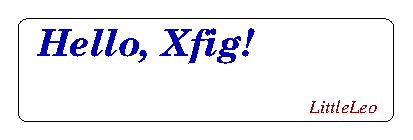
\includegraphics{hello}
  \caption{利用 Xfig 制图}
  \label{fig:xfig1}
\end{figure}

大学之道,在明明德,在亲民,在止于至善。知止而后有定;定而后能静;静而后能安;安
而后能虑;虑而后能得。物有本末,事有终始。知所先后,则近道矣。古之欲明明德于天
下者,先治其国;欲治其国者,先齐其家;欲齐其家者,先修其身;欲修其身者,先正其心;
欲正其心者,先诚其意;欲诚其意者,先致其知;致知在格物。物格而后知至;知至而后
意诚;意诚而后心正;心正而后身 修;身修而后家齐;家齐而后国治;国治而后天下
平。自天子以至于庶人,壹是皆以修身为本。其本乱而未治者 否矣。其所厚者薄,而其所
薄者厚,未之有也!

\hfill \pozhehao《大学》


\subsubsection{多个图形}
\label{sec:multifig}

如果多个图形相互独立,并不共用一个图形计数器,那么用 \verb|minipage| 或者
\verb|parbox| 就可以。否则,请参看图~\ref{fig:big1},它包含两个小图,分别是图~\ref{fig:subfig1} 
和图~\ref{fig:subfig2}。推荐使用 \verb|\subfloat|,不要再用
\verb|\subfigure| 和 \verb|\subtable|。
\begin{figure} %[h]
  \centering%
  \subfloat[第一个小图形]{%
    \label{fig:subfig1}
    
\includegraphics[height=2cm]{thu-fig-logo}}\hspace{4em}%
  \subfloat[第二个小图形。如果标题很长的话,它会自动换行,这个 caption 就是这样的例子]{%
    \label{fig:subfig2}
    
\includegraphics[height=2cm]{thu-text-logo}}
  \caption{包含子图形的大图形}
  \label{fig:big1}
\end{figure}

古之学者必有师。师者,所以传道受业解惑也。人非生而知之者,孰能无惑?惑而不从师,
其为惑也,终不解矣。生乎吾前,其闻道也固先乎吾,吾从而师之;生乎吾後,其闻道也亦
先乎吾,吾从而师之。吾师道也,夫庸知其年之先後生於吾乎!是故无贵无贱无长无少,道
之所存,师之所存也。

嗟乎!师道之不传也久矣,欲人之无惑也难矣。古之圣人,其出人也远矣,犹且从师而问焉;
今之众人,其下圣人也亦远矣,而耻学於师。是故圣益圣,愚益愚。圣人之所以为圣,愚
人之所以为愚,其皆出於此乎?爱其子,择师而教之,於其身也,则耻师焉,惑焉。彼童子
之师,授之书而习其句读者,非吾所谓传其道、解其惑者也。句读之不知,惑之不解,或师
焉,或不焉,小学而大遗,吾未见其明也。巫医、乐师、百工之人不耻相师,  士大夫之族
曰“师”曰“弟子”之云者,则群聚而笑之。问之,则曰:彼与彼年相若也,道相似也,位
卑则足羞,官盛则近谀。呜呼!师道之不复,可知矣。巫医、乐师、百工之人。吾子不齿,
今其智乃反不能及,其可怪也欤!圣人无常师。孔子师郯子、苌子、师襄、老聃。郯子之徒,
其贤不及孔子。孔子曰:“三人行,必有我师。”是故弟子不必不如师,师不必贤於弟子。
闻道有先後,术业有专攻,如是而已。

如果要把编号的两个图形并排,那么小页就非常有用了:
\begin{figure}
\begin{minipage}{0.48\textwidth}
  \centering
  
\includegraphics[height=2cm]{thu-whole-logo}
  \caption{并排第一个图}
  \label{fig:parallel1}
\end{minipage}\hfill
\begin{minipage}{0.48\textwidth}
  \centering
  
\includegraphics[height=2cm]{thu-whole-logo}
  \caption{并排第二个图}
  \label{fig:parallel2}
\end{minipage}
\end{figure}

李氏子蟠,年十七,好古文、六艺,经传皆通习之,不拘於时,学於余。余嘉其能行古
道,作师说以贻之。

\hfill \pozhehao 韩愈(唐)




%%% 其它部分
\backmatter

% 本科生要这几个索引,研究生不要。选择性留下。
\makeatletter
\ifthu@bachelor
  % 插图索引
  \listoffigures
  % 表格索引
  \listoftables
  % 公式索引
  \listofequations
\fi
\makeatother


% 参考文献
\bibliographystyle{thubib}
%\bibliography{ref/refs}
\bibliography{ref/Bibliography}


% 致谢

%%% Local Variables:
%%% mode: latex
%%% TeX-master: "../main"
%%% End:

\begin{ack}
  ���ĸ�л��ʦ xxx ���ں�����ϵ xxx �����ڶԱ��˵ľ���ָ�������ǵ��Դ����̽�ʹ
  ���������档

  ��������ʡ����ѧԺ��ѧϵ���оŸ��µĺ����о��ڼ䣬���� xxx ��������ָ�����������
  ʤ�м�����л xx ʵ�������� xx ���ڣ��Լ�ʵ����ȫ����ʦ��ͬѧ�ǵ����������֧
  �֣���������ɹ�����Ȼ��ѧ�����������ش���л��

  ��л \thuthesis�����Ĵ������ҵ�����д���������������࣬���ҵ����ĸ�ʽ����Ư����
  ���ࡣ

  ����ѧλ���ĵ���л��������ҳ��˶ʿ����ʿѧλ���IJ���ҳ�����Ա��ƿ��Զ�дһЩ��
  �о�����дһЩ��
\end{ack}


% 附录
\begin{appendix}
%%%% Local Variables: 
%%% mode: latex
%%% TeX-master: "../main"
%%% End: 

%\chapter{外文资料的原文}
%\label{cha:engorg}
%
%\section{Abstract}
%
%Research efforts on 3DTV technology have been strengthened worldwide recently, covering the whole media processing chain from capture to display. Different 3DTV systems rely on different 3-D scene representations that integrate various types of data. Efficient coding of these data is crucial for the success of 3DTV. Compression of pixel-type data including stereo video, multiview video, and associated depth or disparity maps extends available principles of classical video coding. Powerful algorithms and open international standards for multiview video coding and coding of video plus depth data are available and under development, which will provide the basis for introduction of various 3DTV systems and services in the near future. Compression of 3-D mesh models has also reached a high level of maturity. For static geometry, a variety of powerful algorithms are available to efficiently compress vertices and connectivity. Compression of dynamic 3-D geometry is currently a more active field of research. Temporal prediction is an important mechanism to remove redundancy from animated 3-D mesh sequences. Error resilience is important for transmission of data over error prone channels, and multiple description coding (MDC) is a suitable way to protect data. MDC of still images and 2-D video has already been widely studied, whereas multiview video and 3-D meshes have been addressed only recently. Intellectual property protection of 3-D data by watermarking is a pioneering research area as well. The 3-D watermarking methods in the literature are classified into three groups, considering the dimensions of the main components of scene representations and the resulting components after applying the algorithm. In general, 3DTV coding technology is maturating. Systems and services may enter the market in the near future. However, the research area is relatively young compared to coding of other types of media. Therefore, there is still a lot of room for improvement and new development of algorithms.
%
%\section{Introduction}
%
%Extending visual sensation to the third dimension has been investigated over decades. However, significant consumer mass markets haven't developed yet. 3-D video is established in niche markets, including professional applications (e.g., scientific visualization, medicine) and entertainment (IMAX cinemas, 3-D gaming). In recent years, research efforts have been strengthened worldwide to remove technological obstacles that encumber wider success of 3-D video applications \onlinecite{smolic20063d, onural2004overview, smolic20043dav, smolic2005interactive, onural2006assessment}. Significant improvements have been achieved for all components of the processing chain, from acquisition and signal processing, over 3-D scene representation, coding and transmission, to rendering and 3-D display. Very likely various 3-D video systems, components, applications and services will enter the market in the near future.
%
%Overviews of the state-of-the-art of technology for 3-D video are given in different papers of this Special Issue, each focusing on a specific component of the processing chain. This paper is devoted to coding. Various 3-D scene representation formats are used in different 3-D video systems and applications as de- scribed in \onlinecite{alatan2007scene}. These formats integrate various types of data, such as multiview video, and geometry data in form of depth or 3-D meshes. In general, 3-D video results in a tremendous amount of data that needs to be transmitted, stored or watermarked. Therefore, efficient compression is a key condition for the success of 3-D video. There is also a strong necessity for developing robust 3-D watermarking techniques, which protect the ownership rights. Further, the availability of open international standards is in general an important enabling factor for the development of markets in the media business. ISO/IEC JTC1/SC29/WG11 (Moving Picture Experts Group—MPEG) is one of the international standardization bodies that play an important role in digital media standardization. Therefore, this paper highlights MPEG standards for the different data as available and under development.
%
%The following section gives an overview of coding of multiview video, depth and associated data, with focus on avail- able and emerging MPEG standards. Section III is devoted to compression of static and dynamic 3-D mesh data as used for 3-D video representations as well as for 3-D computer graphics. Error resilience and multiple description coding (MDC) for 3-D is outlined in Section IV. Then, Section V elaborates on protection of 3-D content using watermarking. Finally, Section VI summarizes and concludes the paper.
%
%\section{Coding of Multiview Video, Depth, and Associated Data}
%
%Many 3DTV systems are based on scenarios, where a 3-D scene is captured by a number of cameras (see e.g., \onlinecite{tanimoto2004free, fujii2002free, matsuyama2004real, hamaguchi2003real, carranza2003free, wurmlin20033d, wurmlin20043d, matusik20043d}). The simplest case is classical stereo video with two videos. More advanced systems apply 8, 16, and more cameras. Some systems additionally apply per sample depth data that can also be treated as video signals. This section gives an overview of compression algorithms and standards for such data. An early overview of this research area can be found in \onlinecite{shum2003survey}. Depending on the degree of common content, shared by a subset of the cameras, a coding gain can be achieved in comparison to single-view coding. In multiview coding, correlations between adjacent cameras are exploited in addition to temporal correlations within each sequence. Therefore, multiview coding adds an- other compression dimension on top of single-view coding: the inter-view direction.
%
%\subsection{Conventional Stereo Video Coding}
%Stereo view is the most important special case of multiview with views. Compression of conventional stereo video has been studied for a long time and the corresponding standards are available. A conventional stereo pair consists of two images showing the same scene from two slightly different viewpoints corresponding to the distance of human eyes. The images are in general very similar, which makes them well suited for compression, e.g., with one image predicting the other. For instance one of them can be compressed without reference to the other stereo image. Then, the second image can be predicted from the already encoded one, just like temporally related images can be motion-compensated in video compression.
%
%The samples of both images correspond to each other through the 3-D geometry of the scene and camera properties, including positions and internal camera parameters such as the focal length. The displacement or disparity of each sample in one image with respect to the other is equivalent to a dense motion field in between two consecutive images of a video sequence. Therefore, it is justified to use the same principles of motion estimation and motion compensation for disparity estimation and disparity compensation for image prediction and then to only encode the prediction error or residual further.
%
%Nevertheless, some specific differences between motion compensation and disparity compensation need to be considered. The statistics of disparity vector fields is different from the statistics of motion vector fields. Disparities are biased and relatively large. Zero disparity means a very large depth of the corresponding point in 3D, while 3-D points close to the camera may have very large disparity values. This may require adjustments of entropy coding of the disparity vectors. In general temporally adjacent images of a video sequence tend to be more similar than views of a stereo pair at practical frame rates. Disocclusion effects, i.e., content that is visible in one image is occluded in the other and can therefore not be predicted, are on average more evident in a stereo pair than in between two temporally adjacent video images. Further, specific differences in a stereo pair may come from incorrect white and colour balance but also due to scene lighting and surface reflectance effects.
%
%\begin{figure}[htbp]
%\begin{center}
%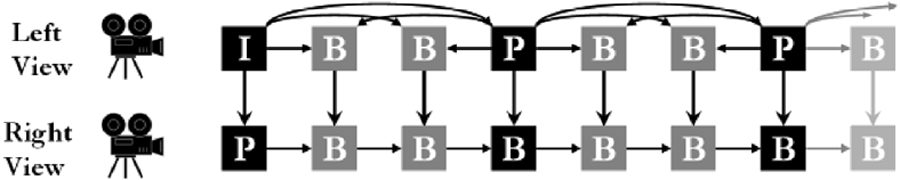
\includegraphics[width=0.8\textwidth]{predh262.png}
%\caption{Illustration of prediction in H.262/MPEG-2 Video multiview profile}
%\label{fig:predh262}
%\end{center}
%\end{figure}
%
%
%The combination of inter-view and temporal prediction is the basic principle for efficient compression of conventional stereo video. A corresponding standard specification has already been defined in ITU-T Rec. H.262/ISO/IEC 13818-2 MPEG-2 Video, the Multiview Profile \onlinecite{haskell1997digital, itu1994mpeg2}, as illustrated in Fig. \ref{fig:predh262}. The left eye view is encoded without reference to the right eye view, using standard MPEG-2. This ensures backward compatibility with Main Profile of H.262/MPEG-2 Video, since it is possible to decode the left eye view bit stream and to display 2-D video. For the right eye view, inter-view prediction is allowed in addition to temporal prediction.
%
%However, the gain in compression efficiency compared to independent encoding of both video streams is rather limited. This is mainly due to the fact that temporal prediction already provides very good performance. Typically, if temporal prediction is efficient for a certain image (e.g., B-pictures for right view in Fig. \ref{fig:predh262}) then additional inter-view prediction does not increase the coding performance significantly. Temporal neighbouring images are typically on average more similar than spatially neighbouring images.
%
%For images that are coded as I-pictures, i.e., without reference to other temporally adjacent images in the video sequence, a significant gain can be achieved by inter-view prediction. Typically every 0.5–1 s such I-pictures are inserted into a video stream to enable random access and error robustness. In Fig. \ref{fig:predh262}, the left-hand side picture of the left view is encoded as I-picture. The corresponding left-hand side picture of the right view would also be encoded as I-picture for random access when in- dependently encoding both video streams. However, in H.262/ MPEG-2 Video multiview coding, inter-view prediction can be applied, resulting in a significant increase of compression efficiency compared to coding this picture as I-picture.
%
%Research on compression of conventional stereo video has continued into several directions, including for instance optimum joined bit allocation for both channels, or abandoning backward compatibility to design more efficient inter-view prediction structures. Algorithms have been based on more up-to-date video codecs such as H.263\onlinecite{itu1995h263}, MPEG-4 Visual\onlinecite{itu1999mpeg4}, or H.264/AVC\onlinecite{sun2005stereo, wiegand2003overview, itu2003h264}. However, none of the developments including the original Multiview profile have reached commercial relevance so far, since the application of stereo video did not develop into a relevant mass market yet.
%
%\subsection{Compression of Video Plus Depth Data}
%
%An alternative to classical stereo video as described in the previous section is to transmit a video signal and a per sample depth map. From the video and depth information, a stereo pair can be rendered at the decoder \onlinecite{fehn2002evolutionary, fehn20043d}. This extends the functionality since it enables head motion parallax viewing if the user’s head motion is tracked. Additionally, this format is interesting from compression efficiency point of view. Per sample depth data can be regarded as a monochromatic, luminance-only video signal. The depth is restricted to a range between two extremes $Z_{near}$ and $Z_{far}$ indicating the minimum and maximum distance of the corresponding 3-D point from the camera respectively. The depth range is linearly quantized with 8 bit, i.e., the closest point is associated with the value 255 and the most distant point is associated with the value 0. With that, the depth map is specified, resulting in a grey scale image. These grey scale images can be fed into the luminance channel of a video signal and the chrominance can be set to a constant value. The resulting standard video signal can then be processed by any state-of-the-art video codec.
%
%Results from the European ATTEST project \onlinecite{fehn2002evolutionary} have shown that depth data can be very efficiently compressed this way. Several state-of-the-art video codecs have been tested (MPEG-2, MPEG-4, H.264/AVC). A course estimate indicates that 10\%–20\% of the bit rate which is necessary to encode the colour video is sufficient to encode the depth at good quality. This is due to the specific statistics of depth data, being on average smoother and less structured that colour data.
%
%Based on these observations, a new backward compatible (with respect to classical DVB) approach for 3DTV was developed in the ATTEST project. It uses a layered bit stream syntax. The base layer is a conventional 2-D colour video encoded using MPEG-2. This base layer can be processed by any existing MPEG-2 decoder providing backward compatibility. Additionally the bit stream contains an advanced layer carrying the encoded depth information. Advanced systems may access this layer to decode the depth stream and then generate a stereo pair to be displayed stereoscopically by view interpolation.
%
%This concept is highly interesting due to the backward compatibility, compression efficiency and extended functionality compared to conventional stereo video. Moreover, it does not introduce any specific coding algorithms. It is only necessary to specify high-level syntax that allows a decoder to interpret 2 incoming video streams correctly as colour and depth. Additionally information about depth range($Z_{near}$ and $Z_{far}$) needs to be transmitted. Therefore, MPEG specified a corresponding container format “ISO/IEC 23002-3 Representation of Auxiliary Video and Supplemental Information,” also known as MPEG-3 Part 3, for video plus depth data \onlinecite{iso2007rep, iso2007fdam}. Moreover, H.264/AVC contains an option to convey the depth images through its auxiliary picture syntax. Here, the video codec for the colour video signal and associated depth video signal are both H.264/AVC. This approach is backwards compatible with any existing deployment of H.264/AVC.
%
%A general problem of the video plus depth format is content creation, i.e., the generation of depth information. Cameras that automatically capture per pixel depth with the video are available and are being further enhanced, but the quality of the captured depth fields is currently still limited. Algorithms for depth estimation have been studied extensively in computer vision literature and powerful solutions are available. However, it always remains an estimation that can only be solved up to a residual error probability. Estimation errors influence the quality of rendered views. A fully automatic, accurate and reliable depth capturing system is still to be developed. User-assisted content generation is an option for specific applications. Even having perfect depth available, artifacts may occur in rendered views due to disocclusion. This effect increases with the distance of the virtual view from the original camera position. Additional occlusion layers (layered depth video as extension of layered depth images \onlinecite{shade1998layered}) or extension to multiview video plus depth \onlinecite{zitnick2004high, kauff2007depth}, help to minimize these problems at the cost of increased data rate and complexity.
%
%\subsection{Multiview Video Coding}
%
%\begin{figure}[htbp]
%\begin{center}
%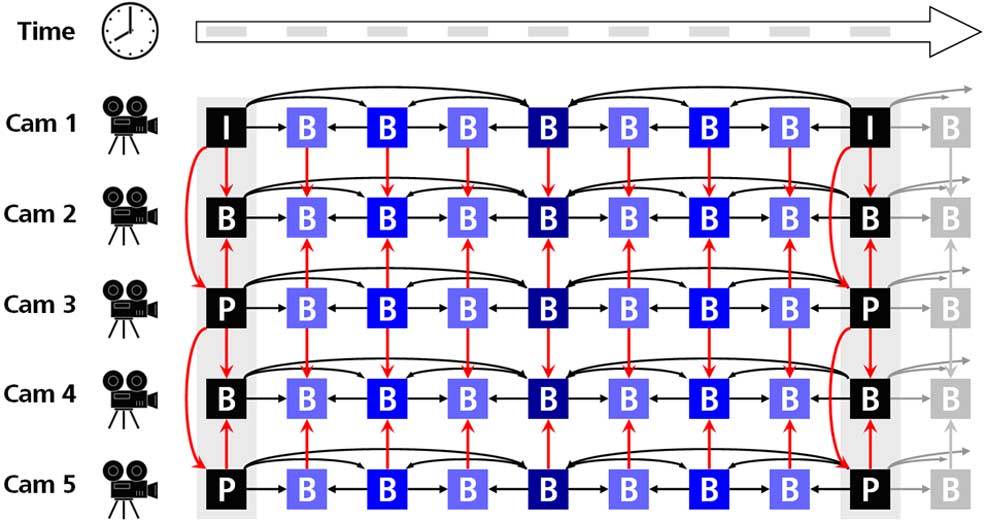
\includegraphics[width=0.8\textwidth]{tempinterpred.jpg}
%\caption{Temporal/inter-view prediction structure for MVC.}
%\label{fig:tempinterpred}
%\end{center}
%\end{figure}
%
%A common element of many 3DTV systems is the use of multiple views of the same scene that have to be transmitted to the user. The straight-forward solution for this would be to encode all video signals independently using a state-of-the-art video codec such as H.264/AVC. However, multiview video contains a large amount of inter-view statistical dependencies, since all cameras capture the same scene from different view-points. These can be exploited for combined temporal/inter-view prediction, as illustrated in Fig. \ref{fig:tempinterpred}. Images are not only predicted from temporally neighbouring images but also from corresponding images in adjacent views. Statistical evaluations have shown that significant gain can be expected from such combined temporal/inter-view prediction \onlinecite{merkle2005statistical, kaup2006analysis}. Pioneering work on multiview image coding is reported in \onlinecite{magnor2000data, magnor2003multi}.
%
%Several research groups addressed multiview video coding (MVC) and developed dedicated inter-view/temporal prediction structures to efficiently exploit all statistical dependencies within the multiview video data sets (see e.g., \onlinecite{oh12542multi, cheng2006multi, yang2006hyper, vetro2004coding, kalva2006design, socek2006permutation, kalva2006challenges, bilen2006multi}. Among those, algorithms that are based on hierarchical B-pictures \onlinecite{schwarz2006analysis} as supported by H.264/AVC syntax in temporal and inter-view dimension (Fig. \ref{fig:tempinterpred}) proved best performance in exhaustive experiments conducted in the context of MPEG standardization \onlinecite{flierl2007motion, merkle2006efficient, mueller2006multi, merkle2007efficient}. In these experiments, it has been shown by objective and subjective measurements that dedicated MVC outperforms independent encoding of the multiple video streams significantly. However, the achievable gain strongly depends on the content and its properties such as camera distance, frame rate and complexity of the content (motion, texture). For some data sets the peak signal-to-noise ratio (PSNR )gain was reported as 0.5 dB and below. Maximum reported gains were up to 3dB.
%
%A drawback of combined temporal/inter-view prediction as illustrated in Fig. \ref{fig:tempinterpred} is the complexity. This includes computational complexity, memory requirements and delay. In \onlinecite{merkle2007efficient, merkle2007coding}, it has been shown that the complexity can be significantly decreased without sacrificing much coding efficiency. Inter-view prediction is restricted here to the key pictures that would be treated as I-pictures in independent encoding of the views (e.g., time and in Fig. \ref{fig:tempinterpred}). Most of the coding gain of MVC comes from inter-view prediction of these pictures that do not use temporal prediction for temporal random access reasons. Omitting inter-view prediction for pictures that have a temporal reference does not cost much coding efficiency whereas it decreases complexity significantly.
%
%In addition to combined temporal/inter-view prediction, specific MVC algorithms have been proposed. The basic idea of depth/disparity-based view interpolation prediction \onlinecite{martinian2006view, kitahara2006multi, martinian2006extensions} is to estimate depth or disparity either at the encoder (this requires overhead for sending the depth/disparity) or the decoder, and to perform view interpolation or 3-D warping for prediction. However, the gains reported so far are marginal. Only for very few test data sets with very close camera settings such view interpolation prediction provides a gain of up to 5\% bit rate saving at the same visual quality. Further investigations are needed to optimize the performance.
%
%Further, illumination and color inconsistencies affect the exploitation of inter-view statistical dependencies. Usually such effects should be minimized by proper setting of the conditions, however, an MVC algorithm should also be able to cope with this as well, since proper white and color balancing of the input can not be guaranteed. Also, the illumination (spotlights, shadows, etc.) varies largely over the multiview images due to the lighting conditions. These problems might be handled by proper illumination and color compensation as proposed in \onlinecite{kim2006results} and \onlinecite{lee2006results}. The basic idea is to modify the motion compensation on macroblock level. Before subtracting the pixel values of the block to be encoded and the reference block, the mean of each is compensated from the corresponding pixel values. This assumes locally constant illumination and color variations, which is an appropriate model trading-off accuracy and complexity. Gains of up to 0.7 dB have been reported for some test data using illumination compensation. However, this strongly depends on the test data and in some cases the gain is negligible or there is none at all. On average over all test data sets a bit rate reduction of 5\% was reported for the same visual quality.
%
%An alternative to illumination compensation on macroblock level integrated into the encoding process, also an appropriate preprocessing can be applied, prior to encoding. Algorithms for illumination correction are well-known in image and video processing. Then the corrected data can be passed to a standard encoder. The big advantage of such an approach is that no changes are necessary to the encoder, decoder and bit stream syntax. A preliminary investigation in this direction is presented in \onlinecite{fecker2006improving}, however, results are not complete and performance in comparison to integrated illumination compensation is not clear.
%
%Another research direction is improving disparity estimation, compensation, and coding \onlinecite{lu2009effective}. Mostly disparity is treated equally to motion, however, it is known that the statistical properties of disparity vectors can be quite different compared to those of motion vectors. Disparity estimation has been studied extensively in the computer vision literature. Usually, basic geometric properties and constraints are taken into account. For instance, the search can be done along epipolar lines.
%
%This may lead to better estimates and reduce the complexity. Further, specific disparity coding may improve the efficiency of inter-view prediction. Specific coding modes for MVC such as the inter-view direct mode \onlinecite{guo2006inter} are under investigation.
%
%Combination of scalability with MVC is investigated for in- stance in \onlinecite{garbas20064d, drose2006extending, yang20064, yang2005scalable, ozbek2006scalable}. So far the feature of scalability only comes with decreased compression efficiency. Distributed MVC is investigated for instance in \onlinecite{guo2006distributed}. Also first work on efficient trans- port and delivery taking user interactivity into account has been presented \onlinecite{kurutepe-interactive, kurutepe2006interactive}. Finally, efficient mechanisms for optimum random access, parallel processing and memory management for MVC have been investigated.
%
%Since the results clearly indicate that MVC outperforms independent encoding of the multiple video signals, and there is a clear demand from industry for a corresponding standard, ISO/ MPEG and ITU/VCEG decided developing a dedicated MVC specification \onlinecite{vetro-joint, vetro2006joint}. It will be an extension of H.264/AVC (Amendment 4), which is scheduled to be finalized in 2008. MVC is the main focus of this Special Issue. We therefore refer the reader to the dedicated articles in this volume that contain all details of state-of-the-art MVC technology.
%
%\subsection{Conclusions and Future Research Directions}
%
%Research on coding of stereo video, multiview video and associated depth or disparity data has reached a good level of maturity. Related international standards are available enabling a variety of 3DTV systems and applications. However, compared to coding of other types of media data the scientific field is relatively young, and therefore there is still a lot of room for improvement of algorithms. This includes for instance optimization of MVC and development of new specific coding MVC algorithms. Depth or disparity coding may be improved further by development of dedicated algorithms. Further, there are more complex types of data representations for 3DTV such as layered depth video and multiview video plus depth that provide extended functionality. Efficient coding algorithms for such data are still under investigation. Initial results are reported in \onlinecite{merkle2007efficientmvc} and \onlinecite{merkle2007multi}. Other types of multiview representations are also under investigation often related to specific types of 3-D displays. An example is presented in \onlinecite{saishu2006flatbed}.
%
%%\cleardoublepage

\chapter{外文资料的书面翻译}

\section{摘要}

最近,3D电视技术相关的研究工作在全球范围内都有增加。这些研究覆盖了整个媒体处理流程,从采集到显示无所不包。不同的3D电视系统依靠各种类型数据构成的不同的3D场景表示方式。对这些数据的高效编码对于3D电视的成功至关重要。对双目视频、多视点视频、深度图或视差图中像素类型数据的压缩拓展了已有的经典视频编码的原则。针对多视点视频和视频加深度数据的强大算法和开放的国际标准已经出现并一直有着进展,这为在不久的将来引进各种3D电视系统奠定了基础。对3D网格模型的压缩也达到了高度成熟的程度。对静态的几何体,有多种强大的算法可以有效地压缩顶点和连接数据量。对动态3D几何体的压缩是现在更受关注的研究方向。基于时间的预测是一个重要的对动画3D网格序列去冗余信息的机制。容错性对于在易出错的信道上传输数据十分重要,而多描述编码(MDC)是一种可行的保护数据的方法。对静态图和2D视频的MDC已经得到了广泛的研究,但是对多视点视频和3D网格的MDC最近才刚刚提出。用水印进行3D数据的知识产权保护也是一个前沿的研究方向。3D水印方法方面的文献根据表示场景的主要部分在应用算法前后的维数可以归为三类。总而言之,3D电视编码技术正在走向成熟。相关系统和服务可能在不久的将来进入市场。然而,这个方向的研究相对其他媒体数据的研究而言又很少,所以仍有很大的空间可以改进,有很多新的算法可能被提出。

\section{简介}

将我们的视觉延伸到三维空间在近几十年中一直都在研究,但是大规模的消费市场仍然没有发展起来。3D视频还在小众市场发展,包括专业应用(比如科学数据可视化、医药学等)和娱乐方面(比如IMAX影院、3D游戏等)。近年来,更多的研究精力投向了这个领域,以期能够跨越阻碍3D视频应用得到更广泛成功应用的障碍\cite{smolic20063d, onural2004overview, smolic20043dav, smolic2005interactive, onural2006assessment}。从获得信号、处理信号到3D场景表示、编码、传输,再到渲染和3D显示,整个处理流水线的各个部分都取得了显著的进步。很可能在不久的将来,各种3D视频系统、组件、应用和服务就会进入市场。

这一期中给出了各种尖端3D视频技术的综述,分别针对一个3D视频处理流水线中的一个特定组件。这篇文章介绍编码相关的部分。\onlinecite{alatan2007scene}中介绍了用在不同的3D视频系统和应用中的不同3D场景表示格式在。这些格式整合了各种类型的数据,比如多视点视频、深度或3D网格的几何数据。总的来说,3D视频就意味着有大量的数据需要传输、存储和水印。于是高效的压缩就是3D视频成功与否的一个关键条件。同时对发明一个鲁棒的3D水印技术来保护所有权也有很强的需求。此外,开放的国际标准对市场和相关商业的发展也是一个推动力。ISO/IEC JTC1/SC29/WG11 (Moving Picture Experts Group—MPEG)就是一个在数字媒体标准化中起到重要作用的国际标准化组织。所以,这篇文章关注现有的和正在成形的各种数据的MPEG标准。

接下来的几节分别给出多视点视频、深度和关联数据的编码综述,集中关注已有的和正在成形的MPEG标准。第3节介绍用于3D视频表示以及3D计算机图形学的静态和动态3D网格数据的压缩。容错以及3D视频的多描述编码(MDC)在第4节中介绍。然后在第5节中介绍用水印保护3D内容的方法。最后,第6节概况和总结这篇文章的观点。

\section{多视点视频、深度和关联数据编码}

很多3D电视系统都基于场景,这些3D场景由N个相机获取(见\onlinecite{tanimoto2004free, fujii2002free, matsuyama2004real, hamaguchi2003real, carranza2003free, wurmlin20033d, wurmlin20043d, matusik20043d})。最简单的情形就是经典的两路视频构成的立体视频,更复杂一些的系统用8路、16路或更多路相机获取的视频。有些系统还使用可以当作视频信号的深度信息。这一节综述这类数据的压缩算法和标准。更早对这个研究方向的综述可以参见\onlinecite{shum2003survey}。通过共享内容、共享一些相机,多视点视频比起单视点视频的编码可以一定提升。在多视点视频编码中,除了挖掘单个相机的数据在时间上的关联之外,临近的相机之间的关系也被挖掘出来。于是多视点视频在单视点视频的基础上增加了一个新的压缩维度:视点间的方向。

\subsection{传统立体视频编码}

立体视频是多视点视频中最重要的一个特例,是有N=2个视点的情形。 压缩传统的立体视频已经经过了长时间的研究,相关的标准也已经问世。一个传统的立体对由从两个略微不同的视点(对应人的瞳距)观察同一场景的两幅静态图组成。这两幅图片总的来说极其相似,使得它们很适合压缩,比如从一幅图片预测另一幅。例如,其中一幅可以不参考另一幅而单独压缩,而第二幅图片可以从已经编码的一幅图片来预测,就像视频压缩中的基于时间预测的动态补偿那样。
 
对两幅图片的样本基于场景和相机属性(包括位置和相机内部参数比如焦距)的3D几何各自对应起来。每个样本的位移或视差就等价于一个视频序列中两幅连续图像的dense motion field。于是就可以用运动估计和运动补偿一样的方法去做视差分析和视差补偿,以此实现图像预测,然后就只需要编码预测误差或者进一步的残差即可。

然而,一些特定的动态补偿和视差补偿间的区别需要考虑进来。视差向量场的统计与运动向量场的统计不同。视差是有偏的,而且相对较大。零视差以为着一个点在 3D场景中的深度极大,而一个距离相近很近的3D点会有很大的视差值。这需要对视差向量的熵编码做调整。总的来说,在正常的帧率下,视频序列中在时间上邻近的图像倾向于比立体视频的两个视点的图像更加相似。图像损失(内容在一张图中可见但是在另一张图中不存在,也就无法被预测)平均来说在立体视频中出现得比时间上邻近的两幅图更多。此外,立体图片对中的差别可能来自不正确的白平衡或色彩平衡,也可能来自场景的光照和表面反射效果的差别。 

\begin{figure}[htbp]
\begin{center}
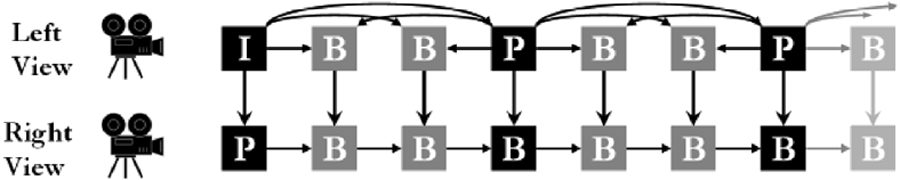
\includegraphics[width=0.8\textwidth]{predh262.png}
\caption{H.262/MPEG-2视频多视点类(multiview profile)的预测示意}
\label{fig:predh262chs}
\end{center}
\end{figure}

视角间和时间上的预测组合是有效压缩传统立体视频的基本方法。对应的标准已经在ITU-T Rec.H.262/ISO/IEC 13818-2 MPEG-2Video, the Multiview Profile\cite{haskell1997digital, itu1994mpeg2}中定义了,如图\ref{fig:predh262chs}所示。左眼视频不参考右眼视频单独编码,使用标准的MPEG-2。这保证了对H.262/MPEG-2的主类(Main Profile)的前向兼容性,因为这样可以解码左眼视频流来显示2D视频。对右眼视频,时间轴预测之外还可以允许做视点间预测。
 
然而,对比分别压缩两个视频流而言,这样的压缩效率提升很有限。这主要是由于基于时间的预测已经达到了很高的性能。特别是当基于时间的预测对于一张特定图像效率不错的时候(比如图\ref{fig:predh262chs}中右眼视频的B帧),那么增加视角间的预测就无法显著提升编码性能了。时间上邻近的图像平均而言一般都比空间上邻近的图像更相似。

对于编码为I帧的图像,也就是说不参考其他视频序列中时间上邻近的帧来编码的帧,加入视角间的预测有明显成效。一般每半秒到一秒时间就会在视频序列中插入这样一个I帧来保证随机访问和容错性。在图\ref{fig:predh262chs}中,左眼序列的最左侧一帧被编码为I帧,当分别编码两个视频序列时,对应的右眼序列中的那一帧也可以编码为I帧。但是在H.262/MPEG-2视频多视点编码中,可以采用视角间预测来达到压缩效率上比编为I帧方式的显著提升。

对于传统立体视频压缩的研究还在各个方向上继续进行着,包括对各个频道的最优码率分配以及放弃前向兼容去设计一个更加有效的视角间预测的结构。相关算法是都是基于更新的视频编码比如H.263\cite{itu1995h263},MPEG-4 Visual\cite{itu1999mpeg4}或H.264/AVC \cite{sun2005stereo, wiegand2003overview, itu2003h264}。但是由于立体视频的应用还没有发展到一个足够大的市场,所有这些进展包括原有的多视点类(Multiview profile)都尚未能商业化。

\subsection{视频加深度数据的压缩}

除了前文描述的经典立体视频外,还有一种传输视频信号的方式——传输一路视频和每个样本的深度图。从视频和深度信息,可以在解码端渲染出一对立体图\cite{fehn2002evolutionary,fehn20043d}。这提供了另一项功能:当用户的头部移动被捕捉到时,能够提供相对应的观察角度的图像。此外,这种格式从压缩效率的角度来看很有价值。深度信息可以被当作单色、仅有明度的视频信号。深度被限制在两个表示对应3D点到摄像机的最小和最大距离的极限距离$Z_{near}$和$Z_{far}$之间。深度范围线性地量子化到8位,也就是最近的点赋值255,最远点赋值为0。这样一来,一张深度图就确定下来了,成为一张灰度图。这些灰阶图可以被插入视频信号的光照信道中,其色彩可以被设定为一个常数。这样获得的标准视频信号就可以用任何先进的视频编码处理了。

欧洲ATTEST的一个项目\cite{fehn2002evolutionary}结果表明深度信息可以用这种方式非常高效地压缩。一些前沿的视频编码参与了测试(MPEG-2, MPEG-4, H.264/AVC)。一项估计显示,只要编码彩色视频信号10\%到20\%的比特率就足以编码高质量的深度信息了。

基于这些观察,这个ATTEST项目提出了一种新的(对比经典的DVB)向前兼容的实现3DTV的方式。它采用一种分层的比特流语法。基层是一个传统的 MPEG-2编码的彩色2D视频。基层可以被任何现有的MPEG-2解码器处理,保证前向兼容性。除此之外,比特流还包含更高一层传输编码后的深度信息。更高级的系统可以访问这一层来解码深度信息,然后通过插值生成一对立体图像来显示。

这种概念由于保证了前向兼容性、压缩率高并且相比传统立体视频功能扩展更多,所以非常有价值。不仅如此,它并不引入一种特定的编码算法。只需要制定一种高层的语法,让解码器能够把输入的两路视频正确地分辨成一路视频和一路深度即可。附加的深度信息($Z_{near}$和$Z_{far}$)需要另外传输。所以MPEG为视频加深度信息制定了一种对应的容器格式 “ISO/IEC 23002-3 Representation of Auxiliary Video and Supplemental Information”,或者称为MPEG-3 Part 3\cite{iso2007rep, iso2007fdam}。此外,H.264/AVC包含一个选项通过辅助的图片语法传输深度图。此处对彩色视频信号和对应的深度视频信号的视频编码都用的是 H.264/AVC。这种方法对任何已部署的H.264/AVC设备都能做到前向兼容。

对视频加深度的格式而言,有一个普遍存在的问题就是深度信息的生成。能够在捕获视频的同时自动获取每个像素深度的摄像机已经问世而且在进一步增强,但是得到的深度场的精度还是很有限。计算机视觉相关的文献中对深度估计的算法有了很深入的研究,强大的解决方案也已经出现。但是这总是一个建立在一定残差误差概率上的估计值。估计的误差会影响渲染出的图像的质量。全自动而且精确的深度获取系统仍然有待开发。对于特定的应用,用户辅助的内容生成可以作为一种选择。即使有了完美的深度图,遮挡也会使渲染出的图像有瑕疵。这些效应在距离原始摄像机位更远的虚拟点上会更加严重。增加一些层(深度视频层作为深度图像层的扩展\cite{shade1998layered})或者扩展到多视点视频加深度\cite{zitnick2004high, kauff2007depth}能够以增加数据量和复杂度为代价,帮助减小这些问题。

\subsection{多视点视频编码}

\begin{figure}[htbp]
\begin{center}
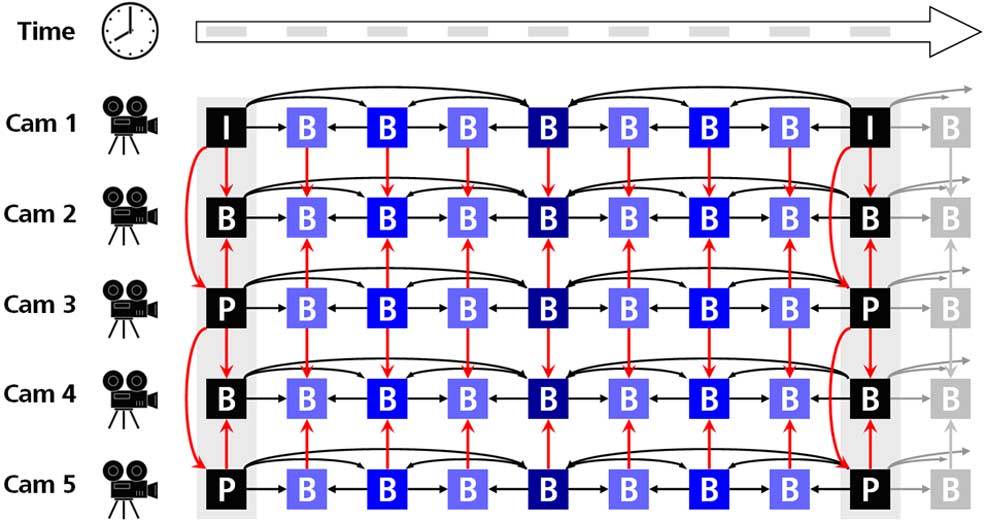
\includegraphics[width=0.8\textwidth]{tempinterpred.jpg}
\caption{MVC的时间和视角间预测结构}
\label{fig:tempinterpredchs}
\end{center}
\end{figure}

3DTV系统的一个共同部分是传输给用户的同一场景不同视角视频的使用。最直接的解决方法就是把所有的视频信号分别用最新的编码方式比如 H.264/AVC编码。但是多视点视频在视角间存在统计意义上很大的相关性,因为每个摄像机捕获的都是不同视角的同一场景的图像。这些相关性可以用来进行时间和视角间预测,如图\ref{fig:tempinterpredchs}所示。图像不仅仅根据时间上临近的图来预测,还根据相邻视角的对应图像预测。统计表明这样的组合式预测能够极大地提高编码效率\cite{merkle2005statistical, kaup2006analysis}。多视点图像编码的前沿研究在\onlinecite{magnor2000data, magnor2003multi}中有报告。

几个研究小组提出了多视点视频(MVC),并且发展了专门的视角间和时间预测的架构来有效地挖掘利用多视点视频数据集中的统计相关性(见\onlinecite{oh12542multi, cheng2006multi, yang2006hyper, vetro2004coding, kalva2006design, socek2006permutation, kalva2006challenges, bilen2006multi})。其中,H.264/AVC时间和视角间预测的语法支持的基于B帧的算法\cite{schwarz2006analysis}在MPEG标准的穷尽测试下被证明是性能最好的\cite{flierl2007motion, merkle2006efficient, mueller2006multi, merkle2007efficient}。在这些实验中,客观和主观的测量都显示MVC极大地超越了独立压缩各个视频。然而,能够获得的提升极其依赖内容和相机间距、帧率、内容复杂度(运动、纹理)等属性。对于一些数据集,信噪比峰值(PSNR)增益在0.5dB以下。最大的增益达到过3dB。

图\ref{fig:tempinterpredchs}中描述的时间和视角间组合预测的一个不足就是其复杂度。包括计算复杂度、内存需求和延迟。在\onlinecite{merkle2007efficient, merkle2007coding}中提到,复杂度在不牺牲多少编码效率的情形下可以极大地降低。视角间预测此时被限制在作为I帧独立编码的关键帧上(例如图\ref{fig:tempinterpredchs}中的$t_0$和$t_8$)。MVC中大部分编码增益来自于这些为了随机访问而不进行视角间预测的帧。忽略有时间预测的帧的视角间预测并不消耗多少编码效率却显著降低复杂度。

在结合时间和视角间预测之外,专门的MVC算法被提了出来。基于深度/视差的视角间插值预测\cite{martinian2006view, kitahara2006multi, martinian2006extensions}的基本思想是在编码(这需要另外传输深度/视差)或解码端估计深度或视差,然后进行视角间插值或者3D扭曲来预测。但是目前得到的增益不高。仅仅对于摄像机参数极其接近的很小一部分数据集,这样的视角间插值预测在同样画质下能节省5\%的比特率。想要优化性能还要做进一步的研究。

不仅如此,光照和色彩的不一致影响了对视角间统计相关性的挖掘。通常这样的效应能被正确的条件设定减小,但是 MVC算法也要能够应对这样的情形,因为输入的白平衡和色彩平衡并不能保证。同样,一定的光照条件下,光照(聚光灯、阴影等)在视角间会有很大的不同。这些问题或许能通过\onlinecite{kim2006results}和\onlinecite{lee2006results}中提出的正确的光照和色彩补偿来解决。基本思想是在宏块级别修改运动补偿。在对待编码帧块和参考块的像素值相减之前,二者的平均值根据对应的像素值做补偿。其中假设了本地的光照和色彩变化是常值,这是个模型的准确率和复杂度之间的权衡。对于一些测试数据,光照补偿获得了0.7dB的增益。但是这个增益极大地依靠测试数据,在一些情况下,增益可以忽略甚至根本不存在。对所有的测试数据集平均下来,相同视觉质量下,能够节省5\%的比特率。

另一种宏块级别的光照补偿可以整合到编码过程中,一个合适的预处理也可以在编码前进行。对图像和视频的光照更正算法广为人知。然后更正过的数据可以被传到一个标准的编码器。这种方法的一大优势是编码器、解码器和码流语法不需要做任何改动。一项这个方向上的前期调研发表在\onlinecite{fecker2006improving}中,但是结果并不完全,性能与整合光照补偿的比较也不清楚。

另一个研究方向是改进视差估计、补偿和编码\cite{lu2009effective}。多数的视差都被当作运动来对待,但是我们知道视差向量的统计属性和运动向量可以完全不同。视差估计在计算机视觉文献中已经被广泛研究。通常,级别的几何属性和约束会考虑进来。比如搜索可以通过沿着核极线(epipolar lines)完成。这可能带来更好的估计和降低复杂度。此外,专门的视差编码或许能提高视角间预测的编码效率。专门的MVC编码模式比如视角间直接模式\cite{guo2006inter}正在研究中。

MVC的扩展性结合正在被研究,比如\onlinecite{garbas20064d, drose2006extending, yang20064, yang2005scalable, ozbek2006scalable}。目前可扩展的功能仅能依靠降低压缩效率。分布式MVC在\onlinecite{guo2006distributed}中被研究。加入用户交互考虑的有效传输在\onlinecite{kurutepe-interactive, kurutepe2006interactive}中初次被讨论。最后,能够随机访问的有效的MVC编码机制、并行处理和内存管理也正在研究中。

由于结果明显表明MVC优于单独编码各路视频信号,业界又显然需要一个对应的标准,ISO/MPEG和ITU/VCEG 决定发展一种专门的MVC标准\cite{vetro-joint, vetro2006joint}。这会是一个H.264/AVC的扩展(第4修正案),这预计在2008年内完工。MVC是这一期特刊的主要关注点。我们因此向读者介绍包含最前沿MVC技术的文章。

\subsection{结论和未来研究方向}

对立体视频、多视点视频和相关深度、视差数据的研究已经有很高的成熟度。相关的国际标准也已经问世,使3DTV系统和应用成为可能。然而,相对于其他类型和媒体数据的编码,这个领域还很年轻,算法还有很大的进步空间。这包括对MVC实力的优化和新的专门的MVC算法的开发。深度和视差编码可能在将来的专门的算法中进一步优化。此外,有更多复杂的3DTV数据结构比如分层的深度视频和多视点视频加深度来提供更多的功能。对这些数据的有效编码算法还在研究之中。初步的结果在\onlinecite{merkle2007efficientmvc}和\onlinecite{merkle2007multi}中有报告。其他多视点描述的类型也在研究中,这往往和特定的一类3D显示器相关。\onlinecite{saishu2006flatbed}中有一个例子。

\begin{center}
\heiti{原文索引}
\end{center}

Smolic A, M{\"u}eller K, Stefanoski N, et al. Coding algorithms for 3DTV—a survey. IEEE transactions on circuits and systems for video technology, 2007, 17(11):1606–1620

%\cleardoublepage

%%% Local Variables: 
%%% mode: latex
%%% TeX-master: t
%%% End: 

\chapter{实验数据表格}
\label{cha:expdatatable}

\begin{longtable}[\textwidth]{lrrr}
\caption{VS2008性能分析报告(前50项记录)}\label{tab:vs50}\\
\toprule[1.5pt]
\multicolumn{1}{l}{\textbf{Function Name}} & \multicolumn{1}{r}{\textbf{Exclusive Time}} & \multicolumn{1}{r}{\textbf{Exclusive Time \%}} & \multicolumn{1}{r}{\textbf{Number of Calls}}\\
\midrule[1.5pt]
\endfirsthead
\multicolumn{4}{c}{续表~\thetable\hskip1em VS2008性能分析报告(前50项记录)}\\
\toprule[1.5pt]
\multicolumn{1}{l}{\textbf{Function Name}} & \multicolumn{1}{r}{\textbf{Exclusive Time}} & \multicolumn{1}{r}{\textbf{Exclusive Time \%}} & \multicolumn{1}{r}{\textbf{Number of Calls}}\\ 
\midrule[1pt]
\endhead
\hline
\multicolumn{4}{r}{续下页}
\endfoot
\endlastfoot
\rowcolor{gray!15}
    macroblockPredGetDataUV		&	341.01	&	14.41	&	2,632,478	\\
    macroblockPredGetDataY		&	321.37	&	13.58	&	1,316,239	\\ \rowcolor{gray!15}
    idct4x4\_c						&	316.86	&	13.39	&	5,028,960	\\
    macroblockGetPred\_axb		&	181.29	&	7.66 	&	1,316,239	\\ \rowcolor{gray!15}
    macroblockGetPred\_axb\_Bi	&	133.42	&	5.64 	&	571,944		\\
    macroblockGetHalfPel			&	132.47	&	5.6  	&	148,552		\\ \rowcolor{gray!15}
    Filter							&	101.92	&	4.31 	&	6,215,308	\\
    addMacroblockdata				&	85.36	&	3.61 	&	184,171		\\ \rowcolor{gray!15}
    iquant4x4\_c					&	84.48	&	3.57 	&	5,028,960	\\
    macroblockPBPrediction		&	70.95	&	3    	&	184,171		\\ \rowcolor{gray!15}
    macroblockInterDecode\_uv		&	67.05	&	2.83 	&	184,171		\\
    save\_data\_pb					&	55.32	&	2.34 	&	200,880		\\ \rowcolor{gray!15}
    macroblockInterDecode16x16\_y	&	54.34	&	2.3  	&	184,171		\\
    PSliceDecode					&	46.38	&	1.96 	&	124			\\ \rowcolor{gray!15}
    macroblock\_read\_cavlc\_B\_slice	
    								&	37.29	&	1.58 	&	155,520		\\
    GetHorFilterStrength			&	33.17	&	1.4  	&	3,325,760	\\ \rowcolor{gray!15}
    CheckMvDataB					&	31.38	&	1.33 	&	4,916,240	\\
    getRefXYDirectB				&	29.65	&	1.25 	&	582,670		\\ \rowcolor{gray!15}
    macroblockIntraDecode\_y		&	26.87	&	1.14 	&	26,429		\\
    FilterMB						&	25.12	&	1.06 	&	210,600		\\ \rowcolor{gray!15}
    calc\_B\_skip\_refs			&	19.16	&	0.81 	&	145,645		\\
    LumaHorFilter					&	14.34	&	0.61 	&	210,600		\\ \rowcolor{gray!15}
    macroblockIntraDecode\_uv		&	14.24	&	0.6  	&	26,429		\\
    setRefXY						&	13.78	&	0.58 	&	2,330,348	\\ \rowcolor{gray!15}
    LumaVerFilter					&	13.15	&	0.56 	&	210,600		\\
    unscan\_zig\_4x4				&	12.03	&	0.51 	&	2,942,655	\\ \rowcolor{gray!15}
    GetVerFilterStrength			&	9.82 	&	0.42 	&	3,325,760	\\
    macroblock\_read\_cavlc\_P\_slice	
    								&	8.92 	&	0.38 	&	45,360		\\ \rowcolor{gray!15}
    ChromaHorFilter				&	8.86 	&	0.37 	&	210,600		\\
    ChromaVerFilter				&	8.7  	&	0.37 	&	210,600		\\ \rowcolor{gray!15}
    require\_data\_decode			&	7.72 	&	0.33 	&	184,171		\\
    macroblock\_processor\_PB		&	6.02 	&	0.25 	&	4,464		\\ \rowcolor{gray!15}
    iquant2x2dc\_c					&	4.67 	&	0.2  	&	421,200		\\
    idct8x8							&	4.66 	&	0.2  	&	21,920		\\ \rowcolor{gray!15}
    T264dec\_mb\_read\_intra\_cavlc
    								&	3.61 	&	0.15 	&	26,429		\\
    CheckMvDataP					&	2.55 	&	0.11 	&	868,249		\\ \rowcolor{gray!15}
    block\_residual\_read\_cavlc	&	2.52 	&	0.11 	&	106,045		\\
    ISliceDecode					&	2.47 	&	0.1  	&	6			\\ \rowcolor{gray!15}
    save\_data						&	2.46 	&	0.1  	&	9,720		\\
    iquant8x8\_c					&	2.31 	&	0.1  	&	21,920		\\ \rowcolor{gray!15}
    process\_data\_decode\_I		&	2.31 	&	0.1  	&	26,429		\\
    macroblock\_read\_cavlc\_PB\_y
    								&	2.26 	&	0.1  	&	15,493		\\ \rowcolor{gray!15}
    do\_16x16\_luma\_prediction	&	2.24 	&	0.09 	&	21,359		\\
    idct4x4dc\_c					&	2.01 	&	0.08 	&	21,359		\\ \rowcolor{gray!15}
    \_printf						&	1.89 	&	0.08 	&	911			\\
    do\_8x8\_luma\_prediction		&	1.85 	&	0.08 	&	15,560		\\ \rowcolor{gray!15}
    require\_data\_decode\_I		&	1.6  	&	0.07 	&	26,429		\\
    macroblock\_read\_cavlc\_uv	&	1.31 	&	0.06 	&	41,922		\\ \rowcolor{gray!15}
    do\_8x8\_chroma\_prediction	&	1.29 	&	0.05 	&	52,858		\\
    BitstreamGetBits				&	1.21 	&	0.05 	&	580,391		\\
    \bottomrule[1.5pt]
\end{longtable}

\begin{longtable}[\textwidth]{lrrr}
\caption{VTune性能分析报告(前50项记录)}\label{tab:vtune50}\\
\toprule[1.5pt]
\multicolumn{1}{l}{\textbf{Function}} & \multicolumn{1}{r}{\textbf{Calls}} & \multicolumn{1}{r}{\textbf{Self Time}} & \multicolumn{1}{r}{\textbf{\% in fuction}}\\
\midrule[1.5pt]
\endfirsthead
\multicolumn{4}{c}{续表~\thetable\hskip1em VTune性能分析报告(前50项记录)}\\
\toprule[1.5pt]
\multicolumn{1}{l}{\textbf{Function}} & \multicolumn{1}{r}{\textbf{Calls}} & \multicolumn{1}{r}{\textbf{Self Time}} & \multicolumn{1}{r}{\textbf{\% in fuction}}\\ 
\midrule[1pt]
\endhead
\hline
\multicolumn{4}{r}{续下页}
\endfoot
\endlastfoot
	\rowcolor{gray!15}
    macroblockPredGetDataUV	&	2632478	&	774863	&	0.61	\\
    macroblockPredGetDataY	&	1316239	&	702575	&	0.58	\\ \rowcolor{gray!15}
    idct4x4\_c					&	5028960	&	398076	&	1		\\
    macroblockInterDecode16x16\_y	
    							&	184171	&	328834	&	0.46	\\ \rowcolor{gray!15}
    macroblockGetPred\_axb	&	1316239	&	311730	&	0.11	\\
    FilterMB					&	210600	&	203506	&	0.21	\\ \rowcolor{gray!15}
    Filter						&	6215308	&	191937	&	1		\\
    iquant4x4\_c				&	5028960	&	157459	&	1		\\ \rowcolor{gray!15}
    macroblockInterDecode\_uv	&	184171	&	154697	&	0.48	\\
    macroblockPBPrediction	&	184171	&	150609	&	0.05	\\ \rowcolor{gray!15}
    macroblockGetHalfPel		&	148552	&	134793	&	1		\\
    macroblockGetPred\_axb\_Bi&	571944	&	132951	&	0.05	\\ \rowcolor{gray!15}
    GetVerFilterStrength		&	3325760	&	125372	&	0.64	\\
    GetHorFilterStrength		&	3325760	&	117207	&	0.65	\\ \rowcolor{gray!15}
    CheckMvDataB				&	4916240	&	115925	&	1		\\
    calc\_B\_skip\_refs		&	145645	&	83987	&	0.47	\\ \rowcolor{gray!15}
    addMacroblockdata			&	184171	&	82547	&	1		\\
    save\_data\_pb				&	200880	&	66356	&	0.76	\\ \rowcolor{gray!15}
    setRefXY					&	2330348	&	59615	&	1		\\
    LumaHorFilter				&	210600	&	56700	&	0.49	\\ \rowcolor{gray!15}
    LumaVerFilter				&	210600	&	56175	&	0.46	\\
    unscan\_zig\_4x4			&	2942655	&	55896	&	1		\\ \rowcolor{gray!15}
    macroblock\_read\_cavlc\_B\_slice
    							&	155520	&	55255	&	0.23	\\
    macroblockIntraDecode\_y	&	26429	&	47460	&	0.42	\\ \rowcolor{gray!15}
    ChromaVerFilter			&	210600	&	37978	&	0.51	\\
    ChromaHorFilter			&	210600	&	37163	&	0.55	\\ \rowcolor{gray!15}
    getRefXYDirectB			&	582670	&	36556	&	1		\\
    macroblock\_processor\_PB	&	4464 	&	29068	&	0.01	\\ \rowcolor{gray!15}
    macroblockIntraDecode\_uv	&	26429	&	28597	&	0.5		\\
    PSliceDecode				&	124  	&	19439	&	0		\\ \rowcolor{gray!15}
    CheckMvDataP				&	868249	&	18065	&	1		\\
    macroblock\_read\_cavlc\_P\_slice	
    							&	45360	&	13979	&	0.36	\\ \rowcolor{gray!15}
    \_security\_check\_cookie	&	942387	&	13589	&	1		\\
    block\_residual\_read\_cavlc	
    							&	106045	&	12540	&	0.64	\\ \rowcolor{gray!15}
    iquant2x2dc\_c				&	421200	&	9292 	&	1		\\
    T264dec\_mb\_read\_intra\_cavlc	
    							&	26429	&	9065 	&	0.31	\\ \rowcolor{gray!15}
    require\_data\_decode		&	184171	&	8725 	&	1		\\
    BitstreamGetBits			&	580391	&	8431 	&	1		\\ \rowcolor{gray!15}
    idct8x8						&	21920	&	4918 	&	1		\\
    macroblock\_read\_cavlc\_PB\_y	
    							&	15493	&	3735 	&	0.42	\\ \rowcolor{gray!15}
    process\_data\_decode\_I	&	26429	&	3681 	&	0.02	\\
    save\_data					&	9720 	&	3592 	&	1		\\ \rowcolor{gray!15}
    ProcessData				&	1    	&	2619 	&	0		\\
    idct4x4dc\_c				&	21359	&	2584 	&	1		\\ \rowcolor{gray!15}
    iquant8x8\_c				&	21920	&	2566 	&	1		\\
    macroblock\_read\_cavlc\_uv	
    							&	41922	&	2561 	&	0.55	\\ \rowcolor{gray!15}
    require\_data\_decode\_I	&	26429	&	2389 	&	1		\\
    do\_16x16\_luma\_prediction	
    							&	21359	&	2251 	&	0.96	\\ \rowcolor{gray!15}
    do\_8x8\_luma\_prediction	&	15560	&	2192 	&	0.93	\\
    T264dec\_mb\_read\_coff\_token\_t0	
    							&	83162	&	2112 	&	1		\\
    \bottomrule[1.5pt]
\end{longtable}

\begin{longtable}[\textwidth]{lrrrr}
\caption{不同视频解码速度一览(基准性能)}\label{tab:desktopBaseline}\\
\toprule[1.5pt]
\multicolumn{1}{l}{\textbf{Clip Name}} & \multicolumn{1}{r}{\textbf{Threads(s)}} & \multicolumn{1}{r}{\textbf{Time(ms)}} & \multicolumn{1}{r}{\textbf{Decoding FPS}} & \multicolumn{1}{r}{\textbf{Viewer FPS}}\\
\midrule[1.5pt]
\endfirsthead
\multicolumn{5}{c}{续表~\thetable\hskip1em 不同视频解码速度一览(基准性能)}\\
\toprule[1.5pt]
\multicolumn{1}{l}{\textbf{Clip Name}} & \multicolumn{1}{r}{\textbf{Decoding Threads(s)}} & \multicolumn{1}{r}{\textbf{Decoding Time(ms)}} & \multicolumn{1}{r}{\textbf{Decoding FPS}} & \multicolumn{1}{r}{\textbf{Viewer FPS}}\\
\midrule[1pt]
\endhead
\hline
\multicolumn{5}{r}{续下页}
\endfoot
\endlastfoot
\rowcolor{gray!15}
dual144		&	1	&	249		&	522.34	&	261.17	\\
dual288		&	1	&	877		&	148.25	&	74.12	\\ \rowcolor{gray!15}
dual576		&	1	&	3855	&	33.72	&	16.86	\\
dual720		&	1	&	8754	&	14.85	&	7.43	\\ \rowcolor{gray!15}
golf25		&	1	&	827		&	241.80	&	30.23	\\
golf25dual	&	1	&	199		&	251.13	&	125.56	\\ \rowcolor{gray!15}
golf623		&	1	&	26344	&	189.19	&	23.65	\\
race81		&	1	&	3773	&	171.73	&	21.47	\\ \rowcolor{gray!15}
single144	&	1	&	115		&	563.08	&	563.08	\\
single288	&	1	&	363		&	178.94	&	178.94	\\ \rowcolor{gray!15}
single576	&	1	&	1489	&	43.65	&	43.65	\\
single720	&	1	&	3343	&	19.44	&	19.44	\\ \rowcolor{gray!15}
\bottomrule[1.5pt]
\end{longtable}

\begin{longtable}[\textwidth]{lrrrr}
\caption{不同视频解码速度一览(MS编译器)}\label{tab:desktopMS}\\
\toprule[1.5pt]
\multicolumn{1}{l}{\textbf{Clip Name}} & \multicolumn{1}{r}{\textbf{Threads(s)}} & \multicolumn{1}{r}{\textbf{Time(ms)}} & \multicolumn{1}{r}{\textbf{Decoding FPS}} & \multicolumn{1}{r}{\textbf{Viewer FPS}}\\
\midrule[1.5pt]
\endfirsthead
\multicolumn{5}{c}{续表~\thetable\hskip1em 不同视频解码速度一览(MS编译器)}\\
\toprule[1.5pt]
\multicolumn{1}{l}{\textbf{Clip Name}} & \multicolumn{1}{r}{\textbf{Decoding Threads(s)}} & \multicolumn{1}{r}{\textbf{Decoding Time(ms)}} & \multicolumn{1}{r}{\textbf{Decoding FPS}} & \multicolumn{1}{r}{\textbf{Viewer FPS}}\\
%\midrule[1pt]
\endhead
%\hline
\multicolumn{5}{r}{续下页}
\endfoot
\endlastfoot
dual144 & 1 & 219 & 593.61 & 296.80\\ \hline
dual288 & 1 & 813 & 159.90 & 79.95\\ \hline
dual576 & 1 & 3422 & 37.99 & 18.99\\ \hline
dual720 & 1 & 7765 & 16.74 & 8.37\\ \hline
golf25 & 1 & 765 & 261.44 & 32.68\\ \hline
golf25dual & 1 & 187 & 267.38 & 133.69\\ \hline
golf623 & 1 & 23328 & 213.65 & 26.71\\ \hline
race81 & 1 & 3328 & 194.71 & 24.34\\ \hline
single144 & 1 & 93 & 698.92 & 698.92\\ \hline
single288 & 1 & 328 & 198.17 & 198.17\\ \hline
single576 & 1 & 1344 & 48.36 & 48.36\\ \hline
single720 & 1 & 3047 & 21.33 & 21.33\\ \hline
dual144 & 2 & 125 & 1040.00 & 520.00\\ \hline
dual288 & 2 & 407 & 319.41 & 159.71\\ \hline
dual576 & 2 & 2063 & 63.02 & 31.51\\ \hline
dual720 & 2 & 4843 & 26.84 & 13.42\\ \hline
golf25 & 2 & 391 & 511.51 & 63.94\\ \hline
golf25dual & 2 & 94 & 531.91 & 265.96\\ \hline
golf623 & 2 & 12969 & 384.30 & 48.04\\ \hline
race81 & 2 & 1687 & 384.11 & 48.01\\ \hline
single144 & 2 & 62 & 1048.39 & 1048.39\\ \hline
single288 & 2 & 187 & 347.59 & 347.59\\ \hline
single576 & 2 & 719 & 90.40 & 90.40\\ \hline
single720 & 2 & 2125 & 30.59 & 30.59\\ \hline
dual144 & 3 & 94 & 1382.98 & 691.49\\ \hline
dual288 & 3 & 297 & 437.71 & 218.86\\ \hline
dual576 & 3 & 1625 & 80.00 & 40.00\\ \hline
dual720 & 3 & 4094 & 31.75 & 15.88\\ \hline
golf25 & 3 & 266 & 751.88 & 93.98\\ \hline
golf25dual & 3 & 78 & 641.03 & 320.51\\ \hline
golf623 & 3 & 10297 & 484.02 & 60.50\\ \hline
race81 & 3 & 1218 & 532.02 & 66.50\\ \hline
single144 & 3 & 63 & 1031.75 & 1031.75\\ \hline
single288 & 3 & 187 & 347.59 & 347.59\\ \hline
single576 & 3 & 766 & 84.86 & 84.86\\ \hline
single720 & 3 & 2203 & 29.51 & 29.51\\ \hline
dual144 & 4 & 78 & 1666.67 & 833.33\\ \hline
dual288 & 4 & 250 & 520.00 & 260.00\\ \hline
dual576 & 4 & 1891 & 68.75 & 34.37\\ \hline
dual720 & 4 & 4656 & 27.92 & 13.96\\ \hline
golf25 & 4 & 219 & 913.24 & 114.16\\ \hline
golf25dual & 4 & 62 & 806.45 & 403.23\\ \hline
golf623 & 4 & 10093 & 493.81 & 61.73\\ \hline
race81 & 4 & 1079 & 600.56 & 75.07\\ \hline
single144 & 4 & 62 & 1048.39 & 1048.39\\ \hline
single288 & 4 & 171 & 380.12 & 380.12\\ \hline
single576 & 4 & 609 & 106.73 & 106.73\\ \hline
single720 & 4 & 1719 & 37.81 & 37.81\\
\bottomrule[1.5pt]
\end{longtable}

\begin{longtable}[\textwidth]{lrrrr}
\caption{不同视频解码速度一览(ICC编译器)}\label{tab:desktopICC}\\
\toprule[1.5pt]
\multicolumn{1}{l}{\textbf{Clip Name}} & \multicolumn{1}{r}{\textbf{Threads(s)}} & \multicolumn{1}{r}{\textbf{Time(ms)}} & \multicolumn{1}{r}{\textbf{Decoding FPS}} & \multicolumn{1}{r}{\textbf{Viewer FPS}}\\
\midrule[1.5pt]
\endfirsthead
\multicolumn{5}{c}{续表~\thetable\hskip1em 不同视频解码速度一览(ICC编译器)}\\
\toprule[1.5pt]
\multicolumn{1}{l}{\textbf{Clip Name}} & \multicolumn{1}{r}{\textbf{Decoding Threads(s)}} & \multicolumn{1}{r}{\textbf{Decoding Time(ms)}} & \multicolumn{1}{r}{\textbf{Decoding FPS}} & \multicolumn{1}{r}{\textbf{Viewer FPS}}\\
%\midrule[1pt]
\endhead
%\hline
\multicolumn{5}{r}{续下页}
\endfoot
\endlastfoot
dual144 & 1 & 219 & 593.61 & 296.80\\ \hline
dual288 & 1 & 813 & 159.90 & 79.95\\ \hline
dual576 & 1 & 3422 & 37.99 & 18.99\\ \hline
dual720 & 1 & 7765 & 16.74 & 8.37\\ \hline
golf25 & 1 & 765 & 261.44 & 32.68\\ \hline
golf25dual & 1 & 187 & 267.38 & 133.69\\ \hline
golf623 & 1 & 23328 & 213.65 & 26.71\\ \hline
race81 & 1 & 3328 & 194.71 & 24.34\\ \hline
single144 & 1 & 93 & 698.92 & 698.92\\ \hline
single288 & 1 & 328 & 198.17 & 198.17\\ \hline
single576 & 1 & 1344 & 48.36 & 48.36\\ \hline
single720 & 1 & 3047 & 21.33 & 21.33\\ \hline
dual144 & 2 & 125 & 1040.00 & 520.00\\ \hline
dual288 & 2 & 407 & 319.41 & 159.71\\ \hline
dual576 & 2 & 2063 & 63.02 & 31.51\\ \hline
dual720 & 2 & 4843 & 26.84 & 13.42\\ \hline
golf25 & 2 & 391 & 511.51 & 63.94\\ \hline
golf25dual & 2 & 94 & 531.91 & 265.96\\ \hline
golf623 & 2 & 12969 & 384.30 & 48.04\\ \hline
race81 & 2 & 1687 & 384.11 & 48.01\\ \hline
single144 & 2 & 62 & 1048.39 & 1048.39\\ \hline
single288 & 2 & 187 & 347.59 & 347.59\\ \hline
single576 & 2 & 719 & 90.40 & 90.40\\ \hline
single720 & 2 & 2125 & 30.59 & 30.59\\ \hline
dual144 & 3 & 94 & 1382.98 & 691.49\\ \hline
dual288 & 3 & 297 & 437.71 & 218.86\\ \hline
dual576 & 3 & 1625 & 80.00 & 40.00\\ \hline
dual720 & 3 & 4094 & 31.75 & 15.88\\ \hline
golf25 & 3 & 266 & 751.88 & 93.98\\ \hline
golf25dual & 3 & 78 & 641.03 & 320.51\\ \hline
golf623 & 3 & 10297 & 484.02 & 60.50\\ \hline
race81 & 3 & 1218 & 532.02 & 66.50\\ \hline
single144 & 3 & 63 & 1031.75 & 1031.75\\ \hline
single288 & 3 & 187 & 347.59 & 347.59\\ \hline
single576 & 3 & 766 & 84.86 & 84.86\\ \hline
single720 & 3 & 2203 & 29.51 & 29.51\\ \hline
dual144 & 4 & 78 & 1666.67 & 833.33\\ \hline
dual288 & 4 & 250 & 520.00 & 260.00\\ \hline
dual576 & 4 & 1891 & 68.75 & 34.37\\ \hline
dual720 & 4 & 4656 & 27.92 & 13.96\\ \hline
golf25 & 4 & 219 & 913.24 & 114.16\\ \hline
golf25dual & 4 & 62 & 806.45 & 403.23\\ \hline
golf623 & 4 & 10093 & 493.81 & 61.73\\ \hline
race81 & 4 & 1079 & 600.56 & 75.07\\ \hline
single144 & 4 & 62 & 1048.39 & 1048.39\\ \hline
single288 & 4 & 171 & 380.12 & 380.12\\ \hline
single576 & 4 & 609 & 106.73 & 106.73\\ \hline
single720 & 4 & 1719 & 37.81 & 37.81\\
\bottomrule[1.5pt]
\end{longtable}

\end{appendix}

% 个人简历
% \begin{resume}

  \resumeitem{个人简历}

  xxxx 年 xx 月 xx 日出生于 xx 省 xx 县。
  
  xxxx 年 9 月考入 xx 大学 xx 系 xx 专业,xxxx 年 7 月本科毕业并获得 xx 学士学位。
  
  xxxx 年 9 月免试进入 xx 大学 xx 系攻读 xx 学位至今。

  \resumeitem{发表的学术论文} % 发表的和录用的合在一起

  \begin{enumerate}[{[}1{]}]
  \item Yang Y, Ren T L, Zhang L T, et al. Miniature microphone with silicon-
    based ferroelectric thin films. Integrated Ferroelectrics, 2003,
    52:229-235. (SCI 收录, 检索号:758FZ.)
  \item 杨轶, 张宁欣, 任天令, 等. 硅基铁电微声学器件中薄膜残余应力的研究. 中国机
    械工程, 2005, 16(14):1289-1291. (EI 收录, 检索号:0534931 2907.)
  \item 杨轶, 张宁欣, 任天令, 等. 集成铁电器件中的关键工艺研究. 仪器仪表学报,
    2003, 24(S4):192-193. (EI 源刊.)
  \item Yang Y, Ren T L, Zhu Y P, et al. PMUTs for handwriting recognition. In
    press. (已被 Integrated Ferroelectrics 录用. SCI 源刊.)
  \item Wu X M, Yang Y, Cai J, et al. Measurements of ferroelectric MEMS
    microphones. Integrated Ferroelectrics, 2005, 69:417-429. (SCI 收录, 检索号
    :896KM.)
  \item 贾泽, 杨轶, 陈兢, 等. 用于压电和电容微麦克风的体硅腐蚀相关研究. 压电与声
    光, 2006, 28(1):117-119. (EI 收录, 检索号:06129773469.)
  \item 伍晓明, 杨轶, 张宁欣, 等. 基于MEMS技术的集成铁电硅微麦克风. 中国集成电路, 
    2003, 53:59-61.
  \end{enumerate}

  \resumeitem{研究成果} % 有就写,没有就删除
  \begin{enumerate}[{[}1{]}]
  \item 任天令, 杨轶, 朱一平, 等. 硅基铁电微声学传感器畴极化区域控制和电极连接的
    方法: 中国, CN1602118A. (中国专利公开号.)
  \item Ren T L, Yang Y, Zhu Y P, et al. Piezoelectric micro acoustic sensor
    based on ferroelectric materials: USA, No.11/215, 102. (美国发明专利申请号.)
  \end{enumerate}
\end{resume}

\end{document}
